\documentclass{article}

\usepackage{geometry}
\usepackage{PRIMEarxiv}
\usepackage{microtype}
\usepackage[T1]{fontenc}
\usepackage[utf8]{inputenc}
\usepackage{amsmath,amssymb,amsthm}
\usepackage{algorithm}
\usepackage{algpseudocode}
\usepackage{booktabs}
\usepackage{xcolor}
\usepackage{hyperref}
\usepackage{tikz}
\usepackage{pgfplots}
\pgfplotsset{compat=1.18}
\usetikzlibrary{arrows.meta,positioning,calc,shapes.geometric,fit,decorations.pathmorphing,decorations.pathreplacing}

\hypersetup{
  colorlinks=true,
  linkcolor=blue!50!black,
  citecolor=blue!50!black,
  urlcolor=blue!50!black
}

\rhead{\textit{Optimizing Explicit Unit-Distance Lower-Bound Certificates}}
\emergencystretch=2em

\newtheorem{definition}{Definition}
\newtheorem{remark}{Remark}
\newtheorem{proposition}{Proposition}

\title{\textbf{Optimizing Explicit Unit-Distance Lower-Bound Certificates}}
\author{Michael T. M. Emmerich\thanks{Faculty of Information Technology, University of Jyv\"askyl\"a, Finland. ORCID: \href{https://orcid.org/0000-0002-7342-2090}{0000-0002-7342-2090}.}}
\date{May 30, 2026; addendum June 4, 2026}

\begin{document}
\maketitle

\begin{abstract}
The 2026 disproof of Erd\H{o}s's unit-distance conjecture and Sawin's explicit refinement show that the maximum number $u(n)$ of unit distances among $n$ planar points can exceed $n^{1+\varepsilon}$ for fixed positive $\varepsilon$. Sawin's bound gives more than $n^{1.014}$ unit distances for arbitrarily large $n$ and exposes integer parameters not fully optimized. This report uses Sawin's nonlinear integer optimization problem and develops an open-source Python verification pipeline, validated by reproducing Sawin's choice and then applied to improved certificates. We optimize and verify certificates involving prime sets $T$ and $S_Q$, multiplicities $k(p)$, and rational parameter $R$. Here $T$ is the ramified prime set in the associated quadratic-field certificate. The implementation runs on standard hardware. We compare a greedy heuristic, an integer evolution strategy with geometric mutation and repair, and a two-parent recombination variant. Four fixed-$T$ levels are reported: Sawin's example with $\delta=0.0141144286784982\ldots$, a greedy certificate with $\delta=0.0151718056372133\ldots$, an integer-evolution certificate with $R=6672416/100000$ and $\delta=0.0152616610684193\ldots$, and a recombination variant with the same $R$ and $\delta=0.0152628688170072\ldots$. The best fixed-$T$ certificate supports $u(n)>n^{1.0152}$ for arbitrarily large $n$. An addendum records enlarged-$T$ results triggered by a communication with Francesco Cordella on 4 June 2026, after publication of v1. The verified example has $\#T=67$, $\#S_Q=1021$, $R=33.066458$ and $\delta=0.03118533444317659059566\ldots$, and this budget appears optimal among the tested budgets. Applying Sawin's criterion exactly as stated it supports $u(n)>n^{1.031}$ for arbitrarily large $n$. Our results also show how carefully crafted  optimization heuristics and verification pipelines can contribute to finding certificates in  combinatorial geometry.
\end{abstract}

\keywords{Erd\H{o}s unit-distance problem; discrete geometry; algebraic number theory; Golod--Shafarevich inequality; class-field towers; nonlinear integer programming; integer evolution strategy; reproducible verification.}

\medskip

\noindent\textbf{MSC 2020.} 52C10; 11R29; 11R37; 90C11; 90C59.

\medskip

\noindent\textbf{ACM CCS Concepts.} Theory of computation: Computational geometry; Mathematics of computing: Discrete optimization; Mathematics of computing: Combinatorial optimization; Computing methodologies: Randomized algorithms; Computing methodologies: Genetic algorithms.
\newpage
\section{Introduction}

For a finite point set $P\subset\mathbb{R}^2$, let
\[
  U(P)=\#\bigl\{\{x,y\}\subset P:\|x-y\|=1\bigr\},
\]
and define
\[
  u(n)=\max_{|P|=n} U(P).
\]
The classical unit-distance problem asks for the asymptotic growth of $u(n)$.  Erd\H{o}s conjectured that lattice-type constructions are essentially optimal, in the sense that $u(n)$ should be bounded by $n^{1+o(1)}$ \cite{Erdos1946,OpenAI2026}.  The best general upper bounds remain much larger, of order $O(n^{4/3})$, through incidence-geometric methods related to the Szemer\'edi--Trotter theorem \cite{ST1983,SST1984}.

In 2026, OpenAI announced a counterexample to the Erd\H{o}s conjecture, and a human-verified exposition by Alon, Bloom, Gowers, Litt, Sawin, Shankar, Tsimerman, Wang, and Matchett Wood described the structure of the argument and its relation to earlier number-theoretic ideas \cite{OpenAI2026,AlonEtAl2026}.  Sawin then gave an explicit quantitative refinement, proving that there are arbitrarily large $n$-point sets with more than $n^{1.014}$ unit-distance pairs \cite{Sawin2026}.

The purpose of this note is narrower than reproving the counterexample.  It studies the finite parameter-selection problem exposed by Sawin's explicit criterion, with an emphasis on reproducible computation and internal validation against the published explicit example.  The central contribution is to formulate the optimization of an improved lower-bound certificate as a nonlinear integer optimization problem over finite data $(T,S_Q,k,R)$, with the real parameter $R$ represented rationally in the implementation, and to apply computationally lightweight but modern integer-optimization heuristics to this formulation.  In particular, the report compares a deterministic greedy construction with a Tailored Integer Evolution Strategy: an integer evolution-strategy variant, in the Rechenberg--Schwefel tradition and following Rudolph's integer-programming mutation model, augmented here with repair operators for the number-theoretic certificate constraints \cite{Rudolph1994}.

The computational contribution is accompanied by a verification pipeline.  The pipeline is first validated by reproducing Sawin's published $n^{1.014\ldots}$ certificate and is then applied to the improved candidates found by the optimization procedures.  The best verified certificate in the present computations supports the cautious clean statement $u(n)>n^{1.0152}$ for arbitrarily large $n$, conditional on Sawin's criterion being applied exactly as cited.

The paper is organized as follows.  Section~\ref{sec:lattice-visualization} is expository and introduces the geometry of unit-distance graphs through regular-lattice examples in $[0,10]^2$; it is meant to recall the kind of lattice constructions Erd\H{o}s had in mind and is not part of the new certificate.  Section~\ref{sec:integer-programming} formulates Sawin's finite certificate-selection problem as a nonlinear integer optimization problem.  Section~\ref{sec:heuristics} describes the greedy baseline and the Tailored Integer Evolution Strategy, while deferring parameter-level details and pseudocode to Appendix~\ref{app:algorithmic-details}.  Section~\ref{sec:three-bounds} compares the verified certificates, and Section~\ref{sec:reproducible-implementation} summarizes the GitHub implementation and verification commands.  Section~\ref{sec:outlook} discusses remaining room for improvement, and Section~\ref{sec:conclusion} concludes.  The detailed certificate checks, including the validation against Sawin's published example, are collected in Appendix~\ref{app:verification}.

No claim is made here that a coordinate realization of the optimized candidate has been generated.  The author is not a specialist in algebraic number theory; the computations in this note use Sawin's explicit preprint as the mathematical basis for a parameter-optimization and verification study.

\section{Visualization and Solutions on Regular Lattices}\label{sec:lattice-visualization}

This section records two explicit coordinate examples in the fixed square $[0,10]^2$.  They are included to clarify the geometry of unit-distance graphs and to provide a concrete comparison with classical lattice constructions.  They are not coordinate realizations of the optimized Sawin-style certificates studied later in the paper.  In both lattice examples below, disks have radius $1/2$ and red segments are drawn only for pairs of centers at Euclidean distance exactly $1$.

\subsection{A local example illustrating touching, overlap, and separation}\label{subsec:touch-overlap-separate}

Before discussing the lattice examples, let us briefly remark that the unit-distance problem is not a packing problem, and it is useful to separate three different geometric relations.  If disks of radius $1/2$ are centered at the points of a planar set, then two disks are tangent precisely when their centers are at distance $1$.  However, the problem does not require all other disks to be disjoint.  In particular, one may simultaneously have point pairs at distance $1$ (the edges of the unit-distance graph), point pairs at distance strictly less than $1$ (hence overlapping half-unit disks), and point pairs at distance greater than $1$ (hence separated half-unit disks).  Figure~\ref{fig:touch-overlap-separate} records these three possibilities in a single local example.

\begin{figure}[htbp]
\centering
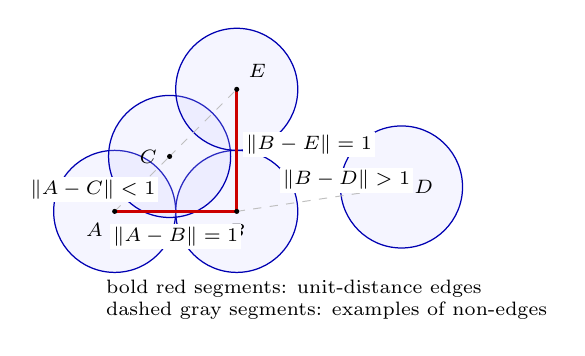
\begin{tikzpicture}[
  scale=1.55,
  halfdisk/.style={draw=blue!70!black, fill=blue!20, fill opacity=0.20, line width=0.45pt},
  unitedge/.style={draw=red!80!black, line width=1.0pt},
  pt/.style={circle, fill=black, inner sep=0.65pt},
  faint/.style={draw=gray!50, dashed, line width=0.35pt},
  lab/.style={font=\scriptsize, fill=white, inner sep=1pt}
]
  % points
  \coordinate (A) at (0,0);
  \coordinate (B) at (1,0);
  \coordinate (E) at (1,1);
  \coordinate (C) at (0.45,0.45);
  \coordinate (D) at (2.35,0.20);

  % half-unit disks
  \foreach \P in {A,B,C,D,E} {
    \draw[halfdisk] (\P) circle[radius=0.5];
  }

  % unit-distance edges in bold red
  \draw[unitedge] (A) -- (B);
  \draw[unitedge] (B) -- (E);

  % optional guide segments for one overlap and one separated pair
  \draw[faint] (A) -- (C);
  \draw[faint] (C) -- (E);
  \draw[faint] (B) -- (D);

  % points and labels
  \node[pt,label=below left:{\scriptsize $A$}] at (A) {};
  \node[pt,label=below:{\scriptsize $B$}] at (B) {};
  \node[pt,label=above right:{\scriptsize $E$}] at (E) {};
  \node[pt,label=left:{\scriptsize $C$}] at (C) {};
  \node[pt,label=right:{\scriptsize $D$}] at (D) {};

  % annotations
  \node[lab, anchor=north] at (0.5,-0.10) {$\|A-B\|=1$};
  \node[lab, anchor=west] at (1.05,0.55) {$\|B-E\|=1$};
  \node[lab, anchor=east] at (0.36,0.18) {$\|A-C\|<1$};
  \node[lab, anchor=south west] at (1.35,0.15) {$\|B-D\|>1$};

  % legend text
  \node[align=left, font=\scriptsize, anchor=west] at (-0.15,-0.72) {bold red segments: unit-distance edges\\dashed gray segments: examples of non-edges};
\end{tikzpicture}
\caption{A local point set showing the three relevant distance regimes simultaneously.  Bold red segments mark all pairs at distance $1$, hence all edges of the unit-distance graph on this five-point set.  The half-unit disks centered at $A$ and $C$ overlap because $\|A-C\|<1$, while the half-unit disks centered at $B$ and $D$ are separated because $\|B-D\|>1$.  Thus overlap between some half-unit disks is allowed; what matters combinatorially is only which pairs are exactly at distance $1$.}
\label{fig:touch-overlap-separate}
\end{figure}

\subsection{Hexagonal packing of half-unit disks}

The first example, shown in Figure~\ref{fig:hex-half-unit-packing}, is the standard hexagonal packing of disks of radius $1/2$, clipped so that all disks lie inside $[0,10]^2$; this is the classical optimal planar disk-packing pattern, going back to Fejes T\'oth \cite{FejesToth1942}.  The centers are
\[
  H=\left\{\left(\frac12+i+\frac{\varepsilon_j}{2},\frac12+\frac{\sqrt3}{2}j\right): j=0,\ldots,10\right\},
\]
where $\varepsilon_j=0$ for even rows and $\varepsilon_j=1$ for odd rows.  For even rows one takes $i=0,\ldots,9$, and for odd rows one takes $i=0,\ldots,8$.  Thus there are six rows with ten centers and five rows with nine centers, hence
\[
  |H|=6\cdot 10+5\cdot 9=105.
\]
Unit-distance edges occur horizontally and between adjacent shifted rows.  The horizontal count is
\[
  6\cdot 9+5\cdot 8=94,
\]
and each of the ten adjacent row pairs contributes $18$ diagonal contacts.  Hence
\[
  U(H)=94+10\cdot 18=274.
\]
Equivalently, the average degree of the resulting unit-distance graph is $2U(H)/|H|=548/105\approx5.219$.

\begin{figure}[p]
\centering
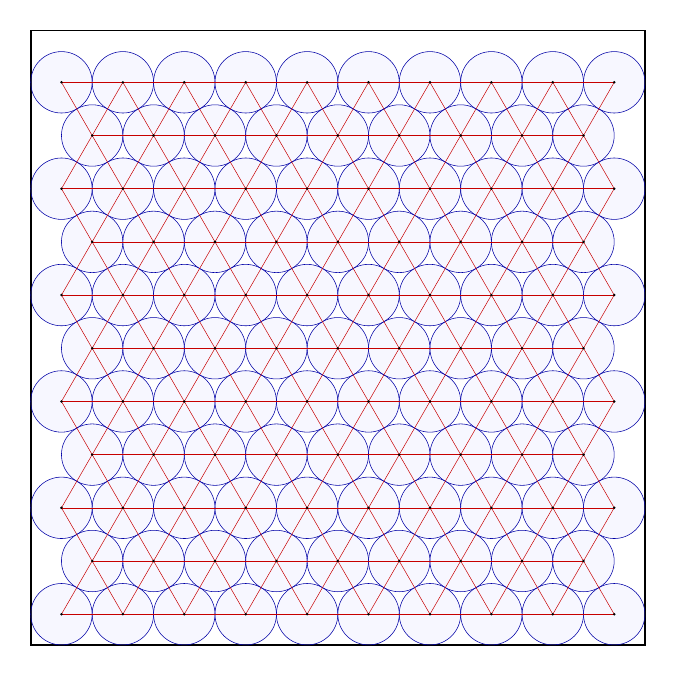
\begin{tikzpicture}[
  scale=0.78,
  halfdisk/.style={draw=blue!65!black, fill=blue!18, fill opacity=0.18, line width=0.20pt},
  unit/.style={draw=red!78!black, line width=0.18pt},
  pt/.style={circle, fill=black, inner sep=0.24pt},
  boundary/.style={draw=black, line width=0.55pt}
]
  \clip (-0.05,-0.05) rectangle (10.05,10.05);
  \draw[boundary] (0,0) rectangle (10,10);
  \draw[halfdisk] (0.5,0.5) circle[radius=0.5];
  \draw[halfdisk] (1.5,0.5) circle[radius=0.5];
  \draw[halfdisk] (2.5,0.5) circle[radius=0.5];
  \draw[halfdisk] (3.5,0.5) circle[radius=0.5];
  \draw[halfdisk] (4.5,0.5) circle[radius=0.5];
  \draw[halfdisk] (5.5,0.5) circle[radius=0.5];
  \draw[halfdisk] (6.5,0.5) circle[radius=0.5];
  \draw[halfdisk] (7.5,0.5) circle[radius=0.5];
  \draw[halfdisk] (8.5,0.5) circle[radius=0.5];
  \draw[halfdisk] (9.5,0.5) circle[radius=0.5];
  \draw[halfdisk] (1,1.366) circle[radius=0.5];
  \draw[halfdisk] (2,1.366) circle[radius=0.5];
  \draw[halfdisk] (3,1.366) circle[radius=0.5];
  \draw[halfdisk] (4,1.366) circle[radius=0.5];
  \draw[halfdisk] (5,1.366) circle[radius=0.5];
  \draw[halfdisk] (6,1.366) circle[radius=0.5];
  \draw[halfdisk] (7,1.366) circle[radius=0.5];
  \draw[halfdisk] (8,1.366) circle[radius=0.5];
  \draw[halfdisk] (9,1.366) circle[radius=0.5];
  \draw[halfdisk] (0.5,2.2321) circle[radius=0.5];
  \draw[halfdisk] (1.5,2.2321) circle[radius=0.5];
  \draw[halfdisk] (2.5,2.2321) circle[radius=0.5];
  \draw[halfdisk] (3.5,2.2321) circle[radius=0.5];
  \draw[halfdisk] (4.5,2.2321) circle[radius=0.5];
  \draw[halfdisk] (5.5,2.2321) circle[radius=0.5];
  \draw[halfdisk] (6.5,2.2321) circle[radius=0.5];
  \draw[halfdisk] (7.5,2.2321) circle[radius=0.5];
  \draw[halfdisk] (8.5,2.2321) circle[radius=0.5];
  \draw[halfdisk] (9.5,2.2321) circle[radius=0.5];
  \draw[halfdisk] (1,3.0981) circle[radius=0.5];
  \draw[halfdisk] (2,3.0981) circle[radius=0.5];
  \draw[halfdisk] (3,3.0981) circle[radius=0.5];
  \draw[halfdisk] (4,3.0981) circle[radius=0.5];
  \draw[halfdisk] (5,3.0981) circle[radius=0.5];
  \draw[halfdisk] (6,3.0981) circle[radius=0.5];
  \draw[halfdisk] (7,3.0981) circle[radius=0.5];
  \draw[halfdisk] (8,3.0981) circle[radius=0.5];
  \draw[halfdisk] (9,3.0981) circle[radius=0.5];
  \draw[halfdisk] (0.5,3.9641) circle[radius=0.5];
  \draw[halfdisk] (1.5,3.9641) circle[radius=0.5];
  \draw[halfdisk] (2.5,3.9641) circle[radius=0.5];
  \draw[halfdisk] (3.5,3.9641) circle[radius=0.5];
  \draw[halfdisk] (4.5,3.9641) circle[radius=0.5];
  \draw[halfdisk] (5.5,3.9641) circle[radius=0.5];
  \draw[halfdisk] (6.5,3.9641) circle[radius=0.5];
  \draw[halfdisk] (7.5,3.9641) circle[radius=0.5];
  \draw[halfdisk] (8.5,3.9641) circle[radius=0.5];
  \draw[halfdisk] (9.5,3.9641) circle[radius=0.5];
  \draw[halfdisk] (1,4.8301) circle[radius=0.5];
  \draw[halfdisk] (2,4.8301) circle[radius=0.5];
  \draw[halfdisk] (3,4.8301) circle[radius=0.5];
  \draw[halfdisk] (4,4.8301) circle[radius=0.5];
  \draw[halfdisk] (5,4.8301) circle[radius=0.5];
  \draw[halfdisk] (6,4.8301) circle[radius=0.5];
  \draw[halfdisk] (7,4.8301) circle[radius=0.5];
  \draw[halfdisk] (8,4.8301) circle[radius=0.5];
  \draw[halfdisk] (9,4.8301) circle[radius=0.5];
  \draw[halfdisk] (0.5,5.6962) circle[radius=0.5];
  \draw[halfdisk] (1.5,5.6962) circle[radius=0.5];
  \draw[halfdisk] (2.5,5.6962) circle[radius=0.5];
  \draw[halfdisk] (3.5,5.6962) circle[radius=0.5];
  \draw[halfdisk] (4.5,5.6962) circle[radius=0.5];
  \draw[halfdisk] (5.5,5.6962) circle[radius=0.5];
  \draw[halfdisk] (6.5,5.6962) circle[radius=0.5];
  \draw[halfdisk] (7.5,5.6962) circle[radius=0.5];
  \draw[halfdisk] (8.5,5.6962) circle[radius=0.5];
  \draw[halfdisk] (9.5,5.6962) circle[radius=0.5];
  \draw[halfdisk] (1,6.5622) circle[radius=0.5];
  \draw[halfdisk] (2,6.5622) circle[radius=0.5];
  \draw[halfdisk] (3,6.5622) circle[radius=0.5];
  \draw[halfdisk] (4,6.5622) circle[radius=0.5];
  \draw[halfdisk] (5,6.5622) circle[radius=0.5];
  \draw[halfdisk] (6,6.5622) circle[radius=0.5];
  \draw[halfdisk] (7,6.5622) circle[radius=0.5];
  \draw[halfdisk] (8,6.5622) circle[radius=0.5];
  \draw[halfdisk] (9,6.5622) circle[radius=0.5];
  \draw[halfdisk] (0.5,7.4282) circle[radius=0.5];
  \draw[halfdisk] (1.5,7.4282) circle[radius=0.5];
  \draw[halfdisk] (2.5,7.4282) circle[radius=0.5];
  \draw[halfdisk] (3.5,7.4282) circle[radius=0.5];
  \draw[halfdisk] (4.5,7.4282) circle[radius=0.5];
  \draw[halfdisk] (5.5,7.4282) circle[radius=0.5];
  \draw[halfdisk] (6.5,7.4282) circle[radius=0.5];
  \draw[halfdisk] (7.5,7.4282) circle[radius=0.5];
  \draw[halfdisk] (8.5,7.4282) circle[radius=0.5];
  \draw[halfdisk] (9.5,7.4282) circle[radius=0.5];
  \draw[halfdisk] (1,8.2942) circle[radius=0.5];
  \draw[halfdisk] (2,8.2942) circle[radius=0.5];
  \draw[halfdisk] (3,8.2942) circle[radius=0.5];
  \draw[halfdisk] (4,8.2942) circle[radius=0.5];
  \draw[halfdisk] (5,8.2942) circle[radius=0.5];
  \draw[halfdisk] (6,8.2942) circle[radius=0.5];
  \draw[halfdisk] (7,8.2942) circle[radius=0.5];
  \draw[halfdisk] (8,8.2942) circle[radius=0.5];
  \draw[halfdisk] (9,8.2942) circle[radius=0.5];
  \draw[halfdisk] (0.5,9.1603) circle[radius=0.5];
  \draw[halfdisk] (1.5,9.1603) circle[radius=0.5];
  \draw[halfdisk] (2.5,9.1603) circle[radius=0.5];
  \draw[halfdisk] (3.5,9.1603) circle[radius=0.5];
  \draw[halfdisk] (4.5,9.1603) circle[radius=0.5];
  \draw[halfdisk] (5.5,9.1603) circle[radius=0.5];
  \draw[halfdisk] (6.5,9.1603) circle[radius=0.5];
  \draw[halfdisk] (7.5,9.1603) circle[radius=0.5];
  \draw[halfdisk] (8.5,9.1603) circle[radius=0.5];
  \draw[halfdisk] (9.5,9.1603) circle[radius=0.5];
  \draw[unit] (0.5,0.5) -- (1.5,0.5);
  \draw[unit] (0.5,0.5) -- (1,1.366);
  \draw[unit] (1.5,0.5) -- (2.5,0.5);
  \draw[unit] (1.5,0.5) -- (1,1.366);
  \draw[unit] (1.5,0.5) -- (2,1.366);
  \draw[unit] (2.5,0.5) -- (3.5,0.5);
  \draw[unit] (2.5,0.5) -- (2,1.366);
  \draw[unit] (2.5,0.5) -- (3,1.366);
  \draw[unit] (3.5,0.5) -- (4.5,0.5);
  \draw[unit] (3.5,0.5) -- (3,1.366);
  \draw[unit] (3.5,0.5) -- (4,1.366);
  \draw[unit] (4.5,0.5) -- (5.5,0.5);
  \draw[unit] (4.5,0.5) -- (4,1.366);
  \draw[unit] (4.5,0.5) -- (5,1.366);
  \draw[unit] (5.5,0.5) -- (6.5,0.5);
  \draw[unit] (5.5,0.5) -- (5,1.366);
  \draw[unit] (5.5,0.5) -- (6,1.366);
  \draw[unit] (6.5,0.5) -- (7.5,0.5);
  \draw[unit] (6.5,0.5) -- (6,1.366);
  \draw[unit] (6.5,0.5) -- (7,1.366);
  \draw[unit] (7.5,0.5) -- (8.5,0.5);
  \draw[unit] (7.5,0.5) -- (7,1.366);
  \draw[unit] (7.5,0.5) -- (8,1.366);
  \draw[unit] (8.5,0.5) -- (9.5,0.5);
  \draw[unit] (8.5,0.5) -- (8,1.366);
  \draw[unit] (8.5,0.5) -- (9,1.366);
  \draw[unit] (9.5,0.5) -- (9,1.366);
  \draw[unit] (1,1.366) -- (2,1.366);
  \draw[unit] (1,1.366) -- (0.5,2.2321);
  \draw[unit] (1,1.366) -- (1.5,2.2321);
  \draw[unit] (2,1.366) -- (3,1.366);
  \draw[unit] (2,1.366) -- (1.5,2.2321);
  \draw[unit] (2,1.366) -- (2.5,2.2321);
  \draw[unit] (3,1.366) -- (4,1.366);
  \draw[unit] (3,1.366) -- (2.5,2.2321);
  \draw[unit] (3,1.366) -- (3.5,2.2321);
  \draw[unit] (4,1.366) -- (5,1.366);
  \draw[unit] (4,1.366) -- (3.5,2.2321);
  \draw[unit] (4,1.366) -- (4.5,2.2321);
  \draw[unit] (5,1.366) -- (6,1.366);
  \draw[unit] (5,1.366) -- (4.5,2.2321);
  \draw[unit] (5,1.366) -- (5.5,2.2321);
  \draw[unit] (6,1.366) -- (7,1.366);
  \draw[unit] (6,1.366) -- (5.5,2.2321);
  \draw[unit] (6,1.366) -- (6.5,2.2321);
  \draw[unit] (7,1.366) -- (8,1.366);
  \draw[unit] (7,1.366) -- (6.5,2.2321);
  \draw[unit] (7,1.366) -- (7.5,2.2321);
  \draw[unit] (8,1.366) -- (9,1.366);
  \draw[unit] (8,1.366) -- (7.5,2.2321);
  \draw[unit] (8,1.366) -- (8.5,2.2321);
  \draw[unit] (9,1.366) -- (8.5,2.2321);
  \draw[unit] (9,1.366) -- (9.5,2.2321);
  \draw[unit] (0.5,2.2321) -- (1.5,2.2321);
  \draw[unit] (0.5,2.2321) -- (1,3.0981);
  \draw[unit] (1.5,2.2321) -- (2.5,2.2321);
  \draw[unit] (1.5,2.2321) -- (1,3.0981);
  \draw[unit] (1.5,2.2321) -- (2,3.0981);
  \draw[unit] (2.5,2.2321) -- (3.5,2.2321);
  \draw[unit] (2.5,2.2321) -- (2,3.0981);
  \draw[unit] (2.5,2.2321) -- (3,3.0981);
  \draw[unit] (3.5,2.2321) -- (4.5,2.2321);
  \draw[unit] (3.5,2.2321) -- (3,3.0981);
  \draw[unit] (3.5,2.2321) -- (4,3.0981);
  \draw[unit] (4.5,2.2321) -- (5.5,2.2321);
  \draw[unit] (4.5,2.2321) -- (4,3.0981);
  \draw[unit] (4.5,2.2321) -- (5,3.0981);
  \draw[unit] (5.5,2.2321) -- (6.5,2.2321);
  \draw[unit] (5.5,2.2321) -- (5,3.0981);
  \draw[unit] (5.5,2.2321) -- (6,3.0981);
  \draw[unit] (6.5,2.2321) -- (7.5,2.2321);
  \draw[unit] (6.5,2.2321) -- (6,3.0981);
  \draw[unit] (6.5,2.2321) -- (7,3.0981);
  \draw[unit] (7.5,2.2321) -- (8.5,2.2321);
  \draw[unit] (7.5,2.2321) -- (7,3.0981);
  \draw[unit] (7.5,2.2321) -- (8,3.0981);
  \draw[unit] (8.5,2.2321) -- (9.5,2.2321);
  \draw[unit] (8.5,2.2321) -- (8,3.0981);
  \draw[unit] (8.5,2.2321) -- (9,3.0981);
  \draw[unit] (9.5,2.2321) -- (9,3.0981);
  \draw[unit] (1,3.0981) -- (2,3.0981);
  \draw[unit] (1,3.0981) -- (0.5,3.9641);
  \draw[unit] (1,3.0981) -- (1.5,3.9641);
  \draw[unit] (2,3.0981) -- (3,3.0981);
  \draw[unit] (2,3.0981) -- (1.5,3.9641);
  \draw[unit] (2,3.0981) -- (2.5,3.9641);
  \draw[unit] (3,3.0981) -- (4,3.0981);
  \draw[unit] (3,3.0981) -- (2.5,3.9641);
  \draw[unit] (3,3.0981) -- (3.5,3.9641);
  \draw[unit] (4,3.0981) -- (5,3.0981);
  \draw[unit] (4,3.0981) -- (3.5,3.9641);
  \draw[unit] (4,3.0981) -- (4.5,3.9641);
  \draw[unit] (5,3.0981) -- (6,3.0981);
  \draw[unit] (5,3.0981) -- (4.5,3.9641);
  \draw[unit] (5,3.0981) -- (5.5,3.9641);
  \draw[unit] (6,3.0981) -- (7,3.0981);
  \draw[unit] (6,3.0981) -- (5.5,3.9641);
  \draw[unit] (6,3.0981) -- (6.5,3.9641);
  \draw[unit] (7,3.0981) -- (8,3.0981);
  \draw[unit] (7,3.0981) -- (6.5,3.9641);
  \draw[unit] (7,3.0981) -- (7.5,3.9641);
  \draw[unit] (8,3.0981) -- (9,3.0981);
  \draw[unit] (8,3.0981) -- (7.5,3.9641);
  \draw[unit] (8,3.0981) -- (8.5,3.9641);
  \draw[unit] (9,3.0981) -- (8.5,3.9641);
  \draw[unit] (9,3.0981) -- (9.5,3.9641);
  \draw[unit] (0.5,3.9641) -- (1.5,3.9641);
  \draw[unit] (0.5,3.9641) -- (1,4.8301);
  \draw[unit] (1.5,3.9641) -- (2.5,3.9641);
  \draw[unit] (1.5,3.9641) -- (1,4.8301);
  \draw[unit] (1.5,3.9641) -- (2,4.8301);
  \draw[unit] (2.5,3.9641) -- (3.5,3.9641);
  \draw[unit] (2.5,3.9641) -- (2,4.8301);
  \draw[unit] (2.5,3.9641) -- (3,4.8301);
  \draw[unit] (3.5,3.9641) -- (4.5,3.9641);
  \draw[unit] (3.5,3.9641) -- (3,4.8301);
  \draw[unit] (3.5,3.9641) -- (4,4.8301);
  \draw[unit] (4.5,3.9641) -- (5.5,3.9641);
  \draw[unit] (4.5,3.9641) -- (4,4.8301);
  \draw[unit] (4.5,3.9641) -- (5,4.8301);
  \draw[unit] (5.5,3.9641) -- (6.5,3.9641);
  \draw[unit] (5.5,3.9641) -- (5,4.8301);
  \draw[unit] (5.5,3.9641) -- (6,4.8301);
  \draw[unit] (6.5,3.9641) -- (7.5,3.9641);
  \draw[unit] (6.5,3.9641) -- (6,4.8301);
  \draw[unit] (6.5,3.9641) -- (7,4.8301);
  \draw[unit] (7.5,3.9641) -- (8.5,3.9641);
  \draw[unit] (7.5,3.9641) -- (7,4.8301);
  \draw[unit] (7.5,3.9641) -- (8,4.8301);
  \draw[unit] (8.5,3.9641) -- (9.5,3.9641);
  \draw[unit] (8.5,3.9641) -- (8,4.8301);
  \draw[unit] (8.5,3.9641) -- (9,4.8301);
  \draw[unit] (9.5,3.9641) -- (9,4.8301);
  \draw[unit] (1,4.8301) -- (2,4.8301);
  \draw[unit] (1,4.8301) -- (0.5,5.6962);
  \draw[unit] (1,4.8301) -- (1.5,5.6962);
  \draw[unit] (2,4.8301) -- (3,4.8301);
  \draw[unit] (2,4.8301) -- (1.5,5.6962);
  \draw[unit] (2,4.8301) -- (2.5,5.6962);
  \draw[unit] (3,4.8301) -- (4,4.8301);
  \draw[unit] (3,4.8301) -- (2.5,5.6962);
  \draw[unit] (3,4.8301) -- (3.5,5.6962);
  \draw[unit] (4,4.8301) -- (5,4.8301);
  \draw[unit] (4,4.8301) -- (3.5,5.6962);
  \draw[unit] (4,4.8301) -- (4.5,5.6962);
  \draw[unit] (5,4.8301) -- (6,4.8301);
  \draw[unit] (5,4.8301) -- (4.5,5.6962);
  \draw[unit] (5,4.8301) -- (5.5,5.6962);
  \draw[unit] (6,4.8301) -- (7,4.8301);
  \draw[unit] (6,4.8301) -- (5.5,5.6962);
  \draw[unit] (6,4.8301) -- (6.5,5.6962);
  \draw[unit] (7,4.8301) -- (8,4.8301);
  \draw[unit] (7,4.8301) -- (6.5,5.6962);
  \draw[unit] (7,4.8301) -- (7.5,5.6962);
  \draw[unit] (8,4.8301) -- (9,4.8301);
  \draw[unit] (8,4.8301) -- (7.5,5.6962);
  \draw[unit] (8,4.8301) -- (8.5,5.6962);
  \draw[unit] (9,4.8301) -- (8.5,5.6962);
  \draw[unit] (9,4.8301) -- (9.5,5.6962);
  \draw[unit] (0.5,5.6962) -- (1.5,5.6962);
  \draw[unit] (0.5,5.6962) -- (1,6.5622);
  \draw[unit] (1.5,5.6962) -- (2.5,5.6962);
  \draw[unit] (1.5,5.6962) -- (1,6.5622);
  \draw[unit] (1.5,5.6962) -- (2,6.5622);
  \draw[unit] (2.5,5.6962) -- (3.5,5.6962);
  \draw[unit] (2.5,5.6962) -- (2,6.5622);
  \draw[unit] (2.5,5.6962) -- (3,6.5622);
  \draw[unit] (3.5,5.6962) -- (4.5,5.6962);
  \draw[unit] (3.5,5.6962) -- (3,6.5622);
  \draw[unit] (3.5,5.6962) -- (4,6.5622);
  \draw[unit] (4.5,5.6962) -- (5.5,5.6962);
  \draw[unit] (4.5,5.6962) -- (4,6.5622);
  \draw[unit] (4.5,5.6962) -- (5,6.5622);
  \draw[unit] (5.5,5.6962) -- (6.5,5.6962);
  \draw[unit] (5.5,5.6962) -- (5,6.5622);
  \draw[unit] (5.5,5.6962) -- (6,6.5622);
  \draw[unit] (6.5,5.6962) -- (7.5,5.6962);
  \draw[unit] (6.5,5.6962) -- (6,6.5622);
  \draw[unit] (6.5,5.6962) -- (7,6.5622);
  \draw[unit] (7.5,5.6962) -- (8.5,5.6962);
  \draw[unit] (7.5,5.6962) -- (7,6.5622);
  \draw[unit] (7.5,5.6962) -- (8,6.5622);
  \draw[unit] (8.5,5.6962) -- (9.5,5.6962);
  \draw[unit] (8.5,5.6962) -- (8,6.5622);
  \draw[unit] (8.5,5.6962) -- (9,6.5622);
  \draw[unit] (9.5,5.6962) -- (9,6.5622);
  \draw[unit] (1,6.5622) -- (2,6.5622);
  \draw[unit] (1,6.5622) -- (0.5,7.4282);
  \draw[unit] (1,6.5622) -- (1.5,7.4282);
  \draw[unit] (2,6.5622) -- (3,6.5622);
  \draw[unit] (2,6.5622) -- (1.5,7.4282);
  \draw[unit] (2,6.5622) -- (2.5,7.4282);
  \draw[unit] (3,6.5622) -- (4,6.5622);
  \draw[unit] (3,6.5622) -- (2.5,7.4282);
  \draw[unit] (3,6.5622) -- (3.5,7.4282);
  \draw[unit] (4,6.5622) -- (5,6.5622);
  \draw[unit] (4,6.5622) -- (3.5,7.4282);
  \draw[unit] (4,6.5622) -- (4.5,7.4282);
  \draw[unit] (5,6.5622) -- (6,6.5622);
  \draw[unit] (5,6.5622) -- (4.5,7.4282);
  \draw[unit] (5,6.5622) -- (5.5,7.4282);
  \draw[unit] (6,6.5622) -- (7,6.5622);
  \draw[unit] (6,6.5622) -- (5.5,7.4282);
  \draw[unit] (6,6.5622) -- (6.5,7.4282);
  \draw[unit] (7,6.5622) -- (8,6.5622);
  \draw[unit] (7,6.5622) -- (6.5,7.4282);
  \draw[unit] (7,6.5622) -- (7.5,7.4282);
  \draw[unit] (8,6.5622) -- (9,6.5622);
  \draw[unit] (8,6.5622) -- (7.5,7.4282);
  \draw[unit] (8,6.5622) -- (8.5,7.4282);
  \draw[unit] (9,6.5622) -- (8.5,7.4282);
  \draw[unit] (9,6.5622) -- (9.5,7.4282);
  \draw[unit] (0.5,7.4282) -- (1.5,7.4282);
  \draw[unit] (0.5,7.4282) -- (1,8.2942);
  \draw[unit] (1.5,7.4282) -- (2.5,7.4282);
  \draw[unit] (1.5,7.4282) -- (1,8.2942);
  \draw[unit] (1.5,7.4282) -- (2,8.2942);
  \draw[unit] (2.5,7.4282) -- (3.5,7.4282);
  \draw[unit] (2.5,7.4282) -- (2,8.2942);
  \draw[unit] (2.5,7.4282) -- (3,8.2942);
  \draw[unit] (3.5,7.4282) -- (4.5,7.4282);
  \draw[unit] (3.5,7.4282) -- (3,8.2942);
  \draw[unit] (3.5,7.4282) -- (4,8.2942);
  \draw[unit] (4.5,7.4282) -- (5.5,7.4282);
  \draw[unit] (4.5,7.4282) -- (4,8.2942);
  \draw[unit] (4.5,7.4282) -- (5,8.2942);
  \draw[unit] (5.5,7.4282) -- (6.5,7.4282);
  \draw[unit] (5.5,7.4282) -- (5,8.2942);
  \draw[unit] (5.5,7.4282) -- (6,8.2942);
  \draw[unit] (6.5,7.4282) -- (7.5,7.4282);
  \draw[unit] (6.5,7.4282) -- (6,8.2942);
  \draw[unit] (6.5,7.4282) -- (7,8.2942);
  \draw[unit] (7.5,7.4282) -- (8.5,7.4282);
  \draw[unit] (7.5,7.4282) -- (7,8.2942);
  \draw[unit] (7.5,7.4282) -- (8,8.2942);
  \draw[unit] (8.5,7.4282) -- (9.5,7.4282);
  \draw[unit] (8.5,7.4282) -- (8,8.2942);
  \draw[unit] (8.5,7.4282) -- (9,8.2942);
  \draw[unit] (9.5,7.4282) -- (9,8.2942);
  \draw[unit] (1,8.2942) -- (2,8.2942);
  \draw[unit] (1,8.2942) -- (0.5,9.1603);
  \draw[unit] (1,8.2942) -- (1.5,9.1603);
  \draw[unit] (2,8.2942) -- (3,8.2942);
  \draw[unit] (2,8.2942) -- (1.5,9.1603);
  \draw[unit] (2,8.2942) -- (2.5,9.1603);
  \draw[unit] (3,8.2942) -- (4,8.2942);
  \draw[unit] (3,8.2942) -- (2.5,9.1603);
  \draw[unit] (3,8.2942) -- (3.5,9.1603);
  \draw[unit] (4,8.2942) -- (5,8.2942);
  \draw[unit] (4,8.2942) -- (3.5,9.1603);
  \draw[unit] (4,8.2942) -- (4.5,9.1603);
  \draw[unit] (5,8.2942) -- (6,8.2942);
  \draw[unit] (5,8.2942) -- (4.5,9.1603);
  \draw[unit] (5,8.2942) -- (5.5,9.1603);
  \draw[unit] (6,8.2942) -- (7,8.2942);
  \draw[unit] (6,8.2942) -- (5.5,9.1603);
  \draw[unit] (6,8.2942) -- (6.5,9.1603);
  \draw[unit] (7,8.2942) -- (8,8.2942);
  \draw[unit] (7,8.2942) -- (6.5,9.1603);
  \draw[unit] (7,8.2942) -- (7.5,9.1603);
  \draw[unit] (8,8.2942) -- (9,8.2942);
  \draw[unit] (8,8.2942) -- (7.5,9.1603);
  \draw[unit] (8,8.2942) -- (8.5,9.1603);
  \draw[unit] (9,8.2942) -- (8.5,9.1603);
  \draw[unit] (9,8.2942) -- (9.5,9.1603);
  \draw[unit] (0.5,9.1603) -- (1.5,9.1603);
  \draw[unit] (1.5,9.1603) -- (2.5,9.1603);
  \draw[unit] (2.5,9.1603) -- (3.5,9.1603);
  \draw[unit] (3.5,9.1603) -- (4.5,9.1603);
  \draw[unit] (4.5,9.1603) -- (5.5,9.1603);
  \draw[unit] (5.5,9.1603) -- (6.5,9.1603);
  \draw[unit] (6.5,9.1603) -- (7.5,9.1603);
  \draw[unit] (7.5,9.1603) -- (8.5,9.1603);
  \draw[unit] (8.5,9.1603) -- (9.5,9.1603);
  \node[pt] at (0.5,0.5) {};
  \node[pt] at (1.5,0.5) {};
  \node[pt] at (2.5,0.5) {};
  \node[pt] at (3.5,0.5) {};
  \node[pt] at (4.5,0.5) {};
  \node[pt] at (5.5,0.5) {};
  \node[pt] at (6.5,0.5) {};
  \node[pt] at (7.5,0.5) {};
  \node[pt] at (8.5,0.5) {};
  \node[pt] at (9.5,0.5) {};
  \node[pt] at (1,1.366) {};
  \node[pt] at (2,1.366) {};
  \node[pt] at (3,1.366) {};
  \node[pt] at (4,1.366) {};
  \node[pt] at (5,1.366) {};
  \node[pt] at (6,1.366) {};
  \node[pt] at (7,1.366) {};
  \node[pt] at (8,1.366) {};
  \node[pt] at (9,1.366) {};
  \node[pt] at (0.5,2.2321) {};
  \node[pt] at (1.5,2.2321) {};
  \node[pt] at (2.5,2.2321) {};
  \node[pt] at (3.5,2.2321) {};
  \node[pt] at (4.5,2.2321) {};
  \node[pt] at (5.5,2.2321) {};
  \node[pt] at (6.5,2.2321) {};
  \node[pt] at (7.5,2.2321) {};
  \node[pt] at (8.5,2.2321) {};
  \node[pt] at (9.5,2.2321) {};
  \node[pt] at (1,3.0981) {};
  \node[pt] at (2,3.0981) {};
  \node[pt] at (3,3.0981) {};
  \node[pt] at (4,3.0981) {};
  \node[pt] at (5,3.0981) {};
  \node[pt] at (6,3.0981) {};
  \node[pt] at (7,3.0981) {};
  \node[pt] at (8,3.0981) {};
  \node[pt] at (9,3.0981) {};
  \node[pt] at (0.5,3.9641) {};
  \node[pt] at (1.5,3.9641) {};
  \node[pt] at (2.5,3.9641) {};
  \node[pt] at (3.5,3.9641) {};
  \node[pt] at (4.5,3.9641) {};
  \node[pt] at (5.5,3.9641) {};
  \node[pt] at (6.5,3.9641) {};
  \node[pt] at (7.5,3.9641) {};
  \node[pt] at (8.5,3.9641) {};
  \node[pt] at (9.5,3.9641) {};
  \node[pt] at (1,4.8301) {};
  \node[pt] at (2,4.8301) {};
  \node[pt] at (3,4.8301) {};
  \node[pt] at (4,4.8301) {};
  \node[pt] at (5,4.8301) {};
  \node[pt] at (6,4.8301) {};
  \node[pt] at (7,4.8301) {};
  \node[pt] at (8,4.8301) {};
  \node[pt] at (9,4.8301) {};
  \node[pt] at (0.5,5.6962) {};
  \node[pt] at (1.5,5.6962) {};
  \node[pt] at (2.5,5.6962) {};
  \node[pt] at (3.5,5.6962) {};
  \node[pt] at (4.5,5.6962) {};
  \node[pt] at (5.5,5.6962) {};
  \node[pt] at (6.5,5.6962) {};
  \node[pt] at (7.5,5.6962) {};
  \node[pt] at (8.5,5.6962) {};
  \node[pt] at (9.5,5.6962) {};
  \node[pt] at (1,6.5622) {};
  \node[pt] at (2,6.5622) {};
  \node[pt] at (3,6.5622) {};
  \node[pt] at (4,6.5622) {};
  \node[pt] at (5,6.5622) {};
  \node[pt] at (6,6.5622) {};
  \node[pt] at (7,6.5622) {};
  \node[pt] at (8,6.5622) {};
  \node[pt] at (9,6.5622) {};
  \node[pt] at (0.5,7.4282) {};
  \node[pt] at (1.5,7.4282) {};
  \node[pt] at (2.5,7.4282) {};
  \node[pt] at (3.5,7.4282) {};
  \node[pt] at (4.5,7.4282) {};
  \node[pt] at (5.5,7.4282) {};
  \node[pt] at (6.5,7.4282) {};
  \node[pt] at (7.5,7.4282) {};
  \node[pt] at (8.5,7.4282) {};
  \node[pt] at (9.5,7.4282) {};
  \node[pt] at (1,8.2942) {};
  \node[pt] at (2,8.2942) {};
  \node[pt] at (3,8.2942) {};
  \node[pt] at (4,8.2942) {};
  \node[pt] at (5,8.2942) {};
  \node[pt] at (6,8.2942) {};
  \node[pt] at (7,8.2942) {};
  \node[pt] at (8,8.2942) {};
  \node[pt] at (9,8.2942) {};
  \node[pt] at (0.5,9.1603) {};
  \node[pt] at (1.5,9.1603) {};
  \node[pt] at (2.5,9.1603) {};
  \node[pt] at (3.5,9.1603) {};
  \node[pt] at (4.5,9.1603) {};
  \node[pt] at (5.5,9.1603) {};
  \node[pt] at (6.5,9.1603) {};
  \node[pt] at (7.5,9.1603) {};
  \node[pt] at (8.5,9.1603) {};
  \node[pt] at (9.5,9.1603) {};
\end{tikzpicture}
\caption{Hexagonal packing of half-unit disks in $[0,10]^2$.  There are $105$ centers and $274$ unit-distance pairs.  The disks have radius $1/2$ and are non-overlapping; red segments mark exactly the center pairs at distance $1$.}
\label{fig:hex-half-unit-packing}
\end{figure}

\subsection{A multidirectional integer lattice in the same square}\label{subsec:explicit-comparator}

The second example uses the integer grid before rescaling, but takes unit distances from several equal-length integer displacement vectors.  Let
\[
  L=\left\{\left(\frac{i}{\sqrt5},\frac{j}{\sqrt5}\right): i,j=0,1,\ldots,22\right\}\subset[0,10]^2.
\]
The upper index $22$ is chosen because $22/\sqrt5<10$, while $23/\sqrt5>10$.  Thus
\[
  |L|=23^2=529.
\]
The four undirected displacement types
\[
  (1,2),\quad (1,-2),\quad (2,1),\quad (2,-1)
\]
have squared length $5$ in the integer grid and therefore become unit displacement vectors after division by $\sqrt5$.  For each type, the number of valid translated copies inside the $23\times23$ integer grid is
\[
  (23-1)(23-2)=22\cdot21.
\]
Consequently
\[
  U(L)=4\cdot22\cdot21=1848.
\]
The average degree is $2U(L)/|L|=3696/529\approx6.988$, which is larger than for the hexagonal packing above.  This comparison is possible because the unit-distance problem is not a packing problem: in Figure~\ref{fig:multidirectional-lattice-0-10}, the half-unit disks are visual distance markers and may overlap, but edges are drawn only between centers exactly one unit apart.

To make the local structure easier to read, Figure~\ref{fig:multidirectional-lattice-local} also shows a small patch of the same multidirectional lattice in the window $[-2,2]^2$.  This local view makes the repeated pattern generated by the four displacement types $(\pm1,\pm2)$ and $(\pm2,\pm1)$ more apparent, while using exactly the same point set and edge rule as the larger plot.

\begin{figure}[p]
\centering
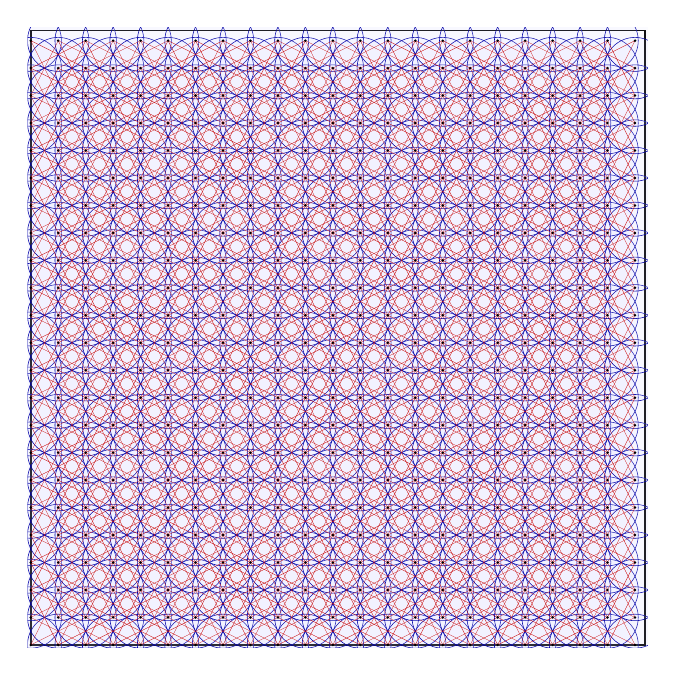
\begin{tikzpicture}[
  scale=0.78,
  halfdisk/.style={draw=blue!65!black, fill=blue!18, fill opacity=0.08, line width=0.20pt},
  unit/.style={draw=red!78!black, line width=0.10pt},
  pt/.style={circle, fill=black, inner sep=0.16pt},
  boundary/.style={draw=black, line width=0.55pt}
]
  \clip (-0.05,-0.05) rectangle (10.05,10.05);
  \draw[boundary] (0,0) rectangle (10,10);
  \draw[halfdisk] (0,0) circle[radius=0.5];
  \draw[halfdisk] (0,0.4472) circle[radius=0.5];
  \draw[halfdisk] (0,0.8944) circle[radius=0.5];
  \draw[halfdisk] (0,1.3416) circle[radius=0.5];
  \draw[halfdisk] (0,1.7889) circle[radius=0.5];
  \draw[halfdisk] (0,2.2361) circle[radius=0.5];
  \draw[halfdisk] (0,2.6833) circle[radius=0.5];
  \draw[halfdisk] (0,3.1305) circle[radius=0.5];
  \draw[halfdisk] (0,3.5777) circle[radius=0.5];
  \draw[halfdisk] (0,4.0249) circle[radius=0.5];
  \draw[halfdisk] (0,4.4721) circle[radius=0.5];
  \draw[halfdisk] (0,4.9193) circle[radius=0.5];
  \draw[halfdisk] (0,5.3666) circle[radius=0.5];
  \draw[halfdisk] (0,5.8138) circle[radius=0.5];
  \draw[halfdisk] (0,6.261) circle[radius=0.5];
  \draw[halfdisk] (0,6.7082) circle[radius=0.5];
  \draw[halfdisk] (0,7.1554) circle[radius=0.5];
  \draw[halfdisk] (0,7.6026) circle[radius=0.5];
  \draw[halfdisk] (0,8.0498) circle[radius=0.5];
  \draw[halfdisk] (0,8.4971) circle[radius=0.5];
  \draw[halfdisk] (0,8.9443) circle[radius=0.5];
  \draw[halfdisk] (0,9.3915) circle[radius=0.5];
  \draw[halfdisk] (0,9.8387) circle[radius=0.5];
  \draw[halfdisk] (0.4472,0) circle[radius=0.5];
  \draw[halfdisk] (0.4472,0.4472) circle[radius=0.5];
  \draw[halfdisk] (0.4472,0.8944) circle[radius=0.5];
  \draw[halfdisk] (0.4472,1.3416) circle[radius=0.5];
  \draw[halfdisk] (0.4472,1.7889) circle[radius=0.5];
  \draw[halfdisk] (0.4472,2.2361) circle[radius=0.5];
  \draw[halfdisk] (0.4472,2.6833) circle[radius=0.5];
  \draw[halfdisk] (0.4472,3.1305) circle[radius=0.5];
  \draw[halfdisk] (0.4472,3.5777) circle[radius=0.5];
  \draw[halfdisk] (0.4472,4.0249) circle[radius=0.5];
  \draw[halfdisk] (0.4472,4.4721) circle[radius=0.5];
  \draw[halfdisk] (0.4472,4.9193) circle[radius=0.5];
  \draw[halfdisk] (0.4472,5.3666) circle[radius=0.5];
  \draw[halfdisk] (0.4472,5.8138) circle[radius=0.5];
  \draw[halfdisk] (0.4472,6.261) circle[radius=0.5];
  \draw[halfdisk] (0.4472,6.7082) circle[radius=0.5];
  \draw[halfdisk] (0.4472,7.1554) circle[radius=0.5];
  \draw[halfdisk] (0.4472,7.6026) circle[radius=0.5];
  \draw[halfdisk] (0.4472,8.0498) circle[radius=0.5];
  \draw[halfdisk] (0.4472,8.4971) circle[radius=0.5];
  \draw[halfdisk] (0.4472,8.9443) circle[radius=0.5];
  \draw[halfdisk] (0.4472,9.3915) circle[radius=0.5];
  \draw[halfdisk] (0.4472,9.8387) circle[radius=0.5];
  \draw[halfdisk] (0.8944,0) circle[radius=0.5];
  \draw[halfdisk] (0.8944,0.4472) circle[radius=0.5];
  \draw[halfdisk] (0.8944,0.8944) circle[radius=0.5];
  \draw[halfdisk] (0.8944,1.3416) circle[radius=0.5];
  \draw[halfdisk] (0.8944,1.7889) circle[radius=0.5];
  \draw[halfdisk] (0.8944,2.2361) circle[radius=0.5];
  \draw[halfdisk] (0.8944,2.6833) circle[radius=0.5];
  \draw[halfdisk] (0.8944,3.1305) circle[radius=0.5];
  \draw[halfdisk] (0.8944,3.5777) circle[radius=0.5];
  \draw[halfdisk] (0.8944,4.0249) circle[radius=0.5];
  \draw[halfdisk] (0.8944,4.4721) circle[radius=0.5];
  \draw[halfdisk] (0.8944,4.9193) circle[radius=0.5];
  \draw[halfdisk] (0.8944,5.3666) circle[radius=0.5];
  \draw[halfdisk] (0.8944,5.8138) circle[radius=0.5];
  \draw[halfdisk] (0.8944,6.261) circle[radius=0.5];
  \draw[halfdisk] (0.8944,6.7082) circle[radius=0.5];
  \draw[halfdisk] (0.8944,7.1554) circle[radius=0.5];
  \draw[halfdisk] (0.8944,7.6026) circle[radius=0.5];
  \draw[halfdisk] (0.8944,8.0498) circle[radius=0.5];
  \draw[halfdisk] (0.8944,8.4971) circle[radius=0.5];
  \draw[halfdisk] (0.8944,8.9443) circle[radius=0.5];
  \draw[halfdisk] (0.8944,9.3915) circle[radius=0.5];
  \draw[halfdisk] (0.8944,9.8387) circle[radius=0.5];
  \draw[halfdisk] (1.3416,0) circle[radius=0.5];
  \draw[halfdisk] (1.3416,0.4472) circle[radius=0.5];
  \draw[halfdisk] (1.3416,0.8944) circle[radius=0.5];
  \draw[halfdisk] (1.3416,1.3416) circle[radius=0.5];
  \draw[halfdisk] (1.3416,1.7889) circle[radius=0.5];
  \draw[halfdisk] (1.3416,2.2361) circle[radius=0.5];
  \draw[halfdisk] (1.3416,2.6833) circle[radius=0.5];
  \draw[halfdisk] (1.3416,3.1305) circle[radius=0.5];
  \draw[halfdisk] (1.3416,3.5777) circle[radius=0.5];
  \draw[halfdisk] (1.3416,4.0249) circle[radius=0.5];
  \draw[halfdisk] (1.3416,4.4721) circle[radius=0.5];
  \draw[halfdisk] (1.3416,4.9193) circle[radius=0.5];
  \draw[halfdisk] (1.3416,5.3666) circle[radius=0.5];
  \draw[halfdisk] (1.3416,5.8138) circle[radius=0.5];
  \draw[halfdisk] (1.3416,6.261) circle[radius=0.5];
  \draw[halfdisk] (1.3416,6.7082) circle[radius=0.5];
  \draw[halfdisk] (1.3416,7.1554) circle[radius=0.5];
  \draw[halfdisk] (1.3416,7.6026) circle[radius=0.5];
  \draw[halfdisk] (1.3416,8.0498) circle[radius=0.5];
  \draw[halfdisk] (1.3416,8.4971) circle[radius=0.5];
  \draw[halfdisk] (1.3416,8.9443) circle[radius=0.5];
  \draw[halfdisk] (1.3416,9.3915) circle[radius=0.5];
  \draw[halfdisk] (1.3416,9.8387) circle[radius=0.5];
  \draw[halfdisk] (1.7889,0) circle[radius=0.5];
  \draw[halfdisk] (1.7889,0.4472) circle[radius=0.5];
  \draw[halfdisk] (1.7889,0.8944) circle[radius=0.5];
  \draw[halfdisk] (1.7889,1.3416) circle[radius=0.5];
  \draw[halfdisk] (1.7889,1.7889) circle[radius=0.5];
  \draw[halfdisk] (1.7889,2.2361) circle[radius=0.5];
  \draw[halfdisk] (1.7889,2.6833) circle[radius=0.5];
  \draw[halfdisk] (1.7889,3.1305) circle[radius=0.5];
  \draw[halfdisk] (1.7889,3.5777) circle[radius=0.5];
  \draw[halfdisk] (1.7889,4.0249) circle[radius=0.5];
  \draw[halfdisk] (1.7889,4.4721) circle[radius=0.5];
  \draw[halfdisk] (1.7889,4.9193) circle[radius=0.5];
  \draw[halfdisk] (1.7889,5.3666) circle[radius=0.5];
  \draw[halfdisk] (1.7889,5.8138) circle[radius=0.5];
  \draw[halfdisk] (1.7889,6.261) circle[radius=0.5];
  \draw[halfdisk] (1.7889,6.7082) circle[radius=0.5];
  \draw[halfdisk] (1.7889,7.1554) circle[radius=0.5];
  \draw[halfdisk] (1.7889,7.6026) circle[radius=0.5];
  \draw[halfdisk] (1.7889,8.0498) circle[radius=0.5];
  \draw[halfdisk] (1.7889,8.4971) circle[radius=0.5];
  \draw[halfdisk] (1.7889,8.9443) circle[radius=0.5];
  \draw[halfdisk] (1.7889,9.3915) circle[radius=0.5];
  \draw[halfdisk] (1.7889,9.8387) circle[radius=0.5];
  \draw[halfdisk] (2.2361,0) circle[radius=0.5];
  \draw[halfdisk] (2.2361,0.4472) circle[radius=0.5];
  \draw[halfdisk] (2.2361,0.8944) circle[radius=0.5];
  \draw[halfdisk] (2.2361,1.3416) circle[radius=0.5];
  \draw[halfdisk] (2.2361,1.7889) circle[radius=0.5];
  \draw[halfdisk] (2.2361,2.2361) circle[radius=0.5];
  \draw[halfdisk] (2.2361,2.6833) circle[radius=0.5];
  \draw[halfdisk] (2.2361,3.1305) circle[radius=0.5];
  \draw[halfdisk] (2.2361,3.5777) circle[radius=0.5];
  \draw[halfdisk] (2.2361,4.0249) circle[radius=0.5];
  \draw[halfdisk] (2.2361,4.4721) circle[radius=0.5];
  \draw[halfdisk] (2.2361,4.9193) circle[radius=0.5];
  \draw[halfdisk] (2.2361,5.3666) circle[radius=0.5];
  \draw[halfdisk] (2.2361,5.8138) circle[radius=0.5];
  \draw[halfdisk] (2.2361,6.261) circle[radius=0.5];
  \draw[halfdisk] (2.2361,6.7082) circle[radius=0.5];
  \draw[halfdisk] (2.2361,7.1554) circle[radius=0.5];
  \draw[halfdisk] (2.2361,7.6026) circle[radius=0.5];
  \draw[halfdisk] (2.2361,8.0498) circle[radius=0.5];
  \draw[halfdisk] (2.2361,8.4971) circle[radius=0.5];
  \draw[halfdisk] (2.2361,8.9443) circle[radius=0.5];
  \draw[halfdisk] (2.2361,9.3915) circle[radius=0.5];
  \draw[halfdisk] (2.2361,9.8387) circle[radius=0.5];
  \draw[halfdisk] (2.6833,0) circle[radius=0.5];
  \draw[halfdisk] (2.6833,0.4472) circle[radius=0.5];
  \draw[halfdisk] (2.6833,0.8944) circle[radius=0.5];
  \draw[halfdisk] (2.6833,1.3416) circle[radius=0.5];
  \draw[halfdisk] (2.6833,1.7889) circle[radius=0.5];
  \draw[halfdisk] (2.6833,2.2361) circle[radius=0.5];
  \draw[halfdisk] (2.6833,2.6833) circle[radius=0.5];
  \draw[halfdisk] (2.6833,3.1305) circle[radius=0.5];
  \draw[halfdisk] (2.6833,3.5777) circle[radius=0.5];
  \draw[halfdisk] (2.6833,4.0249) circle[radius=0.5];
  \draw[halfdisk] (2.6833,4.4721) circle[radius=0.5];
  \draw[halfdisk] (2.6833,4.9193) circle[radius=0.5];
  \draw[halfdisk] (2.6833,5.3666) circle[radius=0.5];
  \draw[halfdisk] (2.6833,5.8138) circle[radius=0.5];
  \draw[halfdisk] (2.6833,6.261) circle[radius=0.5];
  \draw[halfdisk] (2.6833,6.7082) circle[radius=0.5];
  \draw[halfdisk] (2.6833,7.1554) circle[radius=0.5];
  \draw[halfdisk] (2.6833,7.6026) circle[radius=0.5];
  \draw[halfdisk] (2.6833,8.0498) circle[radius=0.5];
  \draw[halfdisk] (2.6833,8.4971) circle[radius=0.5];
  \draw[halfdisk] (2.6833,8.9443) circle[radius=0.5];
  \draw[halfdisk] (2.6833,9.3915) circle[radius=0.5];
  \draw[halfdisk] (2.6833,9.8387) circle[radius=0.5];
  \draw[halfdisk] (3.1305,0) circle[radius=0.5];
  \draw[halfdisk] (3.1305,0.4472) circle[radius=0.5];
  \draw[halfdisk] (3.1305,0.8944) circle[radius=0.5];
  \draw[halfdisk] (3.1305,1.3416) circle[radius=0.5];
  \draw[halfdisk] (3.1305,1.7889) circle[radius=0.5];
  \draw[halfdisk] (3.1305,2.2361) circle[radius=0.5];
  \draw[halfdisk] (3.1305,2.6833) circle[radius=0.5];
  \draw[halfdisk] (3.1305,3.1305) circle[radius=0.5];
  \draw[halfdisk] (3.1305,3.5777) circle[radius=0.5];
  \draw[halfdisk] (3.1305,4.0249) circle[radius=0.5];
  \draw[halfdisk] (3.1305,4.4721) circle[radius=0.5];
  \draw[halfdisk] (3.1305,4.9193) circle[radius=0.5];
  \draw[halfdisk] (3.1305,5.3666) circle[radius=0.5];
  \draw[halfdisk] (3.1305,5.8138) circle[radius=0.5];
  \draw[halfdisk] (3.1305,6.261) circle[radius=0.5];
  \draw[halfdisk] (3.1305,6.7082) circle[radius=0.5];
  \draw[halfdisk] (3.1305,7.1554) circle[radius=0.5];
  \draw[halfdisk] (3.1305,7.6026) circle[radius=0.5];
  \draw[halfdisk] (3.1305,8.0498) circle[radius=0.5];
  \draw[halfdisk] (3.1305,8.4971) circle[radius=0.5];
  \draw[halfdisk] (3.1305,8.9443) circle[radius=0.5];
  \draw[halfdisk] (3.1305,9.3915) circle[radius=0.5];
  \draw[halfdisk] (3.1305,9.8387) circle[radius=0.5];
  \draw[halfdisk] (3.5777,0) circle[radius=0.5];
  \draw[halfdisk] (3.5777,0.4472) circle[radius=0.5];
  \draw[halfdisk] (3.5777,0.8944) circle[radius=0.5];
  \draw[halfdisk] (3.5777,1.3416) circle[radius=0.5];
  \draw[halfdisk] (3.5777,1.7889) circle[radius=0.5];
  \draw[halfdisk] (3.5777,2.2361) circle[radius=0.5];
  \draw[halfdisk] (3.5777,2.6833) circle[radius=0.5];
  \draw[halfdisk] (3.5777,3.1305) circle[radius=0.5];
  \draw[halfdisk] (3.5777,3.5777) circle[radius=0.5];
  \draw[halfdisk] (3.5777,4.0249) circle[radius=0.5];
  \draw[halfdisk] (3.5777,4.4721) circle[radius=0.5];
  \draw[halfdisk] (3.5777,4.9193) circle[radius=0.5];
  \draw[halfdisk] (3.5777,5.3666) circle[radius=0.5];
  \draw[halfdisk] (3.5777,5.8138) circle[radius=0.5];
  \draw[halfdisk] (3.5777,6.261) circle[radius=0.5];
  \draw[halfdisk] (3.5777,6.7082) circle[radius=0.5];
  \draw[halfdisk] (3.5777,7.1554) circle[radius=0.5];
  \draw[halfdisk] (3.5777,7.6026) circle[radius=0.5];
  \draw[halfdisk] (3.5777,8.0498) circle[radius=0.5];
  \draw[halfdisk] (3.5777,8.4971) circle[radius=0.5];
  \draw[halfdisk] (3.5777,8.9443) circle[radius=0.5];
  \draw[halfdisk] (3.5777,9.3915) circle[radius=0.5];
  \draw[halfdisk] (3.5777,9.8387) circle[radius=0.5];
  \draw[halfdisk] (4.0249,0) circle[radius=0.5];
  \draw[halfdisk] (4.0249,0.4472) circle[radius=0.5];
  \draw[halfdisk] (4.0249,0.8944) circle[radius=0.5];
  \draw[halfdisk] (4.0249,1.3416) circle[radius=0.5];
  \draw[halfdisk] (4.0249,1.7889) circle[radius=0.5];
  \draw[halfdisk] (4.0249,2.2361) circle[radius=0.5];
  \draw[halfdisk] (4.0249,2.6833) circle[radius=0.5];
  \draw[halfdisk] (4.0249,3.1305) circle[radius=0.5];
  \draw[halfdisk] (4.0249,3.5777) circle[radius=0.5];
  \draw[halfdisk] (4.0249,4.0249) circle[radius=0.5];
  \draw[halfdisk] (4.0249,4.4721) circle[radius=0.5];
  \draw[halfdisk] (4.0249,4.9193) circle[radius=0.5];
  \draw[halfdisk] (4.0249,5.3666) circle[radius=0.5];
  \draw[halfdisk] (4.0249,5.8138) circle[radius=0.5];
  \draw[halfdisk] (4.0249,6.261) circle[radius=0.5];
  \draw[halfdisk] (4.0249,6.7082) circle[radius=0.5];
  \draw[halfdisk] (4.0249,7.1554) circle[radius=0.5];
  \draw[halfdisk] (4.0249,7.6026) circle[radius=0.5];
  \draw[halfdisk] (4.0249,8.0498) circle[radius=0.5];
  \draw[halfdisk] (4.0249,8.4971) circle[radius=0.5];
  \draw[halfdisk] (4.0249,8.9443) circle[radius=0.5];
  \draw[halfdisk] (4.0249,9.3915) circle[radius=0.5];
  \draw[halfdisk] (4.0249,9.8387) circle[radius=0.5];
  \draw[halfdisk] (4.4721,0) circle[radius=0.5];
  \draw[halfdisk] (4.4721,0.4472) circle[radius=0.5];
  \draw[halfdisk] (4.4721,0.8944) circle[radius=0.5];
  \draw[halfdisk] (4.4721,1.3416) circle[radius=0.5];
  \draw[halfdisk] (4.4721,1.7889) circle[radius=0.5];
  \draw[halfdisk] (4.4721,2.2361) circle[radius=0.5];
  \draw[halfdisk] (4.4721,2.6833) circle[radius=0.5];
  \draw[halfdisk] (4.4721,3.1305) circle[radius=0.5];
  \draw[halfdisk] (4.4721,3.5777) circle[radius=0.5];
  \draw[halfdisk] (4.4721,4.0249) circle[radius=0.5];
  \draw[halfdisk] (4.4721,4.4721) circle[radius=0.5];
  \draw[halfdisk] (4.4721,4.9193) circle[radius=0.5];
  \draw[halfdisk] (4.4721,5.3666) circle[radius=0.5];
  \draw[halfdisk] (4.4721,5.8138) circle[radius=0.5];
  \draw[halfdisk] (4.4721,6.261) circle[radius=0.5];
  \draw[halfdisk] (4.4721,6.7082) circle[radius=0.5];
  \draw[halfdisk] (4.4721,7.1554) circle[radius=0.5];
  \draw[halfdisk] (4.4721,7.6026) circle[radius=0.5];
  \draw[halfdisk] (4.4721,8.0498) circle[radius=0.5];
  \draw[halfdisk] (4.4721,8.4971) circle[radius=0.5];
  \draw[halfdisk] (4.4721,8.9443) circle[radius=0.5];
  \draw[halfdisk] (4.4721,9.3915) circle[radius=0.5];
  \draw[halfdisk] (4.4721,9.8387) circle[radius=0.5];
  \draw[halfdisk] (4.9193,0) circle[radius=0.5];
  \draw[halfdisk] (4.9193,0.4472) circle[radius=0.5];
  \draw[halfdisk] (4.9193,0.8944) circle[radius=0.5];
  \draw[halfdisk] (4.9193,1.3416) circle[radius=0.5];
  \draw[halfdisk] (4.9193,1.7889) circle[radius=0.5];
  \draw[halfdisk] (4.9193,2.2361) circle[radius=0.5];
  \draw[halfdisk] (4.9193,2.6833) circle[radius=0.5];
  \draw[halfdisk] (4.9193,3.1305) circle[radius=0.5];
  \draw[halfdisk] (4.9193,3.5777) circle[radius=0.5];
  \draw[halfdisk] (4.9193,4.0249) circle[radius=0.5];
  \draw[halfdisk] (4.9193,4.4721) circle[radius=0.5];
  \draw[halfdisk] (4.9193,4.9193) circle[radius=0.5];
  \draw[halfdisk] (4.9193,5.3666) circle[radius=0.5];
  \draw[halfdisk] (4.9193,5.8138) circle[radius=0.5];
  \draw[halfdisk] (4.9193,6.261) circle[radius=0.5];
  \draw[halfdisk] (4.9193,6.7082) circle[radius=0.5];
  \draw[halfdisk] (4.9193,7.1554) circle[radius=0.5];
  \draw[halfdisk] (4.9193,7.6026) circle[radius=0.5];
  \draw[halfdisk] (4.9193,8.0498) circle[radius=0.5];
  \draw[halfdisk] (4.9193,8.4971) circle[radius=0.5];
  \draw[halfdisk] (4.9193,8.9443) circle[radius=0.5];
  \draw[halfdisk] (4.9193,9.3915) circle[radius=0.5];
  \draw[halfdisk] (4.9193,9.8387) circle[radius=0.5];
  \draw[halfdisk] (5.3666,0) circle[radius=0.5];
  \draw[halfdisk] (5.3666,0.4472) circle[radius=0.5];
  \draw[halfdisk] (5.3666,0.8944) circle[radius=0.5];
  \draw[halfdisk] (5.3666,1.3416) circle[radius=0.5];
  \draw[halfdisk] (5.3666,1.7889) circle[radius=0.5];
  \draw[halfdisk] (5.3666,2.2361) circle[radius=0.5];
  \draw[halfdisk] (5.3666,2.6833) circle[radius=0.5];
  \draw[halfdisk] (5.3666,3.1305) circle[radius=0.5];
  \draw[halfdisk] (5.3666,3.5777) circle[radius=0.5];
  \draw[halfdisk] (5.3666,4.0249) circle[radius=0.5];
  \draw[halfdisk] (5.3666,4.4721) circle[radius=0.5];
  \draw[halfdisk] (5.3666,4.9193) circle[radius=0.5];
  \draw[halfdisk] (5.3666,5.3666) circle[radius=0.5];
  \draw[halfdisk] (5.3666,5.8138) circle[radius=0.5];
  \draw[halfdisk] (5.3666,6.261) circle[radius=0.5];
  \draw[halfdisk] (5.3666,6.7082) circle[radius=0.5];
  \draw[halfdisk] (5.3666,7.1554) circle[radius=0.5];
  \draw[halfdisk] (5.3666,7.6026) circle[radius=0.5];
  \draw[halfdisk] (5.3666,8.0498) circle[radius=0.5];
  \draw[halfdisk] (5.3666,8.4971) circle[radius=0.5];
  \draw[halfdisk] (5.3666,8.9443) circle[radius=0.5];
  \draw[halfdisk] (5.3666,9.3915) circle[radius=0.5];
  \draw[halfdisk] (5.3666,9.8387) circle[radius=0.5];
  \draw[halfdisk] (5.8138,0) circle[radius=0.5];
  \draw[halfdisk] (5.8138,0.4472) circle[radius=0.5];
  \draw[halfdisk] (5.8138,0.8944) circle[radius=0.5];
  \draw[halfdisk] (5.8138,1.3416) circle[radius=0.5];
  \draw[halfdisk] (5.8138,1.7889) circle[radius=0.5];
  \draw[halfdisk] (5.8138,2.2361) circle[radius=0.5];
  \draw[halfdisk] (5.8138,2.6833) circle[radius=0.5];
  \draw[halfdisk] (5.8138,3.1305) circle[radius=0.5];
  \draw[halfdisk] (5.8138,3.5777) circle[radius=0.5];
  \draw[halfdisk] (5.8138,4.0249) circle[radius=0.5];
  \draw[halfdisk] (5.8138,4.4721) circle[radius=0.5];
  \draw[halfdisk] (5.8138,4.9193) circle[radius=0.5];
  \draw[halfdisk] (5.8138,5.3666) circle[radius=0.5];
  \draw[halfdisk] (5.8138,5.8138) circle[radius=0.5];
  \draw[halfdisk] (5.8138,6.261) circle[radius=0.5];
  \draw[halfdisk] (5.8138,6.7082) circle[radius=0.5];
  \draw[halfdisk] (5.8138,7.1554) circle[radius=0.5];
  \draw[halfdisk] (5.8138,7.6026) circle[radius=0.5];
  \draw[halfdisk] (5.8138,8.0498) circle[radius=0.5];
  \draw[halfdisk] (5.8138,8.4971) circle[radius=0.5];
  \draw[halfdisk] (5.8138,8.9443) circle[radius=0.5];
  \draw[halfdisk] (5.8138,9.3915) circle[radius=0.5];
  \draw[halfdisk] (5.8138,9.8387) circle[radius=0.5];
  \draw[halfdisk] (6.261,0) circle[radius=0.5];
  \draw[halfdisk] (6.261,0.4472) circle[radius=0.5];
  \draw[halfdisk] (6.261,0.8944) circle[radius=0.5];
  \draw[halfdisk] (6.261,1.3416) circle[radius=0.5];
  \draw[halfdisk] (6.261,1.7889) circle[radius=0.5];
  \draw[halfdisk] (6.261,2.2361) circle[radius=0.5];
  \draw[halfdisk] (6.261,2.6833) circle[radius=0.5];
  \draw[halfdisk] (6.261,3.1305) circle[radius=0.5];
  \draw[halfdisk] (6.261,3.5777) circle[radius=0.5];
  \draw[halfdisk] (6.261,4.0249) circle[radius=0.5];
  \draw[halfdisk] (6.261,4.4721) circle[radius=0.5];
  \draw[halfdisk] (6.261,4.9193) circle[radius=0.5];
  \draw[halfdisk] (6.261,5.3666) circle[radius=0.5];
  \draw[halfdisk] (6.261,5.8138) circle[radius=0.5];
  \draw[halfdisk] (6.261,6.261) circle[radius=0.5];
  \draw[halfdisk] (6.261,6.7082) circle[radius=0.5];
  \draw[halfdisk] (6.261,7.1554) circle[radius=0.5];
  \draw[halfdisk] (6.261,7.6026) circle[radius=0.5];
  \draw[halfdisk] (6.261,8.0498) circle[radius=0.5];
  \draw[halfdisk] (6.261,8.4971) circle[radius=0.5];
  \draw[halfdisk] (6.261,8.9443) circle[radius=0.5];
  \draw[halfdisk] (6.261,9.3915) circle[radius=0.5];
  \draw[halfdisk] (6.261,9.8387) circle[radius=0.5];
  \draw[halfdisk] (6.7082,0) circle[radius=0.5];
  \draw[halfdisk] (6.7082,0.4472) circle[radius=0.5];
  \draw[halfdisk] (6.7082,0.8944) circle[radius=0.5];
  \draw[halfdisk] (6.7082,1.3416) circle[radius=0.5];
  \draw[halfdisk] (6.7082,1.7889) circle[radius=0.5];
  \draw[halfdisk] (6.7082,2.2361) circle[radius=0.5];
  \draw[halfdisk] (6.7082,2.6833) circle[radius=0.5];
  \draw[halfdisk] (6.7082,3.1305) circle[radius=0.5];
  \draw[halfdisk] (6.7082,3.5777) circle[radius=0.5];
  \draw[halfdisk] (6.7082,4.0249) circle[radius=0.5];
  \draw[halfdisk] (6.7082,4.4721) circle[radius=0.5];
  \draw[halfdisk] (6.7082,4.9193) circle[radius=0.5];
  \draw[halfdisk] (6.7082,5.3666) circle[radius=0.5];
  \draw[halfdisk] (6.7082,5.8138) circle[radius=0.5];
  \draw[halfdisk] (6.7082,6.261) circle[radius=0.5];
  \draw[halfdisk] (6.7082,6.7082) circle[radius=0.5];
  \draw[halfdisk] (6.7082,7.1554) circle[radius=0.5];
  \draw[halfdisk] (6.7082,7.6026) circle[radius=0.5];
  \draw[halfdisk] (6.7082,8.0498) circle[radius=0.5];
  \draw[halfdisk] (6.7082,8.4971) circle[radius=0.5];
  \draw[halfdisk] (6.7082,8.9443) circle[radius=0.5];
  \draw[halfdisk] (6.7082,9.3915) circle[radius=0.5];
  \draw[halfdisk] (6.7082,9.8387) circle[radius=0.5];
  \draw[halfdisk] (7.1554,0) circle[radius=0.5];
  \draw[halfdisk] (7.1554,0.4472) circle[radius=0.5];
  \draw[halfdisk] (7.1554,0.8944) circle[radius=0.5];
  \draw[halfdisk] (7.1554,1.3416) circle[radius=0.5];
  \draw[halfdisk] (7.1554,1.7889) circle[radius=0.5];
  \draw[halfdisk] (7.1554,2.2361) circle[radius=0.5];
  \draw[halfdisk] (7.1554,2.6833) circle[radius=0.5];
  \draw[halfdisk] (7.1554,3.1305) circle[radius=0.5];
  \draw[halfdisk] (7.1554,3.5777) circle[radius=0.5];
  \draw[halfdisk] (7.1554,4.0249) circle[radius=0.5];
  \draw[halfdisk] (7.1554,4.4721) circle[radius=0.5];
  \draw[halfdisk] (7.1554,4.9193) circle[radius=0.5];
  \draw[halfdisk] (7.1554,5.3666) circle[radius=0.5];
  \draw[halfdisk] (7.1554,5.8138) circle[radius=0.5];
  \draw[halfdisk] (7.1554,6.261) circle[radius=0.5];
  \draw[halfdisk] (7.1554,6.7082) circle[radius=0.5];
  \draw[halfdisk] (7.1554,7.1554) circle[radius=0.5];
  \draw[halfdisk] (7.1554,7.6026) circle[radius=0.5];
  \draw[halfdisk] (7.1554,8.0498) circle[radius=0.5];
  \draw[halfdisk] (7.1554,8.4971) circle[radius=0.5];
  \draw[halfdisk] (7.1554,8.9443) circle[radius=0.5];
  \draw[halfdisk] (7.1554,9.3915) circle[radius=0.5];
  \draw[halfdisk] (7.1554,9.8387) circle[radius=0.5];
  \draw[halfdisk] (7.6026,0) circle[radius=0.5];
  \draw[halfdisk] (7.6026,0.4472) circle[radius=0.5];
  \draw[halfdisk] (7.6026,0.8944) circle[radius=0.5];
  \draw[halfdisk] (7.6026,1.3416) circle[radius=0.5];
  \draw[halfdisk] (7.6026,1.7889) circle[radius=0.5];
  \draw[halfdisk] (7.6026,2.2361) circle[radius=0.5];
  \draw[halfdisk] (7.6026,2.6833) circle[radius=0.5];
  \draw[halfdisk] (7.6026,3.1305) circle[radius=0.5];
  \draw[halfdisk] (7.6026,3.5777) circle[radius=0.5];
  \draw[halfdisk] (7.6026,4.0249) circle[radius=0.5];
  \draw[halfdisk] (7.6026,4.4721) circle[radius=0.5];
  \draw[halfdisk] (7.6026,4.9193) circle[radius=0.5];
  \draw[halfdisk] (7.6026,5.3666) circle[radius=0.5];
  \draw[halfdisk] (7.6026,5.8138) circle[radius=0.5];
  \draw[halfdisk] (7.6026,6.261) circle[radius=0.5];
  \draw[halfdisk] (7.6026,6.7082) circle[radius=0.5];
  \draw[halfdisk] (7.6026,7.1554) circle[radius=0.5];
  \draw[halfdisk] (7.6026,7.6026) circle[radius=0.5];
  \draw[halfdisk] (7.6026,8.0498) circle[radius=0.5];
  \draw[halfdisk] (7.6026,8.4971) circle[radius=0.5];
  \draw[halfdisk] (7.6026,8.9443) circle[radius=0.5];
  \draw[halfdisk] (7.6026,9.3915) circle[radius=0.5];
  \draw[halfdisk] (7.6026,9.8387) circle[radius=0.5];
  \draw[halfdisk] (8.0498,0) circle[radius=0.5];
  \draw[halfdisk] (8.0498,0.4472) circle[radius=0.5];
  \draw[halfdisk] (8.0498,0.8944) circle[radius=0.5];
  \draw[halfdisk] (8.0498,1.3416) circle[radius=0.5];
  \draw[halfdisk] (8.0498,1.7889) circle[radius=0.5];
  \draw[halfdisk] (8.0498,2.2361) circle[radius=0.5];
  \draw[halfdisk] (8.0498,2.6833) circle[radius=0.5];
  \draw[halfdisk] (8.0498,3.1305) circle[radius=0.5];
  \draw[halfdisk] (8.0498,3.5777) circle[radius=0.5];
  \draw[halfdisk] (8.0498,4.0249) circle[radius=0.5];
  \draw[halfdisk] (8.0498,4.4721) circle[radius=0.5];
  \draw[halfdisk] (8.0498,4.9193) circle[radius=0.5];
  \draw[halfdisk] (8.0498,5.3666) circle[radius=0.5];
  \draw[halfdisk] (8.0498,5.8138) circle[radius=0.5];
  \draw[halfdisk] (8.0498,6.261) circle[radius=0.5];
  \draw[halfdisk] (8.0498,6.7082) circle[radius=0.5];
  \draw[halfdisk] (8.0498,7.1554) circle[radius=0.5];
  \draw[halfdisk] (8.0498,7.6026) circle[radius=0.5];
  \draw[halfdisk] (8.0498,8.0498) circle[radius=0.5];
  \draw[halfdisk] (8.0498,8.4971) circle[radius=0.5];
  \draw[halfdisk] (8.0498,8.9443) circle[radius=0.5];
  \draw[halfdisk] (8.0498,9.3915) circle[radius=0.5];
  \draw[halfdisk] (8.0498,9.8387) circle[radius=0.5];
  \draw[halfdisk] (8.4971,0) circle[radius=0.5];
  \draw[halfdisk] (8.4971,0.4472) circle[radius=0.5];
  \draw[halfdisk] (8.4971,0.8944) circle[radius=0.5];
  \draw[halfdisk] (8.4971,1.3416) circle[radius=0.5];
  \draw[halfdisk] (8.4971,1.7889) circle[radius=0.5];
  \draw[halfdisk] (8.4971,2.2361) circle[radius=0.5];
  \draw[halfdisk] (8.4971,2.6833) circle[radius=0.5];
  \draw[halfdisk] (8.4971,3.1305) circle[radius=0.5];
  \draw[halfdisk] (8.4971,3.5777) circle[radius=0.5];
  \draw[halfdisk] (8.4971,4.0249) circle[radius=0.5];
  \draw[halfdisk] (8.4971,4.4721) circle[radius=0.5];
  \draw[halfdisk] (8.4971,4.9193) circle[radius=0.5];
  \draw[halfdisk] (8.4971,5.3666) circle[radius=0.5];
  \draw[halfdisk] (8.4971,5.8138) circle[radius=0.5];
  \draw[halfdisk] (8.4971,6.261) circle[radius=0.5];
  \draw[halfdisk] (8.4971,6.7082) circle[radius=0.5];
  \draw[halfdisk] (8.4971,7.1554) circle[radius=0.5];
  \draw[halfdisk] (8.4971,7.6026) circle[radius=0.5];
  \draw[halfdisk] (8.4971,8.0498) circle[radius=0.5];
  \draw[halfdisk] (8.4971,8.4971) circle[radius=0.5];
  \draw[halfdisk] (8.4971,8.9443) circle[radius=0.5];
  \draw[halfdisk] (8.4971,9.3915) circle[radius=0.5];
  \draw[halfdisk] (8.4971,9.8387) circle[radius=0.5];
  \draw[halfdisk] (8.9443,0) circle[radius=0.5];
  \draw[halfdisk] (8.9443,0.4472) circle[radius=0.5];
  \draw[halfdisk] (8.9443,0.8944) circle[radius=0.5];
  \draw[halfdisk] (8.9443,1.3416) circle[radius=0.5];
  \draw[halfdisk] (8.9443,1.7889) circle[radius=0.5];
  \draw[halfdisk] (8.9443,2.2361) circle[radius=0.5];
  \draw[halfdisk] (8.9443,2.6833) circle[radius=0.5];
  \draw[halfdisk] (8.9443,3.1305) circle[radius=0.5];
  \draw[halfdisk] (8.9443,3.5777) circle[radius=0.5];
  \draw[halfdisk] (8.9443,4.0249) circle[radius=0.5];
  \draw[halfdisk] (8.9443,4.4721) circle[radius=0.5];
  \draw[halfdisk] (8.9443,4.9193) circle[radius=0.5];
  \draw[halfdisk] (8.9443,5.3666) circle[radius=0.5];
  \draw[halfdisk] (8.9443,5.8138) circle[radius=0.5];
  \draw[halfdisk] (8.9443,6.261) circle[radius=0.5];
  \draw[halfdisk] (8.9443,6.7082) circle[radius=0.5];
  \draw[halfdisk] (8.9443,7.1554) circle[radius=0.5];
  \draw[halfdisk] (8.9443,7.6026) circle[radius=0.5];
  \draw[halfdisk] (8.9443,8.0498) circle[radius=0.5];
  \draw[halfdisk] (8.9443,8.4971) circle[radius=0.5];
  \draw[halfdisk] (8.9443,8.9443) circle[radius=0.5];
  \draw[halfdisk] (8.9443,9.3915) circle[radius=0.5];
  \draw[halfdisk] (8.9443,9.8387) circle[radius=0.5];
  \draw[halfdisk] (9.3915,0) circle[radius=0.5];
  \draw[halfdisk] (9.3915,0.4472) circle[radius=0.5];
  \draw[halfdisk] (9.3915,0.8944) circle[radius=0.5];
  \draw[halfdisk] (9.3915,1.3416) circle[radius=0.5];
  \draw[halfdisk] (9.3915,1.7889) circle[radius=0.5];
  \draw[halfdisk] (9.3915,2.2361) circle[radius=0.5];
  \draw[halfdisk] (9.3915,2.6833) circle[radius=0.5];
  \draw[halfdisk] (9.3915,3.1305) circle[radius=0.5];
  \draw[halfdisk] (9.3915,3.5777) circle[radius=0.5];
  \draw[halfdisk] (9.3915,4.0249) circle[radius=0.5];
  \draw[halfdisk] (9.3915,4.4721) circle[radius=0.5];
  \draw[halfdisk] (9.3915,4.9193) circle[radius=0.5];
  \draw[halfdisk] (9.3915,5.3666) circle[radius=0.5];
  \draw[halfdisk] (9.3915,5.8138) circle[radius=0.5];
  \draw[halfdisk] (9.3915,6.261) circle[radius=0.5];
  \draw[halfdisk] (9.3915,6.7082) circle[radius=0.5];
  \draw[halfdisk] (9.3915,7.1554) circle[radius=0.5];
  \draw[halfdisk] (9.3915,7.6026) circle[radius=0.5];
  \draw[halfdisk] (9.3915,8.0498) circle[radius=0.5];
  \draw[halfdisk] (9.3915,8.4971) circle[radius=0.5];
  \draw[halfdisk] (9.3915,8.9443) circle[radius=0.5];
  \draw[halfdisk] (9.3915,9.3915) circle[radius=0.5];
  \draw[halfdisk] (9.3915,9.8387) circle[radius=0.5];
  \draw[halfdisk] (9.8387,0) circle[radius=0.5];
  \draw[halfdisk] (9.8387,0.4472) circle[radius=0.5];
  \draw[halfdisk] (9.8387,0.8944) circle[radius=0.5];
  \draw[halfdisk] (9.8387,1.3416) circle[radius=0.5];
  \draw[halfdisk] (9.8387,1.7889) circle[radius=0.5];
  \draw[halfdisk] (9.8387,2.2361) circle[radius=0.5];
  \draw[halfdisk] (9.8387,2.6833) circle[radius=0.5];
  \draw[halfdisk] (9.8387,3.1305) circle[radius=0.5];
  \draw[halfdisk] (9.8387,3.5777) circle[radius=0.5];
  \draw[halfdisk] (9.8387,4.0249) circle[radius=0.5];
  \draw[halfdisk] (9.8387,4.4721) circle[radius=0.5];
  \draw[halfdisk] (9.8387,4.9193) circle[radius=0.5];
  \draw[halfdisk] (9.8387,5.3666) circle[radius=0.5];
  \draw[halfdisk] (9.8387,5.8138) circle[radius=0.5];
  \draw[halfdisk] (9.8387,6.261) circle[radius=0.5];
  \draw[halfdisk] (9.8387,6.7082) circle[radius=0.5];
  \draw[halfdisk] (9.8387,7.1554) circle[radius=0.5];
  \draw[halfdisk] (9.8387,7.6026) circle[radius=0.5];
  \draw[halfdisk] (9.8387,8.0498) circle[radius=0.5];
  \draw[halfdisk] (9.8387,8.4971) circle[radius=0.5];
  \draw[halfdisk] (9.8387,8.9443) circle[radius=0.5];
  \draw[halfdisk] (9.8387,9.3915) circle[radius=0.5];
  \draw[halfdisk] (9.8387,9.8387) circle[radius=0.5];
  \draw[unit] (0,0) -- (0.4472,0.8944);
  \draw[unit] (0,0) -- (0.8944,0.4472);
  \draw[unit] (0,0.4472) -- (0.4472,1.3416);
  \draw[unit] (0,0.4472) -- (0.8944,0.8944);
  \draw[unit] (0,0.4472) -- (0.8944,0);
  \draw[unit] (0,0.8944) -- (0.4472,1.7889);
  \draw[unit] (0,0.8944) -- (0.4472,0);
  \draw[unit] (0,0.8944) -- (0.8944,1.3416);
  \draw[unit] (0,0.8944) -- (0.8944,0.4472);
  \draw[unit] (0,1.3416) -- (0.4472,2.2361);
  \draw[unit] (0,1.3416) -- (0.4472,0.4472);
  \draw[unit] (0,1.3416) -- (0.8944,1.7889);
  \draw[unit] (0,1.3416) -- (0.8944,0.8944);
  \draw[unit] (0,1.7889) -- (0.4472,2.6833);
  \draw[unit] (0,1.7889) -- (0.4472,0.8944);
  \draw[unit] (0,1.7889) -- (0.8944,2.2361);
  \draw[unit] (0,1.7889) -- (0.8944,1.3416);
  \draw[unit] (0,2.2361) -- (0.4472,3.1305);
  \draw[unit] (0,2.2361) -- (0.4472,1.3416);
  \draw[unit] (0,2.2361) -- (0.8944,2.6833);
  \draw[unit] (0,2.2361) -- (0.8944,1.7889);
  \draw[unit] (0,2.6833) -- (0.4472,3.5777);
  \draw[unit] (0,2.6833) -- (0.4472,1.7889);
  \draw[unit] (0,2.6833) -- (0.8944,3.1305);
  \draw[unit] (0,2.6833) -- (0.8944,2.2361);
  \draw[unit] (0,3.1305) -- (0.4472,4.0249);
  \draw[unit] (0,3.1305) -- (0.4472,2.2361);
  \draw[unit] (0,3.1305) -- (0.8944,3.5777);
  \draw[unit] (0,3.1305) -- (0.8944,2.6833);
  \draw[unit] (0,3.5777) -- (0.4472,4.4721);
  \draw[unit] (0,3.5777) -- (0.4472,2.6833);
  \draw[unit] (0,3.5777) -- (0.8944,4.0249);
  \draw[unit] (0,3.5777) -- (0.8944,3.1305);
  \draw[unit] (0,4.0249) -- (0.4472,4.9193);
  \draw[unit] (0,4.0249) -- (0.4472,3.1305);
  \draw[unit] (0,4.0249) -- (0.8944,4.4721);
  \draw[unit] (0,4.0249) -- (0.8944,3.5777);
  \draw[unit] (0,4.4721) -- (0.4472,5.3666);
  \draw[unit] (0,4.4721) -- (0.4472,3.5777);
  \draw[unit] (0,4.4721) -- (0.8944,4.9193);
  \draw[unit] (0,4.4721) -- (0.8944,4.0249);
  \draw[unit] (0,4.9193) -- (0.4472,5.8138);
  \draw[unit] (0,4.9193) -- (0.4472,4.0249);
  \draw[unit] (0,4.9193) -- (0.8944,5.3666);
  \draw[unit] (0,4.9193) -- (0.8944,4.4721);
  \draw[unit] (0,5.3666) -- (0.4472,6.261);
  \draw[unit] (0,5.3666) -- (0.4472,4.4721);
  \draw[unit] (0,5.3666) -- (0.8944,5.8138);
  \draw[unit] (0,5.3666) -- (0.8944,4.9193);
  \draw[unit] (0,5.8138) -- (0.4472,6.7082);
  \draw[unit] (0,5.8138) -- (0.4472,4.9193);
  \draw[unit] (0,5.8138) -- (0.8944,6.261);
  \draw[unit] (0,5.8138) -- (0.8944,5.3666);
  \draw[unit] (0,6.261) -- (0.4472,7.1554);
  \draw[unit] (0,6.261) -- (0.4472,5.3666);
  \draw[unit] (0,6.261) -- (0.8944,6.7082);
  \draw[unit] (0,6.261) -- (0.8944,5.8138);
  \draw[unit] (0,6.7082) -- (0.4472,7.6026);
  \draw[unit] (0,6.7082) -- (0.4472,5.8138);
  \draw[unit] (0,6.7082) -- (0.8944,7.1554);
  \draw[unit] (0,6.7082) -- (0.8944,6.261);
  \draw[unit] (0,7.1554) -- (0.4472,8.0498);
  \draw[unit] (0,7.1554) -- (0.4472,6.261);
  \draw[unit] (0,7.1554) -- (0.8944,7.6026);
  \draw[unit] (0,7.1554) -- (0.8944,6.7082);
  \draw[unit] (0,7.6026) -- (0.4472,8.4971);
  \draw[unit] (0,7.6026) -- (0.4472,6.7082);
  \draw[unit] (0,7.6026) -- (0.8944,8.0498);
  \draw[unit] (0,7.6026) -- (0.8944,7.1554);
  \draw[unit] (0,8.0498) -- (0.4472,8.9443);
  \draw[unit] (0,8.0498) -- (0.4472,7.1554);
  \draw[unit] (0,8.0498) -- (0.8944,8.4971);
  \draw[unit] (0,8.0498) -- (0.8944,7.6026);
  \draw[unit] (0,8.4971) -- (0.4472,9.3915);
  \draw[unit] (0,8.4971) -- (0.4472,7.6026);
  \draw[unit] (0,8.4971) -- (0.8944,8.9443);
  \draw[unit] (0,8.4971) -- (0.8944,8.0498);
  \draw[unit] (0,8.9443) -- (0.4472,9.8387);
  \draw[unit] (0,8.9443) -- (0.4472,8.0498);
  \draw[unit] (0,8.9443) -- (0.8944,9.3915);
  \draw[unit] (0,8.9443) -- (0.8944,8.4971);
  \draw[unit] (0,9.3915) -- (0.4472,8.4971);
  \draw[unit] (0,9.3915) -- (0.8944,9.8387);
  \draw[unit] (0,9.3915) -- (0.8944,8.9443);
  \draw[unit] (0,9.8387) -- (0.4472,8.9443);
  \draw[unit] (0,9.8387) -- (0.8944,9.3915);
  \draw[unit] (0.4472,0) -- (0.8944,0.8944);
  \draw[unit] (0.4472,0) -- (1.3416,0.4472);
  \draw[unit] (0.4472,0.4472) -- (0.8944,1.3416);
  \draw[unit] (0.4472,0.4472) -- (1.3416,0.8944);
  \draw[unit] (0.4472,0.4472) -- (1.3416,0);
  \draw[unit] (0.4472,0.8944) -- (0.8944,1.7889);
  \draw[unit] (0.4472,0.8944) -- (0.8944,0);
  \draw[unit] (0.4472,0.8944) -- (1.3416,1.3416);
  \draw[unit] (0.4472,0.8944) -- (1.3416,0.4472);
  \draw[unit] (0.4472,1.3416) -- (0.8944,2.2361);
  \draw[unit] (0.4472,1.3416) -- (0.8944,0.4472);
  \draw[unit] (0.4472,1.3416) -- (1.3416,1.7889);
  \draw[unit] (0.4472,1.3416) -- (1.3416,0.8944);
  \draw[unit] (0.4472,1.7889) -- (0.8944,2.6833);
  \draw[unit] (0.4472,1.7889) -- (0.8944,0.8944);
  \draw[unit] (0.4472,1.7889) -- (1.3416,2.2361);
  \draw[unit] (0.4472,1.7889) -- (1.3416,1.3416);
  \draw[unit] (0.4472,2.2361) -- (0.8944,3.1305);
  \draw[unit] (0.4472,2.2361) -- (0.8944,1.3416);
  \draw[unit] (0.4472,2.2361) -- (1.3416,2.6833);
  \draw[unit] (0.4472,2.2361) -- (1.3416,1.7889);
  \draw[unit] (0.4472,2.6833) -- (0.8944,3.5777);
  \draw[unit] (0.4472,2.6833) -- (0.8944,1.7889);
  \draw[unit] (0.4472,2.6833) -- (1.3416,3.1305);
  \draw[unit] (0.4472,2.6833) -- (1.3416,2.2361);
  \draw[unit] (0.4472,3.1305) -- (0.8944,4.0249);
  \draw[unit] (0.4472,3.1305) -- (0.8944,2.2361);
  \draw[unit] (0.4472,3.1305) -- (1.3416,3.5777);
  \draw[unit] (0.4472,3.1305) -- (1.3416,2.6833);
  \draw[unit] (0.4472,3.5777) -- (0.8944,4.4721);
  \draw[unit] (0.4472,3.5777) -- (0.8944,2.6833);
  \draw[unit] (0.4472,3.5777) -- (1.3416,4.0249);
  \draw[unit] (0.4472,3.5777) -- (1.3416,3.1305);
  \draw[unit] (0.4472,4.0249) -- (0.8944,4.9193);
  \draw[unit] (0.4472,4.0249) -- (0.8944,3.1305);
  \draw[unit] (0.4472,4.0249) -- (1.3416,4.4721);
  \draw[unit] (0.4472,4.0249) -- (1.3416,3.5777);
  \draw[unit] (0.4472,4.4721) -- (0.8944,5.3666);
  \draw[unit] (0.4472,4.4721) -- (0.8944,3.5777);
  \draw[unit] (0.4472,4.4721) -- (1.3416,4.9193);
  \draw[unit] (0.4472,4.4721) -- (1.3416,4.0249);
  \draw[unit] (0.4472,4.9193) -- (0.8944,5.8138);
  \draw[unit] (0.4472,4.9193) -- (0.8944,4.0249);
  \draw[unit] (0.4472,4.9193) -- (1.3416,5.3666);
  \draw[unit] (0.4472,4.9193) -- (1.3416,4.4721);
  \draw[unit] (0.4472,5.3666) -- (0.8944,6.261);
  \draw[unit] (0.4472,5.3666) -- (0.8944,4.4721);
  \draw[unit] (0.4472,5.3666) -- (1.3416,5.8138);
  \draw[unit] (0.4472,5.3666) -- (1.3416,4.9193);
  \draw[unit] (0.4472,5.8138) -- (0.8944,6.7082);
  \draw[unit] (0.4472,5.8138) -- (0.8944,4.9193);
  \draw[unit] (0.4472,5.8138) -- (1.3416,6.261);
  \draw[unit] (0.4472,5.8138) -- (1.3416,5.3666);
  \draw[unit] (0.4472,6.261) -- (0.8944,7.1554);
  \draw[unit] (0.4472,6.261) -- (0.8944,5.3666);
  \draw[unit] (0.4472,6.261) -- (1.3416,6.7082);
  \draw[unit] (0.4472,6.261) -- (1.3416,5.8138);
  \draw[unit] (0.4472,6.7082) -- (0.8944,7.6026);
  \draw[unit] (0.4472,6.7082) -- (0.8944,5.8138);
  \draw[unit] (0.4472,6.7082) -- (1.3416,7.1554);
  \draw[unit] (0.4472,6.7082) -- (1.3416,6.261);
  \draw[unit] (0.4472,7.1554) -- (0.8944,8.0498);
  \draw[unit] (0.4472,7.1554) -- (0.8944,6.261);
  \draw[unit] (0.4472,7.1554) -- (1.3416,7.6026);
  \draw[unit] (0.4472,7.1554) -- (1.3416,6.7082);
  \draw[unit] (0.4472,7.6026) -- (0.8944,8.4971);
  \draw[unit] (0.4472,7.6026) -- (0.8944,6.7082);
  \draw[unit] (0.4472,7.6026) -- (1.3416,8.0498);
  \draw[unit] (0.4472,7.6026) -- (1.3416,7.1554);
  \draw[unit] (0.4472,8.0498) -- (0.8944,8.9443);
  \draw[unit] (0.4472,8.0498) -- (0.8944,7.1554);
  \draw[unit] (0.4472,8.0498) -- (1.3416,8.4971);
  \draw[unit] (0.4472,8.0498) -- (1.3416,7.6026);
  \draw[unit] (0.4472,8.4971) -- (0.8944,9.3915);
  \draw[unit] (0.4472,8.4971) -- (0.8944,7.6026);
  \draw[unit] (0.4472,8.4971) -- (1.3416,8.9443);
  \draw[unit] (0.4472,8.4971) -- (1.3416,8.0498);
  \draw[unit] (0.4472,8.9443) -- (0.8944,9.8387);
  \draw[unit] (0.4472,8.9443) -- (0.8944,8.0498);
  \draw[unit] (0.4472,8.9443) -- (1.3416,9.3915);
  \draw[unit] (0.4472,8.9443) -- (1.3416,8.4971);
  \draw[unit] (0.4472,9.3915) -- (0.8944,8.4971);
  \draw[unit] (0.4472,9.3915) -- (1.3416,9.8387);
  \draw[unit] (0.4472,9.3915) -- (1.3416,8.9443);
  \draw[unit] (0.4472,9.8387) -- (0.8944,8.9443);
  \draw[unit] (0.4472,9.8387) -- (1.3416,9.3915);
  \draw[unit] (0.8944,0) -- (1.3416,0.8944);
  \draw[unit] (0.8944,0) -- (1.7889,0.4472);
  \draw[unit] (0.8944,0.4472) -- (1.3416,1.3416);
  \draw[unit] (0.8944,0.4472) -- (1.7889,0.8944);
  \draw[unit] (0.8944,0.4472) -- (1.7889,0);
  \draw[unit] (0.8944,0.8944) -- (1.3416,1.7889);
  \draw[unit] (0.8944,0.8944) -- (1.3416,0);
  \draw[unit] (0.8944,0.8944) -- (1.7889,1.3416);
  \draw[unit] (0.8944,0.8944) -- (1.7889,0.4472);
  \draw[unit] (0.8944,1.3416) -- (1.3416,2.2361);
  \draw[unit] (0.8944,1.3416) -- (1.3416,0.4472);
  \draw[unit] (0.8944,1.3416) -- (1.7889,1.7889);
  \draw[unit] (0.8944,1.3416) -- (1.7889,0.8944);
  \draw[unit] (0.8944,1.7889) -- (1.3416,2.6833);
  \draw[unit] (0.8944,1.7889) -- (1.3416,0.8944);
  \draw[unit] (0.8944,1.7889) -- (1.7889,2.2361);
  \draw[unit] (0.8944,1.7889) -- (1.7889,1.3416);
  \draw[unit] (0.8944,2.2361) -- (1.3416,3.1305);
  \draw[unit] (0.8944,2.2361) -- (1.3416,1.3416);
  \draw[unit] (0.8944,2.2361) -- (1.7889,2.6833);
  \draw[unit] (0.8944,2.2361) -- (1.7889,1.7889);
  \draw[unit] (0.8944,2.6833) -- (1.3416,3.5777);
  \draw[unit] (0.8944,2.6833) -- (1.3416,1.7889);
  \draw[unit] (0.8944,2.6833) -- (1.7889,3.1305);
  \draw[unit] (0.8944,2.6833) -- (1.7889,2.2361);
  \draw[unit] (0.8944,3.1305) -- (1.3416,4.0249);
  \draw[unit] (0.8944,3.1305) -- (1.3416,2.2361);
  \draw[unit] (0.8944,3.1305) -- (1.7889,3.5777);
  \draw[unit] (0.8944,3.1305) -- (1.7889,2.6833);
  \draw[unit] (0.8944,3.5777) -- (1.3416,4.4721);
  \draw[unit] (0.8944,3.5777) -- (1.3416,2.6833);
  \draw[unit] (0.8944,3.5777) -- (1.7889,4.0249);
  \draw[unit] (0.8944,3.5777) -- (1.7889,3.1305);
  \draw[unit] (0.8944,4.0249) -- (1.3416,4.9193);
  \draw[unit] (0.8944,4.0249) -- (1.3416,3.1305);
  \draw[unit] (0.8944,4.0249) -- (1.7889,4.4721);
  \draw[unit] (0.8944,4.0249) -- (1.7889,3.5777);
  \draw[unit] (0.8944,4.4721) -- (1.3416,5.3666);
  \draw[unit] (0.8944,4.4721) -- (1.3416,3.5777);
  \draw[unit] (0.8944,4.4721) -- (1.7889,4.9193);
  \draw[unit] (0.8944,4.4721) -- (1.7889,4.0249);
  \draw[unit] (0.8944,4.9193) -- (1.3416,5.8138);
  \draw[unit] (0.8944,4.9193) -- (1.3416,4.0249);
  \draw[unit] (0.8944,4.9193) -- (1.7889,5.3666);
  \draw[unit] (0.8944,4.9193) -- (1.7889,4.4721);
  \draw[unit] (0.8944,5.3666) -- (1.3416,6.261);
  \draw[unit] (0.8944,5.3666) -- (1.3416,4.4721);
  \draw[unit] (0.8944,5.3666) -- (1.7889,5.8138);
  \draw[unit] (0.8944,5.3666) -- (1.7889,4.9193);
  \draw[unit] (0.8944,5.8138) -- (1.3416,6.7082);
  \draw[unit] (0.8944,5.8138) -- (1.3416,4.9193);
  \draw[unit] (0.8944,5.8138) -- (1.7889,6.261);
  \draw[unit] (0.8944,5.8138) -- (1.7889,5.3666);
  \draw[unit] (0.8944,6.261) -- (1.3416,7.1554);
  \draw[unit] (0.8944,6.261) -- (1.3416,5.3666);
  \draw[unit] (0.8944,6.261) -- (1.7889,6.7082);
  \draw[unit] (0.8944,6.261) -- (1.7889,5.8138);
  \draw[unit] (0.8944,6.7082) -- (1.3416,7.6026);
  \draw[unit] (0.8944,6.7082) -- (1.3416,5.8138);
  \draw[unit] (0.8944,6.7082) -- (1.7889,7.1554);
  \draw[unit] (0.8944,6.7082) -- (1.7889,6.261);
  \draw[unit] (0.8944,7.1554) -- (1.3416,8.0498);
  \draw[unit] (0.8944,7.1554) -- (1.3416,6.261);
  \draw[unit] (0.8944,7.1554) -- (1.7889,7.6026);
  \draw[unit] (0.8944,7.1554) -- (1.7889,6.7082);
  \draw[unit] (0.8944,7.6026) -- (1.3416,8.4971);
  \draw[unit] (0.8944,7.6026) -- (1.3416,6.7082);
  \draw[unit] (0.8944,7.6026) -- (1.7889,8.0498);
  \draw[unit] (0.8944,7.6026) -- (1.7889,7.1554);
  \draw[unit] (0.8944,8.0498) -- (1.3416,8.9443);
  \draw[unit] (0.8944,8.0498) -- (1.3416,7.1554);
  \draw[unit] (0.8944,8.0498) -- (1.7889,8.4971);
  \draw[unit] (0.8944,8.0498) -- (1.7889,7.6026);
  \draw[unit] (0.8944,8.4971) -- (1.3416,9.3915);
  \draw[unit] (0.8944,8.4971) -- (1.3416,7.6026);
  \draw[unit] (0.8944,8.4971) -- (1.7889,8.9443);
  \draw[unit] (0.8944,8.4971) -- (1.7889,8.0498);
  \draw[unit] (0.8944,8.9443) -- (1.3416,9.8387);
  \draw[unit] (0.8944,8.9443) -- (1.3416,8.0498);
  \draw[unit] (0.8944,8.9443) -- (1.7889,9.3915);
  \draw[unit] (0.8944,8.9443) -- (1.7889,8.4971);
  \draw[unit] (0.8944,9.3915) -- (1.3416,8.4971);
  \draw[unit] (0.8944,9.3915) -- (1.7889,9.8387);
  \draw[unit] (0.8944,9.3915) -- (1.7889,8.9443);
  \draw[unit] (0.8944,9.8387) -- (1.3416,8.9443);
  \draw[unit] (0.8944,9.8387) -- (1.7889,9.3915);
  \draw[unit] (1.3416,0) -- (1.7889,0.8944);
  \draw[unit] (1.3416,0) -- (2.2361,0.4472);
  \draw[unit] (1.3416,0.4472) -- (1.7889,1.3416);
  \draw[unit] (1.3416,0.4472) -- (2.2361,0.8944);
  \draw[unit] (1.3416,0.4472) -- (2.2361,0);
  \draw[unit] (1.3416,0.8944) -- (1.7889,1.7889);
  \draw[unit] (1.3416,0.8944) -- (1.7889,0);
  \draw[unit] (1.3416,0.8944) -- (2.2361,1.3416);
  \draw[unit] (1.3416,0.8944) -- (2.2361,0.4472);
  \draw[unit] (1.3416,1.3416) -- (1.7889,2.2361);
  \draw[unit] (1.3416,1.3416) -- (1.7889,0.4472);
  \draw[unit] (1.3416,1.3416) -- (2.2361,1.7889);
  \draw[unit] (1.3416,1.3416) -- (2.2361,0.8944);
  \draw[unit] (1.3416,1.7889) -- (1.7889,2.6833);
  \draw[unit] (1.3416,1.7889) -- (1.7889,0.8944);
  \draw[unit] (1.3416,1.7889) -- (2.2361,2.2361);
  \draw[unit] (1.3416,1.7889) -- (2.2361,1.3416);
  \draw[unit] (1.3416,2.2361) -- (1.7889,3.1305);
  \draw[unit] (1.3416,2.2361) -- (1.7889,1.3416);
  \draw[unit] (1.3416,2.2361) -- (2.2361,2.6833);
  \draw[unit] (1.3416,2.2361) -- (2.2361,1.7889);
  \draw[unit] (1.3416,2.6833) -- (1.7889,3.5777);
  \draw[unit] (1.3416,2.6833) -- (1.7889,1.7889);
  \draw[unit] (1.3416,2.6833) -- (2.2361,3.1305);
  \draw[unit] (1.3416,2.6833) -- (2.2361,2.2361);
  \draw[unit] (1.3416,3.1305) -- (1.7889,4.0249);
  \draw[unit] (1.3416,3.1305) -- (1.7889,2.2361);
  \draw[unit] (1.3416,3.1305) -- (2.2361,3.5777);
  \draw[unit] (1.3416,3.1305) -- (2.2361,2.6833);
  \draw[unit] (1.3416,3.5777) -- (1.7889,4.4721);
  \draw[unit] (1.3416,3.5777) -- (1.7889,2.6833);
  \draw[unit] (1.3416,3.5777) -- (2.2361,4.0249);
  \draw[unit] (1.3416,3.5777) -- (2.2361,3.1305);
  \draw[unit] (1.3416,4.0249) -- (1.7889,4.9193);
  \draw[unit] (1.3416,4.0249) -- (1.7889,3.1305);
  \draw[unit] (1.3416,4.0249) -- (2.2361,4.4721);
  \draw[unit] (1.3416,4.0249) -- (2.2361,3.5777);
  \draw[unit] (1.3416,4.4721) -- (1.7889,5.3666);
  \draw[unit] (1.3416,4.4721) -- (1.7889,3.5777);
  \draw[unit] (1.3416,4.4721) -- (2.2361,4.9193);
  \draw[unit] (1.3416,4.4721) -- (2.2361,4.0249);
  \draw[unit] (1.3416,4.9193) -- (1.7889,5.8138);
  \draw[unit] (1.3416,4.9193) -- (1.7889,4.0249);
  \draw[unit] (1.3416,4.9193) -- (2.2361,5.3666);
  \draw[unit] (1.3416,4.9193) -- (2.2361,4.4721);
  \draw[unit] (1.3416,5.3666) -- (1.7889,6.261);
  \draw[unit] (1.3416,5.3666) -- (1.7889,4.4721);
  \draw[unit] (1.3416,5.3666) -- (2.2361,5.8138);
  \draw[unit] (1.3416,5.3666) -- (2.2361,4.9193);
  \draw[unit] (1.3416,5.8138) -- (1.7889,6.7082);
  \draw[unit] (1.3416,5.8138) -- (1.7889,4.9193);
  \draw[unit] (1.3416,5.8138) -- (2.2361,6.261);
  \draw[unit] (1.3416,5.8138) -- (2.2361,5.3666);
  \draw[unit] (1.3416,6.261) -- (1.7889,7.1554);
  \draw[unit] (1.3416,6.261) -- (1.7889,5.3666);
  \draw[unit] (1.3416,6.261) -- (2.2361,6.7082);
  \draw[unit] (1.3416,6.261) -- (2.2361,5.8138);
  \draw[unit] (1.3416,6.7082) -- (1.7889,7.6026);
  \draw[unit] (1.3416,6.7082) -- (1.7889,5.8138);
  \draw[unit] (1.3416,6.7082) -- (2.2361,7.1554);
  \draw[unit] (1.3416,6.7082) -- (2.2361,6.261);
  \draw[unit] (1.3416,7.1554) -- (1.7889,8.0498);
  \draw[unit] (1.3416,7.1554) -- (1.7889,6.261);
  \draw[unit] (1.3416,7.1554) -- (2.2361,7.6026);
  \draw[unit] (1.3416,7.1554) -- (2.2361,6.7082);
  \draw[unit] (1.3416,7.6026) -- (1.7889,8.4971);
  \draw[unit] (1.3416,7.6026) -- (1.7889,6.7082);
  \draw[unit] (1.3416,7.6026) -- (2.2361,8.0498);
  \draw[unit] (1.3416,7.6026) -- (2.2361,7.1554);
  \draw[unit] (1.3416,8.0498) -- (1.7889,8.9443);
  \draw[unit] (1.3416,8.0498) -- (1.7889,7.1554);
  \draw[unit] (1.3416,8.0498) -- (2.2361,8.4971);
  \draw[unit] (1.3416,8.0498) -- (2.2361,7.6026);
  \draw[unit] (1.3416,8.4971) -- (1.7889,9.3915);
  \draw[unit] (1.3416,8.4971) -- (1.7889,7.6026);
  \draw[unit] (1.3416,8.4971) -- (2.2361,8.9443);
  \draw[unit] (1.3416,8.4971) -- (2.2361,8.0498);
  \draw[unit] (1.3416,8.9443) -- (1.7889,9.8387);
  \draw[unit] (1.3416,8.9443) -- (1.7889,8.0498);
  \draw[unit] (1.3416,8.9443) -- (2.2361,9.3915);
  \draw[unit] (1.3416,8.9443) -- (2.2361,8.4971);
  \draw[unit] (1.3416,9.3915) -- (1.7889,8.4971);
  \draw[unit] (1.3416,9.3915) -- (2.2361,9.8387);
  \draw[unit] (1.3416,9.3915) -- (2.2361,8.9443);
  \draw[unit] (1.3416,9.8387) -- (1.7889,8.9443);
  \draw[unit] (1.3416,9.8387) -- (2.2361,9.3915);
  \draw[unit] (1.7889,0) -- (2.2361,0.8944);
  \draw[unit] (1.7889,0) -- (2.6833,0.4472);
  \draw[unit] (1.7889,0.4472) -- (2.2361,1.3416);
  \draw[unit] (1.7889,0.4472) -- (2.6833,0.8944);
  \draw[unit] (1.7889,0.4472) -- (2.6833,0);
  \draw[unit] (1.7889,0.8944) -- (2.2361,1.7889);
  \draw[unit] (1.7889,0.8944) -- (2.2361,0);
  \draw[unit] (1.7889,0.8944) -- (2.6833,1.3416);
  \draw[unit] (1.7889,0.8944) -- (2.6833,0.4472);
  \draw[unit] (1.7889,1.3416) -- (2.2361,2.2361);
  \draw[unit] (1.7889,1.3416) -- (2.2361,0.4472);
  \draw[unit] (1.7889,1.3416) -- (2.6833,1.7889);
  \draw[unit] (1.7889,1.3416) -- (2.6833,0.8944);
  \draw[unit] (1.7889,1.7889) -- (2.2361,2.6833);
  \draw[unit] (1.7889,1.7889) -- (2.2361,0.8944);
  \draw[unit] (1.7889,1.7889) -- (2.6833,2.2361);
  \draw[unit] (1.7889,1.7889) -- (2.6833,1.3416);
  \draw[unit] (1.7889,2.2361) -- (2.2361,3.1305);
  \draw[unit] (1.7889,2.2361) -- (2.2361,1.3416);
  \draw[unit] (1.7889,2.2361) -- (2.6833,2.6833);
  \draw[unit] (1.7889,2.2361) -- (2.6833,1.7889);
  \draw[unit] (1.7889,2.6833) -- (2.2361,3.5777);
  \draw[unit] (1.7889,2.6833) -- (2.2361,1.7889);
  \draw[unit] (1.7889,2.6833) -- (2.6833,3.1305);
  \draw[unit] (1.7889,2.6833) -- (2.6833,2.2361);
  \draw[unit] (1.7889,3.1305) -- (2.2361,4.0249);
  \draw[unit] (1.7889,3.1305) -- (2.2361,2.2361);
  \draw[unit] (1.7889,3.1305) -- (2.6833,3.5777);
  \draw[unit] (1.7889,3.1305) -- (2.6833,2.6833);
  \draw[unit] (1.7889,3.5777) -- (2.2361,4.4721);
  \draw[unit] (1.7889,3.5777) -- (2.2361,2.6833);
  \draw[unit] (1.7889,3.5777) -- (2.6833,4.0249);
  \draw[unit] (1.7889,3.5777) -- (2.6833,3.1305);
  \draw[unit] (1.7889,4.0249) -- (2.2361,4.9193);
  \draw[unit] (1.7889,4.0249) -- (2.2361,3.1305);
  \draw[unit] (1.7889,4.0249) -- (2.6833,4.4721);
  \draw[unit] (1.7889,4.0249) -- (2.6833,3.5777);
  \draw[unit] (1.7889,4.4721) -- (2.2361,5.3666);
  \draw[unit] (1.7889,4.4721) -- (2.2361,3.5777);
  \draw[unit] (1.7889,4.4721) -- (2.6833,4.9193);
  \draw[unit] (1.7889,4.4721) -- (2.6833,4.0249);
  \draw[unit] (1.7889,4.9193) -- (2.2361,5.8138);
  \draw[unit] (1.7889,4.9193) -- (2.2361,4.0249);
  \draw[unit] (1.7889,4.9193) -- (2.6833,5.3666);
  \draw[unit] (1.7889,4.9193) -- (2.6833,4.4721);
  \draw[unit] (1.7889,5.3666) -- (2.2361,6.261);
  \draw[unit] (1.7889,5.3666) -- (2.2361,4.4721);
  \draw[unit] (1.7889,5.3666) -- (2.6833,5.8138);
  \draw[unit] (1.7889,5.3666) -- (2.6833,4.9193);
  \draw[unit] (1.7889,5.8138) -- (2.2361,6.7082);
  \draw[unit] (1.7889,5.8138) -- (2.2361,4.9193);
  \draw[unit] (1.7889,5.8138) -- (2.6833,6.261);
  \draw[unit] (1.7889,5.8138) -- (2.6833,5.3666);
  \draw[unit] (1.7889,6.261) -- (2.2361,7.1554);
  \draw[unit] (1.7889,6.261) -- (2.2361,5.3666);
  \draw[unit] (1.7889,6.261) -- (2.6833,6.7082);
  \draw[unit] (1.7889,6.261) -- (2.6833,5.8138);
  \draw[unit] (1.7889,6.7082) -- (2.2361,7.6026);
  \draw[unit] (1.7889,6.7082) -- (2.2361,5.8138);
  \draw[unit] (1.7889,6.7082) -- (2.6833,7.1554);
  \draw[unit] (1.7889,6.7082) -- (2.6833,6.261);
  \draw[unit] (1.7889,7.1554) -- (2.2361,8.0498);
  \draw[unit] (1.7889,7.1554) -- (2.2361,6.261);
  \draw[unit] (1.7889,7.1554) -- (2.6833,7.6026);
  \draw[unit] (1.7889,7.1554) -- (2.6833,6.7082);
  \draw[unit] (1.7889,7.6026) -- (2.2361,8.4971);
  \draw[unit] (1.7889,7.6026) -- (2.2361,6.7082);
  \draw[unit] (1.7889,7.6026) -- (2.6833,8.0498);
  \draw[unit] (1.7889,7.6026) -- (2.6833,7.1554);
  \draw[unit] (1.7889,8.0498) -- (2.2361,8.9443);
  \draw[unit] (1.7889,8.0498) -- (2.2361,7.1554);
  \draw[unit] (1.7889,8.0498) -- (2.6833,8.4971);
  \draw[unit] (1.7889,8.0498) -- (2.6833,7.6026);
  \draw[unit] (1.7889,8.4971) -- (2.2361,9.3915);
  \draw[unit] (1.7889,8.4971) -- (2.2361,7.6026);
  \draw[unit] (1.7889,8.4971) -- (2.6833,8.9443);
  \draw[unit] (1.7889,8.4971) -- (2.6833,8.0498);
  \draw[unit] (1.7889,8.9443) -- (2.2361,9.8387);
  \draw[unit] (1.7889,8.9443) -- (2.2361,8.0498);
  \draw[unit] (1.7889,8.9443) -- (2.6833,9.3915);
  \draw[unit] (1.7889,8.9443) -- (2.6833,8.4971);
  \draw[unit] (1.7889,9.3915) -- (2.2361,8.4971);
  \draw[unit] (1.7889,9.3915) -- (2.6833,9.8387);
  \draw[unit] (1.7889,9.3915) -- (2.6833,8.9443);
  \draw[unit] (1.7889,9.8387) -- (2.2361,8.9443);
  \draw[unit] (1.7889,9.8387) -- (2.6833,9.3915);
  \draw[unit] (2.2361,0) -- (2.6833,0.8944);
  \draw[unit] (2.2361,0) -- (3.1305,0.4472);
  \draw[unit] (2.2361,0.4472) -- (2.6833,1.3416);
  \draw[unit] (2.2361,0.4472) -- (3.1305,0.8944);
  \draw[unit] (2.2361,0.4472) -- (3.1305,0);
  \draw[unit] (2.2361,0.8944) -- (2.6833,1.7889);
  \draw[unit] (2.2361,0.8944) -- (2.6833,0);
  \draw[unit] (2.2361,0.8944) -- (3.1305,1.3416);
  \draw[unit] (2.2361,0.8944) -- (3.1305,0.4472);
  \draw[unit] (2.2361,1.3416) -- (2.6833,2.2361);
  \draw[unit] (2.2361,1.3416) -- (2.6833,0.4472);
  \draw[unit] (2.2361,1.3416) -- (3.1305,1.7889);
  \draw[unit] (2.2361,1.3416) -- (3.1305,0.8944);
  \draw[unit] (2.2361,1.7889) -- (2.6833,2.6833);
  \draw[unit] (2.2361,1.7889) -- (2.6833,0.8944);
  \draw[unit] (2.2361,1.7889) -- (3.1305,2.2361);
  \draw[unit] (2.2361,1.7889) -- (3.1305,1.3416);
  \draw[unit] (2.2361,2.2361) -- (2.6833,3.1305);
  \draw[unit] (2.2361,2.2361) -- (2.6833,1.3416);
  \draw[unit] (2.2361,2.2361) -- (3.1305,2.6833);
  \draw[unit] (2.2361,2.2361) -- (3.1305,1.7889);
  \draw[unit] (2.2361,2.6833) -- (2.6833,3.5777);
  \draw[unit] (2.2361,2.6833) -- (2.6833,1.7889);
  \draw[unit] (2.2361,2.6833) -- (3.1305,3.1305);
  \draw[unit] (2.2361,2.6833) -- (3.1305,2.2361);
  \draw[unit] (2.2361,3.1305) -- (2.6833,4.0249);
  \draw[unit] (2.2361,3.1305) -- (2.6833,2.2361);
  \draw[unit] (2.2361,3.1305) -- (3.1305,3.5777);
  \draw[unit] (2.2361,3.1305) -- (3.1305,2.6833);
  \draw[unit] (2.2361,3.5777) -- (2.6833,4.4721);
  \draw[unit] (2.2361,3.5777) -- (2.6833,2.6833);
  \draw[unit] (2.2361,3.5777) -- (3.1305,4.0249);
  \draw[unit] (2.2361,3.5777) -- (3.1305,3.1305);
  \draw[unit] (2.2361,4.0249) -- (2.6833,4.9193);
  \draw[unit] (2.2361,4.0249) -- (2.6833,3.1305);
  \draw[unit] (2.2361,4.0249) -- (3.1305,4.4721);
  \draw[unit] (2.2361,4.0249) -- (3.1305,3.5777);
  \draw[unit] (2.2361,4.4721) -- (2.6833,5.3666);
  \draw[unit] (2.2361,4.4721) -- (2.6833,3.5777);
  \draw[unit] (2.2361,4.4721) -- (3.1305,4.9193);
  \draw[unit] (2.2361,4.4721) -- (3.1305,4.0249);
  \draw[unit] (2.2361,4.9193) -- (2.6833,5.8138);
  \draw[unit] (2.2361,4.9193) -- (2.6833,4.0249);
  \draw[unit] (2.2361,4.9193) -- (3.1305,5.3666);
  \draw[unit] (2.2361,4.9193) -- (3.1305,4.4721);
  \draw[unit] (2.2361,5.3666) -- (2.6833,6.261);
  \draw[unit] (2.2361,5.3666) -- (2.6833,4.4721);
  \draw[unit] (2.2361,5.3666) -- (3.1305,5.8138);
  \draw[unit] (2.2361,5.3666) -- (3.1305,4.9193);
  \draw[unit] (2.2361,5.8138) -- (2.6833,6.7082);
  \draw[unit] (2.2361,5.8138) -- (2.6833,4.9193);
  \draw[unit] (2.2361,5.8138) -- (3.1305,6.261);
  \draw[unit] (2.2361,5.8138) -- (3.1305,5.3666);
  \draw[unit] (2.2361,6.261) -- (2.6833,7.1554);
  \draw[unit] (2.2361,6.261) -- (2.6833,5.3666);
  \draw[unit] (2.2361,6.261) -- (3.1305,6.7082);
  \draw[unit] (2.2361,6.261) -- (3.1305,5.8138);
  \draw[unit] (2.2361,6.7082) -- (2.6833,7.6026);
  \draw[unit] (2.2361,6.7082) -- (2.6833,5.8138);
  \draw[unit] (2.2361,6.7082) -- (3.1305,7.1554);
  \draw[unit] (2.2361,6.7082) -- (3.1305,6.261);
  \draw[unit] (2.2361,7.1554) -- (2.6833,8.0498);
  \draw[unit] (2.2361,7.1554) -- (2.6833,6.261);
  \draw[unit] (2.2361,7.1554) -- (3.1305,7.6026);
  \draw[unit] (2.2361,7.1554) -- (3.1305,6.7082);
  \draw[unit] (2.2361,7.6026) -- (2.6833,8.4971);
  \draw[unit] (2.2361,7.6026) -- (2.6833,6.7082);
  \draw[unit] (2.2361,7.6026) -- (3.1305,8.0498);
  \draw[unit] (2.2361,7.6026) -- (3.1305,7.1554);
  \draw[unit] (2.2361,8.0498) -- (2.6833,8.9443);
  \draw[unit] (2.2361,8.0498) -- (2.6833,7.1554);
  \draw[unit] (2.2361,8.0498) -- (3.1305,8.4971);
  \draw[unit] (2.2361,8.0498) -- (3.1305,7.6026);
  \draw[unit] (2.2361,8.4971) -- (2.6833,9.3915);
  \draw[unit] (2.2361,8.4971) -- (2.6833,7.6026);
  \draw[unit] (2.2361,8.4971) -- (3.1305,8.9443);
  \draw[unit] (2.2361,8.4971) -- (3.1305,8.0498);
  \draw[unit] (2.2361,8.9443) -- (2.6833,9.8387);
  \draw[unit] (2.2361,8.9443) -- (2.6833,8.0498);
  \draw[unit] (2.2361,8.9443) -- (3.1305,9.3915);
  \draw[unit] (2.2361,8.9443) -- (3.1305,8.4971);
  \draw[unit] (2.2361,9.3915) -- (2.6833,8.4971);
  \draw[unit] (2.2361,9.3915) -- (3.1305,9.8387);
  \draw[unit] (2.2361,9.3915) -- (3.1305,8.9443);
  \draw[unit] (2.2361,9.8387) -- (2.6833,8.9443);
  \draw[unit] (2.2361,9.8387) -- (3.1305,9.3915);
  \draw[unit] (2.6833,0) -- (3.1305,0.8944);
  \draw[unit] (2.6833,0) -- (3.5777,0.4472);
  \draw[unit] (2.6833,0.4472) -- (3.1305,1.3416);
  \draw[unit] (2.6833,0.4472) -- (3.5777,0.8944);
  \draw[unit] (2.6833,0.4472) -- (3.5777,0);
  \draw[unit] (2.6833,0.8944) -- (3.1305,1.7889);
  \draw[unit] (2.6833,0.8944) -- (3.1305,0);
  \draw[unit] (2.6833,0.8944) -- (3.5777,1.3416);
  \draw[unit] (2.6833,0.8944) -- (3.5777,0.4472);
  \draw[unit] (2.6833,1.3416) -- (3.1305,2.2361);
  \draw[unit] (2.6833,1.3416) -- (3.1305,0.4472);
  \draw[unit] (2.6833,1.3416) -- (3.5777,1.7889);
  \draw[unit] (2.6833,1.3416) -- (3.5777,0.8944);
  \draw[unit] (2.6833,1.7889) -- (3.1305,2.6833);
  \draw[unit] (2.6833,1.7889) -- (3.1305,0.8944);
  \draw[unit] (2.6833,1.7889) -- (3.5777,2.2361);
  \draw[unit] (2.6833,1.7889) -- (3.5777,1.3416);
  \draw[unit] (2.6833,2.2361) -- (3.1305,3.1305);
  \draw[unit] (2.6833,2.2361) -- (3.1305,1.3416);
  \draw[unit] (2.6833,2.2361) -- (3.5777,2.6833);
  \draw[unit] (2.6833,2.2361) -- (3.5777,1.7889);
  \draw[unit] (2.6833,2.6833) -- (3.1305,3.5777);
  \draw[unit] (2.6833,2.6833) -- (3.1305,1.7889);
  \draw[unit] (2.6833,2.6833) -- (3.5777,3.1305);
  \draw[unit] (2.6833,2.6833) -- (3.5777,2.2361);
  \draw[unit] (2.6833,3.1305) -- (3.1305,4.0249);
  \draw[unit] (2.6833,3.1305) -- (3.1305,2.2361);
  \draw[unit] (2.6833,3.1305) -- (3.5777,3.5777);
  \draw[unit] (2.6833,3.1305) -- (3.5777,2.6833);
  \draw[unit] (2.6833,3.5777) -- (3.1305,4.4721);
  \draw[unit] (2.6833,3.5777) -- (3.1305,2.6833);
  \draw[unit] (2.6833,3.5777) -- (3.5777,4.0249);
  \draw[unit] (2.6833,3.5777) -- (3.5777,3.1305);
  \draw[unit] (2.6833,4.0249) -- (3.1305,4.9193);
  \draw[unit] (2.6833,4.0249) -- (3.1305,3.1305);
  \draw[unit] (2.6833,4.0249) -- (3.5777,4.4721);
  \draw[unit] (2.6833,4.0249) -- (3.5777,3.5777);
  \draw[unit] (2.6833,4.4721) -- (3.1305,5.3666);
  \draw[unit] (2.6833,4.4721) -- (3.1305,3.5777);
  \draw[unit] (2.6833,4.4721) -- (3.5777,4.9193);
  \draw[unit] (2.6833,4.4721) -- (3.5777,4.0249);
  \draw[unit] (2.6833,4.9193) -- (3.1305,5.8138);
  \draw[unit] (2.6833,4.9193) -- (3.1305,4.0249);
  \draw[unit] (2.6833,4.9193) -- (3.5777,5.3666);
  \draw[unit] (2.6833,4.9193) -- (3.5777,4.4721);
  \draw[unit] (2.6833,5.3666) -- (3.1305,6.261);
  \draw[unit] (2.6833,5.3666) -- (3.1305,4.4721);
  \draw[unit] (2.6833,5.3666) -- (3.5777,5.8138);
  \draw[unit] (2.6833,5.3666) -- (3.5777,4.9193);
  \draw[unit] (2.6833,5.8138) -- (3.1305,6.7082);
  \draw[unit] (2.6833,5.8138) -- (3.1305,4.9193);
  \draw[unit] (2.6833,5.8138) -- (3.5777,6.261);
  \draw[unit] (2.6833,5.8138) -- (3.5777,5.3666);
  \draw[unit] (2.6833,6.261) -- (3.1305,7.1554);
  \draw[unit] (2.6833,6.261) -- (3.1305,5.3666);
  \draw[unit] (2.6833,6.261) -- (3.5777,6.7082);
  \draw[unit] (2.6833,6.261) -- (3.5777,5.8138);
  \draw[unit] (2.6833,6.7082) -- (3.1305,7.6026);
  \draw[unit] (2.6833,6.7082) -- (3.1305,5.8138);
  \draw[unit] (2.6833,6.7082) -- (3.5777,7.1554);
  \draw[unit] (2.6833,6.7082) -- (3.5777,6.261);
  \draw[unit] (2.6833,7.1554) -- (3.1305,8.0498);
  \draw[unit] (2.6833,7.1554) -- (3.1305,6.261);
  \draw[unit] (2.6833,7.1554) -- (3.5777,7.6026);
  \draw[unit] (2.6833,7.1554) -- (3.5777,6.7082);
  \draw[unit] (2.6833,7.6026) -- (3.1305,8.4971);
  \draw[unit] (2.6833,7.6026) -- (3.1305,6.7082);
  \draw[unit] (2.6833,7.6026) -- (3.5777,8.0498);
  \draw[unit] (2.6833,7.6026) -- (3.5777,7.1554);
  \draw[unit] (2.6833,8.0498) -- (3.1305,8.9443);
  \draw[unit] (2.6833,8.0498) -- (3.1305,7.1554);
  \draw[unit] (2.6833,8.0498) -- (3.5777,8.4971);
  \draw[unit] (2.6833,8.0498) -- (3.5777,7.6026);
  \draw[unit] (2.6833,8.4971) -- (3.1305,9.3915);
  \draw[unit] (2.6833,8.4971) -- (3.1305,7.6026);
  \draw[unit] (2.6833,8.4971) -- (3.5777,8.9443);
  \draw[unit] (2.6833,8.4971) -- (3.5777,8.0498);
  \draw[unit] (2.6833,8.9443) -- (3.1305,9.8387);
  \draw[unit] (2.6833,8.9443) -- (3.1305,8.0498);
  \draw[unit] (2.6833,8.9443) -- (3.5777,9.3915);
  \draw[unit] (2.6833,8.9443) -- (3.5777,8.4971);
  \draw[unit] (2.6833,9.3915) -- (3.1305,8.4971);
  \draw[unit] (2.6833,9.3915) -- (3.5777,9.8387);
  \draw[unit] (2.6833,9.3915) -- (3.5777,8.9443);
  \draw[unit] (2.6833,9.8387) -- (3.1305,8.9443);
  \draw[unit] (2.6833,9.8387) -- (3.5777,9.3915);
  \draw[unit] (3.1305,0) -- (3.5777,0.8944);
  \draw[unit] (3.1305,0) -- (4.0249,0.4472);
  \draw[unit] (3.1305,0.4472) -- (3.5777,1.3416);
  \draw[unit] (3.1305,0.4472) -- (4.0249,0.8944);
  \draw[unit] (3.1305,0.4472) -- (4.0249,0);
  \draw[unit] (3.1305,0.8944) -- (3.5777,1.7889);
  \draw[unit] (3.1305,0.8944) -- (3.5777,0);
  \draw[unit] (3.1305,0.8944) -- (4.0249,1.3416);
  \draw[unit] (3.1305,0.8944) -- (4.0249,0.4472);
  \draw[unit] (3.1305,1.3416) -- (3.5777,2.2361);
  \draw[unit] (3.1305,1.3416) -- (3.5777,0.4472);
  \draw[unit] (3.1305,1.3416) -- (4.0249,1.7889);
  \draw[unit] (3.1305,1.3416) -- (4.0249,0.8944);
  \draw[unit] (3.1305,1.7889) -- (3.5777,2.6833);
  \draw[unit] (3.1305,1.7889) -- (3.5777,0.8944);
  \draw[unit] (3.1305,1.7889) -- (4.0249,2.2361);
  \draw[unit] (3.1305,1.7889) -- (4.0249,1.3416);
  \draw[unit] (3.1305,2.2361) -- (3.5777,3.1305);
  \draw[unit] (3.1305,2.2361) -- (3.5777,1.3416);
  \draw[unit] (3.1305,2.2361) -- (4.0249,2.6833);
  \draw[unit] (3.1305,2.2361) -- (4.0249,1.7889);
  \draw[unit] (3.1305,2.6833) -- (3.5777,3.5777);
  \draw[unit] (3.1305,2.6833) -- (3.5777,1.7889);
  \draw[unit] (3.1305,2.6833) -- (4.0249,3.1305);
  \draw[unit] (3.1305,2.6833) -- (4.0249,2.2361);
  \draw[unit] (3.1305,3.1305) -- (3.5777,4.0249);
  \draw[unit] (3.1305,3.1305) -- (3.5777,2.2361);
  \draw[unit] (3.1305,3.1305) -- (4.0249,3.5777);
  \draw[unit] (3.1305,3.1305) -- (4.0249,2.6833);
  \draw[unit] (3.1305,3.5777) -- (3.5777,4.4721);
  \draw[unit] (3.1305,3.5777) -- (3.5777,2.6833);
  \draw[unit] (3.1305,3.5777) -- (4.0249,4.0249);
  \draw[unit] (3.1305,3.5777) -- (4.0249,3.1305);
  \draw[unit] (3.1305,4.0249) -- (3.5777,4.9193);
  \draw[unit] (3.1305,4.0249) -- (3.5777,3.1305);
  \draw[unit] (3.1305,4.0249) -- (4.0249,4.4721);
  \draw[unit] (3.1305,4.0249) -- (4.0249,3.5777);
  \draw[unit] (3.1305,4.4721) -- (3.5777,5.3666);
  \draw[unit] (3.1305,4.4721) -- (3.5777,3.5777);
  \draw[unit] (3.1305,4.4721) -- (4.0249,4.9193);
  \draw[unit] (3.1305,4.4721) -- (4.0249,4.0249);
  \draw[unit] (3.1305,4.9193) -- (3.5777,5.8138);
  \draw[unit] (3.1305,4.9193) -- (3.5777,4.0249);
  \draw[unit] (3.1305,4.9193) -- (4.0249,5.3666);
  \draw[unit] (3.1305,4.9193) -- (4.0249,4.4721);
  \draw[unit] (3.1305,5.3666) -- (3.5777,6.261);
  \draw[unit] (3.1305,5.3666) -- (3.5777,4.4721);
  \draw[unit] (3.1305,5.3666) -- (4.0249,5.8138);
  \draw[unit] (3.1305,5.3666) -- (4.0249,4.9193);
  \draw[unit] (3.1305,5.8138) -- (3.5777,6.7082);
  \draw[unit] (3.1305,5.8138) -- (3.5777,4.9193);
  \draw[unit] (3.1305,5.8138) -- (4.0249,6.261);
  \draw[unit] (3.1305,5.8138) -- (4.0249,5.3666);
  \draw[unit] (3.1305,6.261) -- (3.5777,7.1554);
  \draw[unit] (3.1305,6.261) -- (3.5777,5.3666);
  \draw[unit] (3.1305,6.261) -- (4.0249,6.7082);
  \draw[unit] (3.1305,6.261) -- (4.0249,5.8138);
  \draw[unit] (3.1305,6.7082) -- (3.5777,7.6026);
  \draw[unit] (3.1305,6.7082) -- (3.5777,5.8138);
  \draw[unit] (3.1305,6.7082) -- (4.0249,7.1554);
  \draw[unit] (3.1305,6.7082) -- (4.0249,6.261);
  \draw[unit] (3.1305,7.1554) -- (3.5777,8.0498);
  \draw[unit] (3.1305,7.1554) -- (3.5777,6.261);
  \draw[unit] (3.1305,7.1554) -- (4.0249,7.6026);
  \draw[unit] (3.1305,7.1554) -- (4.0249,6.7082);
  \draw[unit] (3.1305,7.6026) -- (3.5777,8.4971);
  \draw[unit] (3.1305,7.6026) -- (3.5777,6.7082);
  \draw[unit] (3.1305,7.6026) -- (4.0249,8.0498);
  \draw[unit] (3.1305,7.6026) -- (4.0249,7.1554);
  \draw[unit] (3.1305,8.0498) -- (3.5777,8.9443);
  \draw[unit] (3.1305,8.0498) -- (3.5777,7.1554);
  \draw[unit] (3.1305,8.0498) -- (4.0249,8.4971);
  \draw[unit] (3.1305,8.0498) -- (4.0249,7.6026);
  \draw[unit] (3.1305,8.4971) -- (3.5777,9.3915);
  \draw[unit] (3.1305,8.4971) -- (3.5777,7.6026);
  \draw[unit] (3.1305,8.4971) -- (4.0249,8.9443);
  \draw[unit] (3.1305,8.4971) -- (4.0249,8.0498);
  \draw[unit] (3.1305,8.9443) -- (3.5777,9.8387);
  \draw[unit] (3.1305,8.9443) -- (3.5777,8.0498);
  \draw[unit] (3.1305,8.9443) -- (4.0249,9.3915);
  \draw[unit] (3.1305,8.9443) -- (4.0249,8.4971);
  \draw[unit] (3.1305,9.3915) -- (3.5777,8.4971);
  \draw[unit] (3.1305,9.3915) -- (4.0249,9.8387);
  \draw[unit] (3.1305,9.3915) -- (4.0249,8.9443);
  \draw[unit] (3.1305,9.8387) -- (3.5777,8.9443);
  \draw[unit] (3.1305,9.8387) -- (4.0249,9.3915);
  \draw[unit] (3.5777,0) -- (4.0249,0.8944);
  \draw[unit] (3.5777,0) -- (4.4721,0.4472);
  \draw[unit] (3.5777,0.4472) -- (4.0249,1.3416);
  \draw[unit] (3.5777,0.4472) -- (4.4721,0.8944);
  \draw[unit] (3.5777,0.4472) -- (4.4721,0);
  \draw[unit] (3.5777,0.8944) -- (4.0249,1.7889);
  \draw[unit] (3.5777,0.8944) -- (4.0249,0);
  \draw[unit] (3.5777,0.8944) -- (4.4721,1.3416);
  \draw[unit] (3.5777,0.8944) -- (4.4721,0.4472);
  \draw[unit] (3.5777,1.3416) -- (4.0249,2.2361);
  \draw[unit] (3.5777,1.3416) -- (4.0249,0.4472);
  \draw[unit] (3.5777,1.3416) -- (4.4721,1.7889);
  \draw[unit] (3.5777,1.3416) -- (4.4721,0.8944);
  \draw[unit] (3.5777,1.7889) -- (4.0249,2.6833);
  \draw[unit] (3.5777,1.7889) -- (4.0249,0.8944);
  \draw[unit] (3.5777,1.7889) -- (4.4721,2.2361);
  \draw[unit] (3.5777,1.7889) -- (4.4721,1.3416);
  \draw[unit] (3.5777,2.2361) -- (4.0249,3.1305);
  \draw[unit] (3.5777,2.2361) -- (4.0249,1.3416);
  \draw[unit] (3.5777,2.2361) -- (4.4721,2.6833);
  \draw[unit] (3.5777,2.2361) -- (4.4721,1.7889);
  \draw[unit] (3.5777,2.6833) -- (4.0249,3.5777);
  \draw[unit] (3.5777,2.6833) -- (4.0249,1.7889);
  \draw[unit] (3.5777,2.6833) -- (4.4721,3.1305);
  \draw[unit] (3.5777,2.6833) -- (4.4721,2.2361);
  \draw[unit] (3.5777,3.1305) -- (4.0249,4.0249);
  \draw[unit] (3.5777,3.1305) -- (4.0249,2.2361);
  \draw[unit] (3.5777,3.1305) -- (4.4721,3.5777);
  \draw[unit] (3.5777,3.1305) -- (4.4721,2.6833);
  \draw[unit] (3.5777,3.5777) -- (4.0249,4.4721);
  \draw[unit] (3.5777,3.5777) -- (4.0249,2.6833);
  \draw[unit] (3.5777,3.5777) -- (4.4721,4.0249);
  \draw[unit] (3.5777,3.5777) -- (4.4721,3.1305);
  \draw[unit] (3.5777,4.0249) -- (4.0249,4.9193);
  \draw[unit] (3.5777,4.0249) -- (4.0249,3.1305);
  \draw[unit] (3.5777,4.0249) -- (4.4721,4.4721);
  \draw[unit] (3.5777,4.0249) -- (4.4721,3.5777);
  \draw[unit] (3.5777,4.4721) -- (4.0249,5.3666);
  \draw[unit] (3.5777,4.4721) -- (4.0249,3.5777);
  \draw[unit] (3.5777,4.4721) -- (4.4721,4.9193);
  \draw[unit] (3.5777,4.4721) -- (4.4721,4.0249);
  \draw[unit] (3.5777,4.9193) -- (4.0249,5.8138);
  \draw[unit] (3.5777,4.9193) -- (4.0249,4.0249);
  \draw[unit] (3.5777,4.9193) -- (4.4721,5.3666);
  \draw[unit] (3.5777,4.9193) -- (4.4721,4.4721);
  \draw[unit] (3.5777,5.3666) -- (4.0249,6.261);
  \draw[unit] (3.5777,5.3666) -- (4.0249,4.4721);
  \draw[unit] (3.5777,5.3666) -- (4.4721,5.8138);
  \draw[unit] (3.5777,5.3666) -- (4.4721,4.9193);
  \draw[unit] (3.5777,5.8138) -- (4.0249,6.7082);
  \draw[unit] (3.5777,5.8138) -- (4.0249,4.9193);
  \draw[unit] (3.5777,5.8138) -- (4.4721,6.261);
  \draw[unit] (3.5777,5.8138) -- (4.4721,5.3666);
  \draw[unit] (3.5777,6.261) -- (4.0249,7.1554);
  \draw[unit] (3.5777,6.261) -- (4.0249,5.3666);
  \draw[unit] (3.5777,6.261) -- (4.4721,6.7082);
  \draw[unit] (3.5777,6.261) -- (4.4721,5.8138);
  \draw[unit] (3.5777,6.7082) -- (4.0249,7.6026);
  \draw[unit] (3.5777,6.7082) -- (4.0249,5.8138);
  \draw[unit] (3.5777,6.7082) -- (4.4721,7.1554);
  \draw[unit] (3.5777,6.7082) -- (4.4721,6.261);
  \draw[unit] (3.5777,7.1554) -- (4.0249,8.0498);
  \draw[unit] (3.5777,7.1554) -- (4.0249,6.261);
  \draw[unit] (3.5777,7.1554) -- (4.4721,7.6026);
  \draw[unit] (3.5777,7.1554) -- (4.4721,6.7082);
  \draw[unit] (3.5777,7.6026) -- (4.0249,8.4971);
  \draw[unit] (3.5777,7.6026) -- (4.0249,6.7082);
  \draw[unit] (3.5777,7.6026) -- (4.4721,8.0498);
  \draw[unit] (3.5777,7.6026) -- (4.4721,7.1554);
  \draw[unit] (3.5777,8.0498) -- (4.0249,8.9443);
  \draw[unit] (3.5777,8.0498) -- (4.0249,7.1554);
  \draw[unit] (3.5777,8.0498) -- (4.4721,8.4971);
  \draw[unit] (3.5777,8.0498) -- (4.4721,7.6026);
  \draw[unit] (3.5777,8.4971) -- (4.0249,9.3915);
  \draw[unit] (3.5777,8.4971) -- (4.0249,7.6026);
  \draw[unit] (3.5777,8.4971) -- (4.4721,8.9443);
  \draw[unit] (3.5777,8.4971) -- (4.4721,8.0498);
  \draw[unit] (3.5777,8.9443) -- (4.0249,9.8387);
  \draw[unit] (3.5777,8.9443) -- (4.0249,8.0498);
  \draw[unit] (3.5777,8.9443) -- (4.4721,9.3915);
  \draw[unit] (3.5777,8.9443) -- (4.4721,8.4971);
  \draw[unit] (3.5777,9.3915) -- (4.0249,8.4971);
  \draw[unit] (3.5777,9.3915) -- (4.4721,9.8387);
  \draw[unit] (3.5777,9.3915) -- (4.4721,8.9443);
  \draw[unit] (3.5777,9.8387) -- (4.0249,8.9443);
  \draw[unit] (3.5777,9.8387) -- (4.4721,9.3915);
  \draw[unit] (4.0249,0) -- (4.4721,0.8944);
  \draw[unit] (4.0249,0) -- (4.9193,0.4472);
  \draw[unit] (4.0249,0.4472) -- (4.4721,1.3416);
  \draw[unit] (4.0249,0.4472) -- (4.9193,0.8944);
  \draw[unit] (4.0249,0.4472) -- (4.9193,0);
  \draw[unit] (4.0249,0.8944) -- (4.4721,1.7889);
  \draw[unit] (4.0249,0.8944) -- (4.4721,0);
  \draw[unit] (4.0249,0.8944) -- (4.9193,1.3416);
  \draw[unit] (4.0249,0.8944) -- (4.9193,0.4472);
  \draw[unit] (4.0249,1.3416) -- (4.4721,2.2361);
  \draw[unit] (4.0249,1.3416) -- (4.4721,0.4472);
  \draw[unit] (4.0249,1.3416) -- (4.9193,1.7889);
  \draw[unit] (4.0249,1.3416) -- (4.9193,0.8944);
  \draw[unit] (4.0249,1.7889) -- (4.4721,2.6833);
  \draw[unit] (4.0249,1.7889) -- (4.4721,0.8944);
  \draw[unit] (4.0249,1.7889) -- (4.9193,2.2361);
  \draw[unit] (4.0249,1.7889) -- (4.9193,1.3416);
  \draw[unit] (4.0249,2.2361) -- (4.4721,3.1305);
  \draw[unit] (4.0249,2.2361) -- (4.4721,1.3416);
  \draw[unit] (4.0249,2.2361) -- (4.9193,2.6833);
  \draw[unit] (4.0249,2.2361) -- (4.9193,1.7889);
  \draw[unit] (4.0249,2.6833) -- (4.4721,3.5777);
  \draw[unit] (4.0249,2.6833) -- (4.4721,1.7889);
  \draw[unit] (4.0249,2.6833) -- (4.9193,3.1305);
  \draw[unit] (4.0249,2.6833) -- (4.9193,2.2361);
  \draw[unit] (4.0249,3.1305) -- (4.4721,4.0249);
  \draw[unit] (4.0249,3.1305) -- (4.4721,2.2361);
  \draw[unit] (4.0249,3.1305) -- (4.9193,3.5777);
  \draw[unit] (4.0249,3.1305) -- (4.9193,2.6833);
  \draw[unit] (4.0249,3.5777) -- (4.4721,4.4721);
  \draw[unit] (4.0249,3.5777) -- (4.4721,2.6833);
  \draw[unit] (4.0249,3.5777) -- (4.9193,4.0249);
  \draw[unit] (4.0249,3.5777) -- (4.9193,3.1305);
  \draw[unit] (4.0249,4.0249) -- (4.4721,4.9193);
  \draw[unit] (4.0249,4.0249) -- (4.4721,3.1305);
  \draw[unit] (4.0249,4.0249) -- (4.9193,4.4721);
  \draw[unit] (4.0249,4.0249) -- (4.9193,3.5777);
  \draw[unit] (4.0249,4.4721) -- (4.4721,5.3666);
  \draw[unit] (4.0249,4.4721) -- (4.4721,3.5777);
  \draw[unit] (4.0249,4.4721) -- (4.9193,4.9193);
  \draw[unit] (4.0249,4.4721) -- (4.9193,4.0249);
  \draw[unit] (4.0249,4.9193) -- (4.4721,5.8138);
  \draw[unit] (4.0249,4.9193) -- (4.4721,4.0249);
  \draw[unit] (4.0249,4.9193) -- (4.9193,5.3666);
  \draw[unit] (4.0249,4.9193) -- (4.9193,4.4721);
  \draw[unit] (4.0249,5.3666) -- (4.4721,6.261);
  \draw[unit] (4.0249,5.3666) -- (4.4721,4.4721);
  \draw[unit] (4.0249,5.3666) -- (4.9193,5.8138);
  \draw[unit] (4.0249,5.3666) -- (4.9193,4.9193);
  \draw[unit] (4.0249,5.8138) -- (4.4721,6.7082);
  \draw[unit] (4.0249,5.8138) -- (4.4721,4.9193);
  \draw[unit] (4.0249,5.8138) -- (4.9193,6.261);
  \draw[unit] (4.0249,5.8138) -- (4.9193,5.3666);
  \draw[unit] (4.0249,6.261) -- (4.4721,7.1554);
  \draw[unit] (4.0249,6.261) -- (4.4721,5.3666);
  \draw[unit] (4.0249,6.261) -- (4.9193,6.7082);
  \draw[unit] (4.0249,6.261) -- (4.9193,5.8138);
  \draw[unit] (4.0249,6.7082) -- (4.4721,7.6026);
  \draw[unit] (4.0249,6.7082) -- (4.4721,5.8138);
  \draw[unit] (4.0249,6.7082) -- (4.9193,7.1554);
  \draw[unit] (4.0249,6.7082) -- (4.9193,6.261);
  \draw[unit] (4.0249,7.1554) -- (4.4721,8.0498);
  \draw[unit] (4.0249,7.1554) -- (4.4721,6.261);
  \draw[unit] (4.0249,7.1554) -- (4.9193,7.6026);
  \draw[unit] (4.0249,7.1554) -- (4.9193,6.7082);
  \draw[unit] (4.0249,7.6026) -- (4.4721,8.4971);
  \draw[unit] (4.0249,7.6026) -- (4.4721,6.7082);
  \draw[unit] (4.0249,7.6026) -- (4.9193,8.0498);
  \draw[unit] (4.0249,7.6026) -- (4.9193,7.1554);
  \draw[unit] (4.0249,8.0498) -- (4.4721,8.9443);
  \draw[unit] (4.0249,8.0498) -- (4.4721,7.1554);
  \draw[unit] (4.0249,8.0498) -- (4.9193,8.4971);
  \draw[unit] (4.0249,8.0498) -- (4.9193,7.6026);
  \draw[unit] (4.0249,8.4971) -- (4.4721,9.3915);
  \draw[unit] (4.0249,8.4971) -- (4.4721,7.6026);
  \draw[unit] (4.0249,8.4971) -- (4.9193,8.9443);
  \draw[unit] (4.0249,8.4971) -- (4.9193,8.0498);
  \draw[unit] (4.0249,8.9443) -- (4.4721,9.8387);
  \draw[unit] (4.0249,8.9443) -- (4.4721,8.0498);
  \draw[unit] (4.0249,8.9443) -- (4.9193,9.3915);
  \draw[unit] (4.0249,8.9443) -- (4.9193,8.4971);
  \draw[unit] (4.0249,9.3915) -- (4.4721,8.4971);
  \draw[unit] (4.0249,9.3915) -- (4.9193,9.8387);
  \draw[unit] (4.0249,9.3915) -- (4.9193,8.9443);
  \draw[unit] (4.0249,9.8387) -- (4.4721,8.9443);
  \draw[unit] (4.0249,9.8387) -- (4.9193,9.3915);
  \draw[unit] (4.4721,0) -- (4.9193,0.8944);
  \draw[unit] (4.4721,0) -- (5.3666,0.4472);
  \draw[unit] (4.4721,0.4472) -- (4.9193,1.3416);
  \draw[unit] (4.4721,0.4472) -- (5.3666,0.8944);
  \draw[unit] (4.4721,0.4472) -- (5.3666,0);
  \draw[unit] (4.4721,0.8944) -- (4.9193,1.7889);
  \draw[unit] (4.4721,0.8944) -- (4.9193,0);
  \draw[unit] (4.4721,0.8944) -- (5.3666,1.3416);
  \draw[unit] (4.4721,0.8944) -- (5.3666,0.4472);
  \draw[unit] (4.4721,1.3416) -- (4.9193,2.2361);
  \draw[unit] (4.4721,1.3416) -- (4.9193,0.4472);
  \draw[unit] (4.4721,1.3416) -- (5.3666,1.7889);
  \draw[unit] (4.4721,1.3416) -- (5.3666,0.8944);
  \draw[unit] (4.4721,1.7889) -- (4.9193,2.6833);
  \draw[unit] (4.4721,1.7889) -- (4.9193,0.8944);
  \draw[unit] (4.4721,1.7889) -- (5.3666,2.2361);
  \draw[unit] (4.4721,1.7889) -- (5.3666,1.3416);
  \draw[unit] (4.4721,2.2361) -- (4.9193,3.1305);
  \draw[unit] (4.4721,2.2361) -- (4.9193,1.3416);
  \draw[unit] (4.4721,2.2361) -- (5.3666,2.6833);
  \draw[unit] (4.4721,2.2361) -- (5.3666,1.7889);
  \draw[unit] (4.4721,2.6833) -- (4.9193,3.5777);
  \draw[unit] (4.4721,2.6833) -- (4.9193,1.7889);
  \draw[unit] (4.4721,2.6833) -- (5.3666,3.1305);
  \draw[unit] (4.4721,2.6833) -- (5.3666,2.2361);
  \draw[unit] (4.4721,3.1305) -- (4.9193,4.0249);
  \draw[unit] (4.4721,3.1305) -- (4.9193,2.2361);
  \draw[unit] (4.4721,3.1305) -- (5.3666,3.5777);
  \draw[unit] (4.4721,3.1305) -- (5.3666,2.6833);
  \draw[unit] (4.4721,3.5777) -- (4.9193,4.4721);
  \draw[unit] (4.4721,3.5777) -- (4.9193,2.6833);
  \draw[unit] (4.4721,3.5777) -- (5.3666,4.0249);
  \draw[unit] (4.4721,3.5777) -- (5.3666,3.1305);
  \draw[unit] (4.4721,4.0249) -- (4.9193,4.9193);
  \draw[unit] (4.4721,4.0249) -- (4.9193,3.1305);
  \draw[unit] (4.4721,4.0249) -- (5.3666,4.4721);
  \draw[unit] (4.4721,4.0249) -- (5.3666,3.5777);
  \draw[unit] (4.4721,4.4721) -- (4.9193,5.3666);
  \draw[unit] (4.4721,4.4721) -- (4.9193,3.5777);
  \draw[unit] (4.4721,4.4721) -- (5.3666,4.9193);
  \draw[unit] (4.4721,4.4721) -- (5.3666,4.0249);
  \draw[unit] (4.4721,4.9193) -- (4.9193,5.8138);
  \draw[unit] (4.4721,4.9193) -- (4.9193,4.0249);
  \draw[unit] (4.4721,4.9193) -- (5.3666,5.3666);
  \draw[unit] (4.4721,4.9193) -- (5.3666,4.4721);
  \draw[unit] (4.4721,5.3666) -- (4.9193,6.261);
  \draw[unit] (4.4721,5.3666) -- (4.9193,4.4721);
  \draw[unit] (4.4721,5.3666) -- (5.3666,5.8138);
  \draw[unit] (4.4721,5.3666) -- (5.3666,4.9193);
  \draw[unit] (4.4721,5.8138) -- (4.9193,6.7082);
  \draw[unit] (4.4721,5.8138) -- (4.9193,4.9193);
  \draw[unit] (4.4721,5.8138) -- (5.3666,6.261);
  \draw[unit] (4.4721,5.8138) -- (5.3666,5.3666);
  \draw[unit] (4.4721,6.261) -- (4.9193,7.1554);
  \draw[unit] (4.4721,6.261) -- (4.9193,5.3666);
  \draw[unit] (4.4721,6.261) -- (5.3666,6.7082);
  \draw[unit] (4.4721,6.261) -- (5.3666,5.8138);
  \draw[unit] (4.4721,6.7082) -- (4.9193,7.6026);
  \draw[unit] (4.4721,6.7082) -- (4.9193,5.8138);
  \draw[unit] (4.4721,6.7082) -- (5.3666,7.1554);
  \draw[unit] (4.4721,6.7082) -- (5.3666,6.261);
  \draw[unit] (4.4721,7.1554) -- (4.9193,8.0498);
  \draw[unit] (4.4721,7.1554) -- (4.9193,6.261);
  \draw[unit] (4.4721,7.1554) -- (5.3666,7.6026);
  \draw[unit] (4.4721,7.1554) -- (5.3666,6.7082);
  \draw[unit] (4.4721,7.6026) -- (4.9193,8.4971);
  \draw[unit] (4.4721,7.6026) -- (4.9193,6.7082);
  \draw[unit] (4.4721,7.6026) -- (5.3666,8.0498);
  \draw[unit] (4.4721,7.6026) -- (5.3666,7.1554);
  \draw[unit] (4.4721,8.0498) -- (4.9193,8.9443);
  \draw[unit] (4.4721,8.0498) -- (4.9193,7.1554);
  \draw[unit] (4.4721,8.0498) -- (5.3666,8.4971);
  \draw[unit] (4.4721,8.0498) -- (5.3666,7.6026);
  \draw[unit] (4.4721,8.4971) -- (4.9193,9.3915);
  \draw[unit] (4.4721,8.4971) -- (4.9193,7.6026);
  \draw[unit] (4.4721,8.4971) -- (5.3666,8.9443);
  \draw[unit] (4.4721,8.4971) -- (5.3666,8.0498);
  \draw[unit] (4.4721,8.9443) -- (4.9193,9.8387);
  \draw[unit] (4.4721,8.9443) -- (4.9193,8.0498);
  \draw[unit] (4.4721,8.9443) -- (5.3666,9.3915);
  \draw[unit] (4.4721,8.9443) -- (5.3666,8.4971);
  \draw[unit] (4.4721,9.3915) -- (4.9193,8.4971);
  \draw[unit] (4.4721,9.3915) -- (5.3666,9.8387);
  \draw[unit] (4.4721,9.3915) -- (5.3666,8.9443);
  \draw[unit] (4.4721,9.8387) -- (4.9193,8.9443);
  \draw[unit] (4.4721,9.8387) -- (5.3666,9.3915);
  \draw[unit] (4.9193,0) -- (5.3666,0.8944);
  \draw[unit] (4.9193,0) -- (5.8138,0.4472);
  \draw[unit] (4.9193,0.4472) -- (5.3666,1.3416);
  \draw[unit] (4.9193,0.4472) -- (5.8138,0.8944);
  \draw[unit] (4.9193,0.4472) -- (5.8138,0);
  \draw[unit] (4.9193,0.8944) -- (5.3666,1.7889);
  \draw[unit] (4.9193,0.8944) -- (5.3666,0);
  \draw[unit] (4.9193,0.8944) -- (5.8138,1.3416);
  \draw[unit] (4.9193,0.8944) -- (5.8138,0.4472);
  \draw[unit] (4.9193,1.3416) -- (5.3666,2.2361);
  \draw[unit] (4.9193,1.3416) -- (5.3666,0.4472);
  \draw[unit] (4.9193,1.3416) -- (5.8138,1.7889);
  \draw[unit] (4.9193,1.3416) -- (5.8138,0.8944);
  \draw[unit] (4.9193,1.7889) -- (5.3666,2.6833);
  \draw[unit] (4.9193,1.7889) -- (5.3666,0.8944);
  \draw[unit] (4.9193,1.7889) -- (5.8138,2.2361);
  \draw[unit] (4.9193,1.7889) -- (5.8138,1.3416);
  \draw[unit] (4.9193,2.2361) -- (5.3666,3.1305);
  \draw[unit] (4.9193,2.2361) -- (5.3666,1.3416);
  \draw[unit] (4.9193,2.2361) -- (5.8138,2.6833);
  \draw[unit] (4.9193,2.2361) -- (5.8138,1.7889);
  \draw[unit] (4.9193,2.6833) -- (5.3666,3.5777);
  \draw[unit] (4.9193,2.6833) -- (5.3666,1.7889);
  \draw[unit] (4.9193,2.6833) -- (5.8138,3.1305);
  \draw[unit] (4.9193,2.6833) -- (5.8138,2.2361);
  \draw[unit] (4.9193,3.1305) -- (5.3666,4.0249);
  \draw[unit] (4.9193,3.1305) -- (5.3666,2.2361);
  \draw[unit] (4.9193,3.1305) -- (5.8138,3.5777);
  \draw[unit] (4.9193,3.1305) -- (5.8138,2.6833);
  \draw[unit] (4.9193,3.5777) -- (5.3666,4.4721);
  \draw[unit] (4.9193,3.5777) -- (5.3666,2.6833);
  \draw[unit] (4.9193,3.5777) -- (5.8138,4.0249);
  \draw[unit] (4.9193,3.5777) -- (5.8138,3.1305);
  \draw[unit] (4.9193,4.0249) -- (5.3666,4.9193);
  \draw[unit] (4.9193,4.0249) -- (5.3666,3.1305);
  \draw[unit] (4.9193,4.0249) -- (5.8138,4.4721);
  \draw[unit] (4.9193,4.0249) -- (5.8138,3.5777);
  \draw[unit] (4.9193,4.4721) -- (5.3666,5.3666);
  \draw[unit] (4.9193,4.4721) -- (5.3666,3.5777);
  \draw[unit] (4.9193,4.4721) -- (5.8138,4.9193);
  \draw[unit] (4.9193,4.4721) -- (5.8138,4.0249);
  \draw[unit] (4.9193,4.9193) -- (5.3666,5.8138);
  \draw[unit] (4.9193,4.9193) -- (5.3666,4.0249);
  \draw[unit] (4.9193,4.9193) -- (5.8138,5.3666);
  \draw[unit] (4.9193,4.9193) -- (5.8138,4.4721);
  \draw[unit] (4.9193,5.3666) -- (5.3666,6.261);
  \draw[unit] (4.9193,5.3666) -- (5.3666,4.4721);
  \draw[unit] (4.9193,5.3666) -- (5.8138,5.8138);
  \draw[unit] (4.9193,5.3666) -- (5.8138,4.9193);
  \draw[unit] (4.9193,5.8138) -- (5.3666,6.7082);
  \draw[unit] (4.9193,5.8138) -- (5.3666,4.9193);
  \draw[unit] (4.9193,5.8138) -- (5.8138,6.261);
  \draw[unit] (4.9193,5.8138) -- (5.8138,5.3666);
  \draw[unit] (4.9193,6.261) -- (5.3666,7.1554);
  \draw[unit] (4.9193,6.261) -- (5.3666,5.3666);
  \draw[unit] (4.9193,6.261) -- (5.8138,6.7082);
  \draw[unit] (4.9193,6.261) -- (5.8138,5.8138);
  \draw[unit] (4.9193,6.7082) -- (5.3666,7.6026);
  \draw[unit] (4.9193,6.7082) -- (5.3666,5.8138);
  \draw[unit] (4.9193,6.7082) -- (5.8138,7.1554);
  \draw[unit] (4.9193,6.7082) -- (5.8138,6.261);
  \draw[unit] (4.9193,7.1554) -- (5.3666,8.0498);
  \draw[unit] (4.9193,7.1554) -- (5.3666,6.261);
  \draw[unit] (4.9193,7.1554) -- (5.8138,7.6026);
  \draw[unit] (4.9193,7.1554) -- (5.8138,6.7082);
  \draw[unit] (4.9193,7.6026) -- (5.3666,8.4971);
  \draw[unit] (4.9193,7.6026) -- (5.3666,6.7082);
  \draw[unit] (4.9193,7.6026) -- (5.8138,8.0498);
  \draw[unit] (4.9193,7.6026) -- (5.8138,7.1554);
  \draw[unit] (4.9193,8.0498) -- (5.3666,8.9443);
  \draw[unit] (4.9193,8.0498) -- (5.3666,7.1554);
  \draw[unit] (4.9193,8.0498) -- (5.8138,8.4971);
  \draw[unit] (4.9193,8.0498) -- (5.8138,7.6026);
  \draw[unit] (4.9193,8.4971) -- (5.3666,9.3915);
  \draw[unit] (4.9193,8.4971) -- (5.3666,7.6026);
  \draw[unit] (4.9193,8.4971) -- (5.8138,8.9443);
  \draw[unit] (4.9193,8.4971) -- (5.8138,8.0498);
  \draw[unit] (4.9193,8.9443) -- (5.3666,9.8387);
  \draw[unit] (4.9193,8.9443) -- (5.3666,8.0498);
  \draw[unit] (4.9193,8.9443) -- (5.8138,9.3915);
  \draw[unit] (4.9193,8.9443) -- (5.8138,8.4971);
  \draw[unit] (4.9193,9.3915) -- (5.3666,8.4971);
  \draw[unit] (4.9193,9.3915) -- (5.8138,9.8387);
  \draw[unit] (4.9193,9.3915) -- (5.8138,8.9443);
  \draw[unit] (4.9193,9.8387) -- (5.3666,8.9443);
  \draw[unit] (4.9193,9.8387) -- (5.8138,9.3915);
  \draw[unit] (5.3666,0) -- (5.8138,0.8944);
  \draw[unit] (5.3666,0) -- (6.261,0.4472);
  \draw[unit] (5.3666,0.4472) -- (5.8138,1.3416);
  \draw[unit] (5.3666,0.4472) -- (6.261,0.8944);
  \draw[unit] (5.3666,0.4472) -- (6.261,0);
  \draw[unit] (5.3666,0.8944) -- (5.8138,1.7889);
  \draw[unit] (5.3666,0.8944) -- (5.8138,0);
  \draw[unit] (5.3666,0.8944) -- (6.261,1.3416);
  \draw[unit] (5.3666,0.8944) -- (6.261,0.4472);
  \draw[unit] (5.3666,1.3416) -- (5.8138,2.2361);
  \draw[unit] (5.3666,1.3416) -- (5.8138,0.4472);
  \draw[unit] (5.3666,1.3416) -- (6.261,1.7889);
  \draw[unit] (5.3666,1.3416) -- (6.261,0.8944);
  \draw[unit] (5.3666,1.7889) -- (5.8138,2.6833);
  \draw[unit] (5.3666,1.7889) -- (5.8138,0.8944);
  \draw[unit] (5.3666,1.7889) -- (6.261,2.2361);
  \draw[unit] (5.3666,1.7889) -- (6.261,1.3416);
  \draw[unit] (5.3666,2.2361) -- (5.8138,3.1305);
  \draw[unit] (5.3666,2.2361) -- (5.8138,1.3416);
  \draw[unit] (5.3666,2.2361) -- (6.261,2.6833);
  \draw[unit] (5.3666,2.2361) -- (6.261,1.7889);
  \draw[unit] (5.3666,2.6833) -- (5.8138,3.5777);
  \draw[unit] (5.3666,2.6833) -- (5.8138,1.7889);
  \draw[unit] (5.3666,2.6833) -- (6.261,3.1305);
  \draw[unit] (5.3666,2.6833) -- (6.261,2.2361);
  \draw[unit] (5.3666,3.1305) -- (5.8138,4.0249);
  \draw[unit] (5.3666,3.1305) -- (5.8138,2.2361);
  \draw[unit] (5.3666,3.1305) -- (6.261,3.5777);
  \draw[unit] (5.3666,3.1305) -- (6.261,2.6833);
  \draw[unit] (5.3666,3.5777) -- (5.8138,4.4721);
  \draw[unit] (5.3666,3.5777) -- (5.8138,2.6833);
  \draw[unit] (5.3666,3.5777) -- (6.261,4.0249);
  \draw[unit] (5.3666,3.5777) -- (6.261,3.1305);
  \draw[unit] (5.3666,4.0249) -- (5.8138,4.9193);
  \draw[unit] (5.3666,4.0249) -- (5.8138,3.1305);
  \draw[unit] (5.3666,4.0249) -- (6.261,4.4721);
  \draw[unit] (5.3666,4.0249) -- (6.261,3.5777);
  \draw[unit] (5.3666,4.4721) -- (5.8138,5.3666);
  \draw[unit] (5.3666,4.4721) -- (5.8138,3.5777);
  \draw[unit] (5.3666,4.4721) -- (6.261,4.9193);
  \draw[unit] (5.3666,4.4721) -- (6.261,4.0249);
  \draw[unit] (5.3666,4.9193) -- (5.8138,5.8138);
  \draw[unit] (5.3666,4.9193) -- (5.8138,4.0249);
  \draw[unit] (5.3666,4.9193) -- (6.261,5.3666);
  \draw[unit] (5.3666,4.9193) -- (6.261,4.4721);
  \draw[unit] (5.3666,5.3666) -- (5.8138,6.261);
  \draw[unit] (5.3666,5.3666) -- (5.8138,4.4721);
  \draw[unit] (5.3666,5.3666) -- (6.261,5.8138);
  \draw[unit] (5.3666,5.3666) -- (6.261,4.9193);
  \draw[unit] (5.3666,5.8138) -- (5.8138,6.7082);
  \draw[unit] (5.3666,5.8138) -- (5.8138,4.9193);
  \draw[unit] (5.3666,5.8138) -- (6.261,6.261);
  \draw[unit] (5.3666,5.8138) -- (6.261,5.3666);
  \draw[unit] (5.3666,6.261) -- (5.8138,7.1554);
  \draw[unit] (5.3666,6.261) -- (5.8138,5.3666);
  \draw[unit] (5.3666,6.261) -- (6.261,6.7082);
  \draw[unit] (5.3666,6.261) -- (6.261,5.8138);
  \draw[unit] (5.3666,6.7082) -- (5.8138,7.6026);
  \draw[unit] (5.3666,6.7082) -- (5.8138,5.8138);
  \draw[unit] (5.3666,6.7082) -- (6.261,7.1554);
  \draw[unit] (5.3666,6.7082) -- (6.261,6.261);
  \draw[unit] (5.3666,7.1554) -- (5.8138,8.0498);
  \draw[unit] (5.3666,7.1554) -- (5.8138,6.261);
  \draw[unit] (5.3666,7.1554) -- (6.261,7.6026);
  \draw[unit] (5.3666,7.1554) -- (6.261,6.7082);
  \draw[unit] (5.3666,7.6026) -- (5.8138,8.4971);
  \draw[unit] (5.3666,7.6026) -- (5.8138,6.7082);
  \draw[unit] (5.3666,7.6026) -- (6.261,8.0498);
  \draw[unit] (5.3666,7.6026) -- (6.261,7.1554);
  \draw[unit] (5.3666,8.0498) -- (5.8138,8.9443);
  \draw[unit] (5.3666,8.0498) -- (5.8138,7.1554);
  \draw[unit] (5.3666,8.0498) -- (6.261,8.4971);
  \draw[unit] (5.3666,8.0498) -- (6.261,7.6026);
  \draw[unit] (5.3666,8.4971) -- (5.8138,9.3915);
  \draw[unit] (5.3666,8.4971) -- (5.8138,7.6026);
  \draw[unit] (5.3666,8.4971) -- (6.261,8.9443);
  \draw[unit] (5.3666,8.4971) -- (6.261,8.0498);
  \draw[unit] (5.3666,8.9443) -- (5.8138,9.8387);
  \draw[unit] (5.3666,8.9443) -- (5.8138,8.0498);
  \draw[unit] (5.3666,8.9443) -- (6.261,9.3915);
  \draw[unit] (5.3666,8.9443) -- (6.261,8.4971);
  \draw[unit] (5.3666,9.3915) -- (5.8138,8.4971);
  \draw[unit] (5.3666,9.3915) -- (6.261,9.8387);
  \draw[unit] (5.3666,9.3915) -- (6.261,8.9443);
  \draw[unit] (5.3666,9.8387) -- (5.8138,8.9443);
  \draw[unit] (5.3666,9.8387) -- (6.261,9.3915);
  \draw[unit] (5.8138,0) -- (6.261,0.8944);
  \draw[unit] (5.8138,0) -- (6.7082,0.4472);
  \draw[unit] (5.8138,0.4472) -- (6.261,1.3416);
  \draw[unit] (5.8138,0.4472) -- (6.7082,0.8944);
  \draw[unit] (5.8138,0.4472) -- (6.7082,0);
  \draw[unit] (5.8138,0.8944) -- (6.261,1.7889);
  \draw[unit] (5.8138,0.8944) -- (6.261,0);
  \draw[unit] (5.8138,0.8944) -- (6.7082,1.3416);
  \draw[unit] (5.8138,0.8944) -- (6.7082,0.4472);
  \draw[unit] (5.8138,1.3416) -- (6.261,2.2361);
  \draw[unit] (5.8138,1.3416) -- (6.261,0.4472);
  \draw[unit] (5.8138,1.3416) -- (6.7082,1.7889);
  \draw[unit] (5.8138,1.3416) -- (6.7082,0.8944);
  \draw[unit] (5.8138,1.7889) -- (6.261,2.6833);
  \draw[unit] (5.8138,1.7889) -- (6.261,0.8944);
  \draw[unit] (5.8138,1.7889) -- (6.7082,2.2361);
  \draw[unit] (5.8138,1.7889) -- (6.7082,1.3416);
  \draw[unit] (5.8138,2.2361) -- (6.261,3.1305);
  \draw[unit] (5.8138,2.2361) -- (6.261,1.3416);
  \draw[unit] (5.8138,2.2361) -- (6.7082,2.6833);
  \draw[unit] (5.8138,2.2361) -- (6.7082,1.7889);
  \draw[unit] (5.8138,2.6833) -- (6.261,3.5777);
  \draw[unit] (5.8138,2.6833) -- (6.261,1.7889);
  \draw[unit] (5.8138,2.6833) -- (6.7082,3.1305);
  \draw[unit] (5.8138,2.6833) -- (6.7082,2.2361);
  \draw[unit] (5.8138,3.1305) -- (6.261,4.0249);
  \draw[unit] (5.8138,3.1305) -- (6.261,2.2361);
  \draw[unit] (5.8138,3.1305) -- (6.7082,3.5777);
  \draw[unit] (5.8138,3.1305) -- (6.7082,2.6833);
  \draw[unit] (5.8138,3.5777) -- (6.261,4.4721);
  \draw[unit] (5.8138,3.5777) -- (6.261,2.6833);
  \draw[unit] (5.8138,3.5777) -- (6.7082,4.0249);
  \draw[unit] (5.8138,3.5777) -- (6.7082,3.1305);
  \draw[unit] (5.8138,4.0249) -- (6.261,4.9193);
  \draw[unit] (5.8138,4.0249) -- (6.261,3.1305);
  \draw[unit] (5.8138,4.0249) -- (6.7082,4.4721);
  \draw[unit] (5.8138,4.0249) -- (6.7082,3.5777);
  \draw[unit] (5.8138,4.4721) -- (6.261,5.3666);
  \draw[unit] (5.8138,4.4721) -- (6.261,3.5777);
  \draw[unit] (5.8138,4.4721) -- (6.7082,4.9193);
  \draw[unit] (5.8138,4.4721) -- (6.7082,4.0249);
  \draw[unit] (5.8138,4.9193) -- (6.261,5.8138);
  \draw[unit] (5.8138,4.9193) -- (6.261,4.0249);
  \draw[unit] (5.8138,4.9193) -- (6.7082,5.3666);
  \draw[unit] (5.8138,4.9193) -- (6.7082,4.4721);
  \draw[unit] (5.8138,5.3666) -- (6.261,6.261);
  \draw[unit] (5.8138,5.3666) -- (6.261,4.4721);
  \draw[unit] (5.8138,5.3666) -- (6.7082,5.8138);
  \draw[unit] (5.8138,5.3666) -- (6.7082,4.9193);
  \draw[unit] (5.8138,5.8138) -- (6.261,6.7082);
  \draw[unit] (5.8138,5.8138) -- (6.261,4.9193);
  \draw[unit] (5.8138,5.8138) -- (6.7082,6.261);
  \draw[unit] (5.8138,5.8138) -- (6.7082,5.3666);
  \draw[unit] (5.8138,6.261) -- (6.261,7.1554);
  \draw[unit] (5.8138,6.261) -- (6.261,5.3666);
  \draw[unit] (5.8138,6.261) -- (6.7082,6.7082);
  \draw[unit] (5.8138,6.261) -- (6.7082,5.8138);
  \draw[unit] (5.8138,6.7082) -- (6.261,7.6026);
  \draw[unit] (5.8138,6.7082) -- (6.261,5.8138);
  \draw[unit] (5.8138,6.7082) -- (6.7082,7.1554);
  \draw[unit] (5.8138,6.7082) -- (6.7082,6.261);
  \draw[unit] (5.8138,7.1554) -- (6.261,8.0498);
  \draw[unit] (5.8138,7.1554) -- (6.261,6.261);
  \draw[unit] (5.8138,7.1554) -- (6.7082,7.6026);
  \draw[unit] (5.8138,7.1554) -- (6.7082,6.7082);
  \draw[unit] (5.8138,7.6026) -- (6.261,8.4971);
  \draw[unit] (5.8138,7.6026) -- (6.261,6.7082);
  \draw[unit] (5.8138,7.6026) -- (6.7082,8.0498);
  \draw[unit] (5.8138,7.6026) -- (6.7082,7.1554);
  \draw[unit] (5.8138,8.0498) -- (6.261,8.9443);
  \draw[unit] (5.8138,8.0498) -- (6.261,7.1554);
  \draw[unit] (5.8138,8.0498) -- (6.7082,8.4971);
  \draw[unit] (5.8138,8.0498) -- (6.7082,7.6026);
  \draw[unit] (5.8138,8.4971) -- (6.261,9.3915);
  \draw[unit] (5.8138,8.4971) -- (6.261,7.6026);
  \draw[unit] (5.8138,8.4971) -- (6.7082,8.9443);
  \draw[unit] (5.8138,8.4971) -- (6.7082,8.0498);
  \draw[unit] (5.8138,8.9443) -- (6.261,9.8387);
  \draw[unit] (5.8138,8.9443) -- (6.261,8.0498);
  \draw[unit] (5.8138,8.9443) -- (6.7082,9.3915);
  \draw[unit] (5.8138,8.9443) -- (6.7082,8.4971);
  \draw[unit] (5.8138,9.3915) -- (6.261,8.4971);
  \draw[unit] (5.8138,9.3915) -- (6.7082,9.8387);
  \draw[unit] (5.8138,9.3915) -- (6.7082,8.9443);
  \draw[unit] (5.8138,9.8387) -- (6.261,8.9443);
  \draw[unit] (5.8138,9.8387) -- (6.7082,9.3915);
  \draw[unit] (6.261,0) -- (6.7082,0.8944);
  \draw[unit] (6.261,0) -- (7.1554,0.4472);
  \draw[unit] (6.261,0.4472) -- (6.7082,1.3416);
  \draw[unit] (6.261,0.4472) -- (7.1554,0.8944);
  \draw[unit] (6.261,0.4472) -- (7.1554,0);
  \draw[unit] (6.261,0.8944) -- (6.7082,1.7889);
  \draw[unit] (6.261,0.8944) -- (6.7082,0);
  \draw[unit] (6.261,0.8944) -- (7.1554,1.3416);
  \draw[unit] (6.261,0.8944) -- (7.1554,0.4472);
  \draw[unit] (6.261,1.3416) -- (6.7082,2.2361);
  \draw[unit] (6.261,1.3416) -- (6.7082,0.4472);
  \draw[unit] (6.261,1.3416) -- (7.1554,1.7889);
  \draw[unit] (6.261,1.3416) -- (7.1554,0.8944);
  \draw[unit] (6.261,1.7889) -- (6.7082,2.6833);
  \draw[unit] (6.261,1.7889) -- (6.7082,0.8944);
  \draw[unit] (6.261,1.7889) -- (7.1554,2.2361);
  \draw[unit] (6.261,1.7889) -- (7.1554,1.3416);
  \draw[unit] (6.261,2.2361) -- (6.7082,3.1305);
  \draw[unit] (6.261,2.2361) -- (6.7082,1.3416);
  \draw[unit] (6.261,2.2361) -- (7.1554,2.6833);
  \draw[unit] (6.261,2.2361) -- (7.1554,1.7889);
  \draw[unit] (6.261,2.6833) -- (6.7082,3.5777);
  \draw[unit] (6.261,2.6833) -- (6.7082,1.7889);
  \draw[unit] (6.261,2.6833) -- (7.1554,3.1305);
  \draw[unit] (6.261,2.6833) -- (7.1554,2.2361);
  \draw[unit] (6.261,3.1305) -- (6.7082,4.0249);
  \draw[unit] (6.261,3.1305) -- (6.7082,2.2361);
  \draw[unit] (6.261,3.1305) -- (7.1554,3.5777);
  \draw[unit] (6.261,3.1305) -- (7.1554,2.6833);
  \draw[unit] (6.261,3.5777) -- (6.7082,4.4721);
  \draw[unit] (6.261,3.5777) -- (6.7082,2.6833);
  \draw[unit] (6.261,3.5777) -- (7.1554,4.0249);
  \draw[unit] (6.261,3.5777) -- (7.1554,3.1305);
  \draw[unit] (6.261,4.0249) -- (6.7082,4.9193);
  \draw[unit] (6.261,4.0249) -- (6.7082,3.1305);
  \draw[unit] (6.261,4.0249) -- (7.1554,4.4721);
  \draw[unit] (6.261,4.0249) -- (7.1554,3.5777);
  \draw[unit] (6.261,4.4721) -- (6.7082,5.3666);
  \draw[unit] (6.261,4.4721) -- (6.7082,3.5777);
  \draw[unit] (6.261,4.4721) -- (7.1554,4.9193);
  \draw[unit] (6.261,4.4721) -- (7.1554,4.0249);
  \draw[unit] (6.261,4.9193) -- (6.7082,5.8138);
  \draw[unit] (6.261,4.9193) -- (6.7082,4.0249);
  \draw[unit] (6.261,4.9193) -- (7.1554,5.3666);
  \draw[unit] (6.261,4.9193) -- (7.1554,4.4721);
  \draw[unit] (6.261,5.3666) -- (6.7082,6.261);
  \draw[unit] (6.261,5.3666) -- (6.7082,4.4721);
  \draw[unit] (6.261,5.3666) -- (7.1554,5.8138);
  \draw[unit] (6.261,5.3666) -- (7.1554,4.9193);
  \draw[unit] (6.261,5.8138) -- (6.7082,6.7082);
  \draw[unit] (6.261,5.8138) -- (6.7082,4.9193);
  \draw[unit] (6.261,5.8138) -- (7.1554,6.261);
  \draw[unit] (6.261,5.8138) -- (7.1554,5.3666);
  \draw[unit] (6.261,6.261) -- (6.7082,7.1554);
  \draw[unit] (6.261,6.261) -- (6.7082,5.3666);
  \draw[unit] (6.261,6.261) -- (7.1554,6.7082);
  \draw[unit] (6.261,6.261) -- (7.1554,5.8138);
  \draw[unit] (6.261,6.7082) -- (6.7082,7.6026);
  \draw[unit] (6.261,6.7082) -- (6.7082,5.8138);
  \draw[unit] (6.261,6.7082) -- (7.1554,7.1554);
  \draw[unit] (6.261,6.7082) -- (7.1554,6.261);
  \draw[unit] (6.261,7.1554) -- (6.7082,8.0498);
  \draw[unit] (6.261,7.1554) -- (6.7082,6.261);
  \draw[unit] (6.261,7.1554) -- (7.1554,7.6026);
  \draw[unit] (6.261,7.1554) -- (7.1554,6.7082);
  \draw[unit] (6.261,7.6026) -- (6.7082,8.4971);
  \draw[unit] (6.261,7.6026) -- (6.7082,6.7082);
  \draw[unit] (6.261,7.6026) -- (7.1554,8.0498);
  \draw[unit] (6.261,7.6026) -- (7.1554,7.1554);
  \draw[unit] (6.261,8.0498) -- (6.7082,8.9443);
  \draw[unit] (6.261,8.0498) -- (6.7082,7.1554);
  \draw[unit] (6.261,8.0498) -- (7.1554,8.4971);
  \draw[unit] (6.261,8.0498) -- (7.1554,7.6026);
  \draw[unit] (6.261,8.4971) -- (6.7082,9.3915);
  \draw[unit] (6.261,8.4971) -- (6.7082,7.6026);
  \draw[unit] (6.261,8.4971) -- (7.1554,8.9443);
  \draw[unit] (6.261,8.4971) -- (7.1554,8.0498);
  \draw[unit] (6.261,8.9443) -- (6.7082,9.8387);
  \draw[unit] (6.261,8.9443) -- (6.7082,8.0498);
  \draw[unit] (6.261,8.9443) -- (7.1554,9.3915);
  \draw[unit] (6.261,8.9443) -- (7.1554,8.4971);
  \draw[unit] (6.261,9.3915) -- (6.7082,8.4971);
  \draw[unit] (6.261,9.3915) -- (7.1554,9.8387);
  \draw[unit] (6.261,9.3915) -- (7.1554,8.9443);
  \draw[unit] (6.261,9.8387) -- (6.7082,8.9443);
  \draw[unit] (6.261,9.8387) -- (7.1554,9.3915);
  \draw[unit] (6.7082,0) -- (7.1554,0.8944);
  \draw[unit] (6.7082,0) -- (7.6026,0.4472);
  \draw[unit] (6.7082,0.4472) -- (7.1554,1.3416);
  \draw[unit] (6.7082,0.4472) -- (7.6026,0.8944);
  \draw[unit] (6.7082,0.4472) -- (7.6026,0);
  \draw[unit] (6.7082,0.8944) -- (7.1554,1.7889);
  \draw[unit] (6.7082,0.8944) -- (7.1554,0);
  \draw[unit] (6.7082,0.8944) -- (7.6026,1.3416);
  \draw[unit] (6.7082,0.8944) -- (7.6026,0.4472);
  \draw[unit] (6.7082,1.3416) -- (7.1554,2.2361);
  \draw[unit] (6.7082,1.3416) -- (7.1554,0.4472);
  \draw[unit] (6.7082,1.3416) -- (7.6026,1.7889);
  \draw[unit] (6.7082,1.3416) -- (7.6026,0.8944);
  \draw[unit] (6.7082,1.7889) -- (7.1554,2.6833);
  \draw[unit] (6.7082,1.7889) -- (7.1554,0.8944);
  \draw[unit] (6.7082,1.7889) -- (7.6026,2.2361);
  \draw[unit] (6.7082,1.7889) -- (7.6026,1.3416);
  \draw[unit] (6.7082,2.2361) -- (7.1554,3.1305);
  \draw[unit] (6.7082,2.2361) -- (7.1554,1.3416);
  \draw[unit] (6.7082,2.2361) -- (7.6026,2.6833);
  \draw[unit] (6.7082,2.2361) -- (7.6026,1.7889);
  \draw[unit] (6.7082,2.6833) -- (7.1554,3.5777);
  \draw[unit] (6.7082,2.6833) -- (7.1554,1.7889);
  \draw[unit] (6.7082,2.6833) -- (7.6026,3.1305);
  \draw[unit] (6.7082,2.6833) -- (7.6026,2.2361);
  \draw[unit] (6.7082,3.1305) -- (7.1554,4.0249);
  \draw[unit] (6.7082,3.1305) -- (7.1554,2.2361);
  \draw[unit] (6.7082,3.1305) -- (7.6026,3.5777);
  \draw[unit] (6.7082,3.1305) -- (7.6026,2.6833);
  \draw[unit] (6.7082,3.5777) -- (7.1554,4.4721);
  \draw[unit] (6.7082,3.5777) -- (7.1554,2.6833);
  \draw[unit] (6.7082,3.5777) -- (7.6026,4.0249);
  \draw[unit] (6.7082,3.5777) -- (7.6026,3.1305);
  \draw[unit] (6.7082,4.0249) -- (7.1554,4.9193);
  \draw[unit] (6.7082,4.0249) -- (7.1554,3.1305);
  \draw[unit] (6.7082,4.0249) -- (7.6026,4.4721);
  \draw[unit] (6.7082,4.0249) -- (7.6026,3.5777);
  \draw[unit] (6.7082,4.4721) -- (7.1554,5.3666);
  \draw[unit] (6.7082,4.4721) -- (7.1554,3.5777);
  \draw[unit] (6.7082,4.4721) -- (7.6026,4.9193);
  \draw[unit] (6.7082,4.4721) -- (7.6026,4.0249);
  \draw[unit] (6.7082,4.9193) -- (7.1554,5.8138);
  \draw[unit] (6.7082,4.9193) -- (7.1554,4.0249);
  \draw[unit] (6.7082,4.9193) -- (7.6026,5.3666);
  \draw[unit] (6.7082,4.9193) -- (7.6026,4.4721);
  \draw[unit] (6.7082,5.3666) -- (7.1554,6.261);
  \draw[unit] (6.7082,5.3666) -- (7.1554,4.4721);
  \draw[unit] (6.7082,5.3666) -- (7.6026,5.8138);
  \draw[unit] (6.7082,5.3666) -- (7.6026,4.9193);
  \draw[unit] (6.7082,5.8138) -- (7.1554,6.7082);
  \draw[unit] (6.7082,5.8138) -- (7.1554,4.9193);
  \draw[unit] (6.7082,5.8138) -- (7.6026,6.261);
  \draw[unit] (6.7082,5.8138) -- (7.6026,5.3666);
  \draw[unit] (6.7082,6.261) -- (7.1554,7.1554);
  \draw[unit] (6.7082,6.261) -- (7.1554,5.3666);
  \draw[unit] (6.7082,6.261) -- (7.6026,6.7082);
  \draw[unit] (6.7082,6.261) -- (7.6026,5.8138);
  \draw[unit] (6.7082,6.7082) -- (7.1554,7.6026);
  \draw[unit] (6.7082,6.7082) -- (7.1554,5.8138);
  \draw[unit] (6.7082,6.7082) -- (7.6026,7.1554);
  \draw[unit] (6.7082,6.7082) -- (7.6026,6.261);
  \draw[unit] (6.7082,7.1554) -- (7.1554,8.0498);
  \draw[unit] (6.7082,7.1554) -- (7.1554,6.261);
  \draw[unit] (6.7082,7.1554) -- (7.6026,7.6026);
  \draw[unit] (6.7082,7.1554) -- (7.6026,6.7082);
  \draw[unit] (6.7082,7.6026) -- (7.1554,8.4971);
  \draw[unit] (6.7082,7.6026) -- (7.1554,6.7082);
  \draw[unit] (6.7082,7.6026) -- (7.6026,8.0498);
  \draw[unit] (6.7082,7.6026) -- (7.6026,7.1554);
  \draw[unit] (6.7082,8.0498) -- (7.1554,8.9443);
  \draw[unit] (6.7082,8.0498) -- (7.1554,7.1554);
  \draw[unit] (6.7082,8.0498) -- (7.6026,8.4971);
  \draw[unit] (6.7082,8.0498) -- (7.6026,7.6026);
  \draw[unit] (6.7082,8.4971) -- (7.1554,9.3915);
  \draw[unit] (6.7082,8.4971) -- (7.1554,7.6026);
  \draw[unit] (6.7082,8.4971) -- (7.6026,8.9443);
  \draw[unit] (6.7082,8.4971) -- (7.6026,8.0498);
  \draw[unit] (6.7082,8.9443) -- (7.1554,9.8387);
  \draw[unit] (6.7082,8.9443) -- (7.1554,8.0498);
  \draw[unit] (6.7082,8.9443) -- (7.6026,9.3915);
  \draw[unit] (6.7082,8.9443) -- (7.6026,8.4971);
  \draw[unit] (6.7082,9.3915) -- (7.1554,8.4971);
  \draw[unit] (6.7082,9.3915) -- (7.6026,9.8387);
  \draw[unit] (6.7082,9.3915) -- (7.6026,8.9443);
  \draw[unit] (6.7082,9.8387) -- (7.1554,8.9443);
  \draw[unit] (6.7082,9.8387) -- (7.6026,9.3915);
  \draw[unit] (7.1554,0) -- (7.6026,0.8944);
  \draw[unit] (7.1554,0) -- (8.0498,0.4472);
  \draw[unit] (7.1554,0.4472) -- (7.6026,1.3416);
  \draw[unit] (7.1554,0.4472) -- (8.0498,0.8944);
  \draw[unit] (7.1554,0.4472) -- (8.0498,0);
  \draw[unit] (7.1554,0.8944) -- (7.6026,1.7889);
  \draw[unit] (7.1554,0.8944) -- (7.6026,0);
  \draw[unit] (7.1554,0.8944) -- (8.0498,1.3416);
  \draw[unit] (7.1554,0.8944) -- (8.0498,0.4472);
  \draw[unit] (7.1554,1.3416) -- (7.6026,2.2361);
  \draw[unit] (7.1554,1.3416) -- (7.6026,0.4472);
  \draw[unit] (7.1554,1.3416) -- (8.0498,1.7889);
  \draw[unit] (7.1554,1.3416) -- (8.0498,0.8944);
  \draw[unit] (7.1554,1.7889) -- (7.6026,2.6833);
  \draw[unit] (7.1554,1.7889) -- (7.6026,0.8944);
  \draw[unit] (7.1554,1.7889) -- (8.0498,2.2361);
  \draw[unit] (7.1554,1.7889) -- (8.0498,1.3416);
  \draw[unit] (7.1554,2.2361) -- (7.6026,3.1305);
  \draw[unit] (7.1554,2.2361) -- (7.6026,1.3416);
  \draw[unit] (7.1554,2.2361) -- (8.0498,2.6833);
  \draw[unit] (7.1554,2.2361) -- (8.0498,1.7889);
  \draw[unit] (7.1554,2.6833) -- (7.6026,3.5777);
  \draw[unit] (7.1554,2.6833) -- (7.6026,1.7889);
  \draw[unit] (7.1554,2.6833) -- (8.0498,3.1305);
  \draw[unit] (7.1554,2.6833) -- (8.0498,2.2361);
  \draw[unit] (7.1554,3.1305) -- (7.6026,4.0249);
  \draw[unit] (7.1554,3.1305) -- (7.6026,2.2361);
  \draw[unit] (7.1554,3.1305) -- (8.0498,3.5777);
  \draw[unit] (7.1554,3.1305) -- (8.0498,2.6833);
  \draw[unit] (7.1554,3.5777) -- (7.6026,4.4721);
  \draw[unit] (7.1554,3.5777) -- (7.6026,2.6833);
  \draw[unit] (7.1554,3.5777) -- (8.0498,4.0249);
  \draw[unit] (7.1554,3.5777) -- (8.0498,3.1305);
  \draw[unit] (7.1554,4.0249) -- (7.6026,4.9193);
  \draw[unit] (7.1554,4.0249) -- (7.6026,3.1305);
  \draw[unit] (7.1554,4.0249) -- (8.0498,4.4721);
  \draw[unit] (7.1554,4.0249) -- (8.0498,3.5777);
  \draw[unit] (7.1554,4.4721) -- (7.6026,5.3666);
  \draw[unit] (7.1554,4.4721) -- (7.6026,3.5777);
  \draw[unit] (7.1554,4.4721) -- (8.0498,4.9193);
  \draw[unit] (7.1554,4.4721) -- (8.0498,4.0249);
  \draw[unit] (7.1554,4.9193) -- (7.6026,5.8138);
  \draw[unit] (7.1554,4.9193) -- (7.6026,4.0249);
  \draw[unit] (7.1554,4.9193) -- (8.0498,5.3666);
  \draw[unit] (7.1554,4.9193) -- (8.0498,4.4721);
  \draw[unit] (7.1554,5.3666) -- (7.6026,6.261);
  \draw[unit] (7.1554,5.3666) -- (7.6026,4.4721);
  \draw[unit] (7.1554,5.3666) -- (8.0498,5.8138);
  \draw[unit] (7.1554,5.3666) -- (8.0498,4.9193);
  \draw[unit] (7.1554,5.8138) -- (7.6026,6.7082);
  \draw[unit] (7.1554,5.8138) -- (7.6026,4.9193);
  \draw[unit] (7.1554,5.8138) -- (8.0498,6.261);
  \draw[unit] (7.1554,5.8138) -- (8.0498,5.3666);
  \draw[unit] (7.1554,6.261) -- (7.6026,7.1554);
  \draw[unit] (7.1554,6.261) -- (7.6026,5.3666);
  \draw[unit] (7.1554,6.261) -- (8.0498,6.7082);
  \draw[unit] (7.1554,6.261) -- (8.0498,5.8138);
  \draw[unit] (7.1554,6.7082) -- (7.6026,7.6026);
  \draw[unit] (7.1554,6.7082) -- (7.6026,5.8138);
  \draw[unit] (7.1554,6.7082) -- (8.0498,7.1554);
  \draw[unit] (7.1554,6.7082) -- (8.0498,6.261);
  \draw[unit] (7.1554,7.1554) -- (7.6026,8.0498);
  \draw[unit] (7.1554,7.1554) -- (7.6026,6.261);
  \draw[unit] (7.1554,7.1554) -- (8.0498,7.6026);
  \draw[unit] (7.1554,7.1554) -- (8.0498,6.7082);
  \draw[unit] (7.1554,7.6026) -- (7.6026,8.4971);
  \draw[unit] (7.1554,7.6026) -- (7.6026,6.7082);
  \draw[unit] (7.1554,7.6026) -- (8.0498,8.0498);
  \draw[unit] (7.1554,7.6026) -- (8.0498,7.1554);
  \draw[unit] (7.1554,8.0498) -- (7.6026,8.9443);
  \draw[unit] (7.1554,8.0498) -- (7.6026,7.1554);
  \draw[unit] (7.1554,8.0498) -- (8.0498,8.4971);
  \draw[unit] (7.1554,8.0498) -- (8.0498,7.6026);
  \draw[unit] (7.1554,8.4971) -- (7.6026,9.3915);
  \draw[unit] (7.1554,8.4971) -- (7.6026,7.6026);
  \draw[unit] (7.1554,8.4971) -- (8.0498,8.9443);
  \draw[unit] (7.1554,8.4971) -- (8.0498,8.0498);
  \draw[unit] (7.1554,8.9443) -- (7.6026,9.8387);
  \draw[unit] (7.1554,8.9443) -- (7.6026,8.0498);
  \draw[unit] (7.1554,8.9443) -- (8.0498,9.3915);
  \draw[unit] (7.1554,8.9443) -- (8.0498,8.4971);
  \draw[unit] (7.1554,9.3915) -- (7.6026,8.4971);
  \draw[unit] (7.1554,9.3915) -- (8.0498,9.8387);
  \draw[unit] (7.1554,9.3915) -- (8.0498,8.9443);
  \draw[unit] (7.1554,9.8387) -- (7.6026,8.9443);
  \draw[unit] (7.1554,9.8387) -- (8.0498,9.3915);
  \draw[unit] (7.6026,0) -- (8.0498,0.8944);
  \draw[unit] (7.6026,0) -- (8.4971,0.4472);
  \draw[unit] (7.6026,0.4472) -- (8.0498,1.3416);
  \draw[unit] (7.6026,0.4472) -- (8.4971,0.8944);
  \draw[unit] (7.6026,0.4472) -- (8.4971,0);
  \draw[unit] (7.6026,0.8944) -- (8.0498,1.7889);
  \draw[unit] (7.6026,0.8944) -- (8.0498,0);
  \draw[unit] (7.6026,0.8944) -- (8.4971,1.3416);
  \draw[unit] (7.6026,0.8944) -- (8.4971,0.4472);
  \draw[unit] (7.6026,1.3416) -- (8.0498,2.2361);
  \draw[unit] (7.6026,1.3416) -- (8.0498,0.4472);
  \draw[unit] (7.6026,1.3416) -- (8.4971,1.7889);
  \draw[unit] (7.6026,1.3416) -- (8.4971,0.8944);
  \draw[unit] (7.6026,1.7889) -- (8.0498,2.6833);
  \draw[unit] (7.6026,1.7889) -- (8.0498,0.8944);
  \draw[unit] (7.6026,1.7889) -- (8.4971,2.2361);
  \draw[unit] (7.6026,1.7889) -- (8.4971,1.3416);
  \draw[unit] (7.6026,2.2361) -- (8.0498,3.1305);
  \draw[unit] (7.6026,2.2361) -- (8.0498,1.3416);
  \draw[unit] (7.6026,2.2361) -- (8.4971,2.6833);
  \draw[unit] (7.6026,2.2361) -- (8.4971,1.7889);
  \draw[unit] (7.6026,2.6833) -- (8.0498,3.5777);
  \draw[unit] (7.6026,2.6833) -- (8.0498,1.7889);
  \draw[unit] (7.6026,2.6833) -- (8.4971,3.1305);
  \draw[unit] (7.6026,2.6833) -- (8.4971,2.2361);
  \draw[unit] (7.6026,3.1305) -- (8.0498,4.0249);
  \draw[unit] (7.6026,3.1305) -- (8.0498,2.2361);
  \draw[unit] (7.6026,3.1305) -- (8.4971,3.5777);
  \draw[unit] (7.6026,3.1305) -- (8.4971,2.6833);
  \draw[unit] (7.6026,3.5777) -- (8.0498,4.4721);
  \draw[unit] (7.6026,3.5777) -- (8.0498,2.6833);
  \draw[unit] (7.6026,3.5777) -- (8.4971,4.0249);
  \draw[unit] (7.6026,3.5777) -- (8.4971,3.1305);
  \draw[unit] (7.6026,4.0249) -- (8.0498,4.9193);
  \draw[unit] (7.6026,4.0249) -- (8.0498,3.1305);
  \draw[unit] (7.6026,4.0249) -- (8.4971,4.4721);
  \draw[unit] (7.6026,4.0249) -- (8.4971,3.5777);
  \draw[unit] (7.6026,4.4721) -- (8.0498,5.3666);
  \draw[unit] (7.6026,4.4721) -- (8.0498,3.5777);
  \draw[unit] (7.6026,4.4721) -- (8.4971,4.9193);
  \draw[unit] (7.6026,4.4721) -- (8.4971,4.0249);
  \draw[unit] (7.6026,4.9193) -- (8.0498,5.8138);
  \draw[unit] (7.6026,4.9193) -- (8.0498,4.0249);
  \draw[unit] (7.6026,4.9193) -- (8.4971,5.3666);
  \draw[unit] (7.6026,4.9193) -- (8.4971,4.4721);
  \draw[unit] (7.6026,5.3666) -- (8.0498,6.261);
  \draw[unit] (7.6026,5.3666) -- (8.0498,4.4721);
  \draw[unit] (7.6026,5.3666) -- (8.4971,5.8138);
  \draw[unit] (7.6026,5.3666) -- (8.4971,4.9193);
  \draw[unit] (7.6026,5.8138) -- (8.0498,6.7082);
  \draw[unit] (7.6026,5.8138) -- (8.0498,4.9193);
  \draw[unit] (7.6026,5.8138) -- (8.4971,6.261);
  \draw[unit] (7.6026,5.8138) -- (8.4971,5.3666);
  \draw[unit] (7.6026,6.261) -- (8.0498,7.1554);
  \draw[unit] (7.6026,6.261) -- (8.0498,5.3666);
  \draw[unit] (7.6026,6.261) -- (8.4971,6.7082);
  \draw[unit] (7.6026,6.261) -- (8.4971,5.8138);
  \draw[unit] (7.6026,6.7082) -- (8.0498,7.6026);
  \draw[unit] (7.6026,6.7082) -- (8.0498,5.8138);
  \draw[unit] (7.6026,6.7082) -- (8.4971,7.1554);
  \draw[unit] (7.6026,6.7082) -- (8.4971,6.261);
  \draw[unit] (7.6026,7.1554) -- (8.0498,8.0498);
  \draw[unit] (7.6026,7.1554) -- (8.0498,6.261);
  \draw[unit] (7.6026,7.1554) -- (8.4971,7.6026);
  \draw[unit] (7.6026,7.1554) -- (8.4971,6.7082);
  \draw[unit] (7.6026,7.6026) -- (8.0498,8.4971);
  \draw[unit] (7.6026,7.6026) -- (8.0498,6.7082);
  \draw[unit] (7.6026,7.6026) -- (8.4971,8.0498);
  \draw[unit] (7.6026,7.6026) -- (8.4971,7.1554);
  \draw[unit] (7.6026,8.0498) -- (8.0498,8.9443);
  \draw[unit] (7.6026,8.0498) -- (8.0498,7.1554);
  \draw[unit] (7.6026,8.0498) -- (8.4971,8.4971);
  \draw[unit] (7.6026,8.0498) -- (8.4971,7.6026);
  \draw[unit] (7.6026,8.4971) -- (8.0498,9.3915);
  \draw[unit] (7.6026,8.4971) -- (8.0498,7.6026);
  \draw[unit] (7.6026,8.4971) -- (8.4971,8.9443);
  \draw[unit] (7.6026,8.4971) -- (8.4971,8.0498);
  \draw[unit] (7.6026,8.9443) -- (8.0498,9.8387);
  \draw[unit] (7.6026,8.9443) -- (8.0498,8.0498);
  \draw[unit] (7.6026,8.9443) -- (8.4971,9.3915);
  \draw[unit] (7.6026,8.9443) -- (8.4971,8.4971);
  \draw[unit] (7.6026,9.3915) -- (8.0498,8.4971);
  \draw[unit] (7.6026,9.3915) -- (8.4971,9.8387);
  \draw[unit] (7.6026,9.3915) -- (8.4971,8.9443);
  \draw[unit] (7.6026,9.8387) -- (8.0498,8.9443);
  \draw[unit] (7.6026,9.8387) -- (8.4971,9.3915);
  \draw[unit] (8.0498,0) -- (8.4971,0.8944);
  \draw[unit] (8.0498,0) -- (8.9443,0.4472);
  \draw[unit] (8.0498,0.4472) -- (8.4971,1.3416);
  \draw[unit] (8.0498,0.4472) -- (8.9443,0.8944);
  \draw[unit] (8.0498,0.4472) -- (8.9443,0);
  \draw[unit] (8.0498,0.8944) -- (8.4971,1.7889);
  \draw[unit] (8.0498,0.8944) -- (8.4971,0);
  \draw[unit] (8.0498,0.8944) -- (8.9443,1.3416);
  \draw[unit] (8.0498,0.8944) -- (8.9443,0.4472);
  \draw[unit] (8.0498,1.3416) -- (8.4971,2.2361);
  \draw[unit] (8.0498,1.3416) -- (8.4971,0.4472);
  \draw[unit] (8.0498,1.3416) -- (8.9443,1.7889);
  \draw[unit] (8.0498,1.3416) -- (8.9443,0.8944);
  \draw[unit] (8.0498,1.7889) -- (8.4971,2.6833);
  \draw[unit] (8.0498,1.7889) -- (8.4971,0.8944);
  \draw[unit] (8.0498,1.7889) -- (8.9443,2.2361);
  \draw[unit] (8.0498,1.7889) -- (8.9443,1.3416);
  \draw[unit] (8.0498,2.2361) -- (8.4971,3.1305);
  \draw[unit] (8.0498,2.2361) -- (8.4971,1.3416);
  \draw[unit] (8.0498,2.2361) -- (8.9443,2.6833);
  \draw[unit] (8.0498,2.2361) -- (8.9443,1.7889);
  \draw[unit] (8.0498,2.6833) -- (8.4971,3.5777);
  \draw[unit] (8.0498,2.6833) -- (8.4971,1.7889);
  \draw[unit] (8.0498,2.6833) -- (8.9443,3.1305);
  \draw[unit] (8.0498,2.6833) -- (8.9443,2.2361);
  \draw[unit] (8.0498,3.1305) -- (8.4971,4.0249);
  \draw[unit] (8.0498,3.1305) -- (8.4971,2.2361);
  \draw[unit] (8.0498,3.1305) -- (8.9443,3.5777);
  \draw[unit] (8.0498,3.1305) -- (8.9443,2.6833);
  \draw[unit] (8.0498,3.5777) -- (8.4971,4.4721);
  \draw[unit] (8.0498,3.5777) -- (8.4971,2.6833);
  \draw[unit] (8.0498,3.5777) -- (8.9443,4.0249);
  \draw[unit] (8.0498,3.5777) -- (8.9443,3.1305);
  \draw[unit] (8.0498,4.0249) -- (8.4971,4.9193);
  \draw[unit] (8.0498,4.0249) -- (8.4971,3.1305);
  \draw[unit] (8.0498,4.0249) -- (8.9443,4.4721);
  \draw[unit] (8.0498,4.0249) -- (8.9443,3.5777);
  \draw[unit] (8.0498,4.4721) -- (8.4971,5.3666);
  \draw[unit] (8.0498,4.4721) -- (8.4971,3.5777);
  \draw[unit] (8.0498,4.4721) -- (8.9443,4.9193);
  \draw[unit] (8.0498,4.4721) -- (8.9443,4.0249);
  \draw[unit] (8.0498,4.9193) -- (8.4971,5.8138);
  \draw[unit] (8.0498,4.9193) -- (8.4971,4.0249);
  \draw[unit] (8.0498,4.9193) -- (8.9443,5.3666);
  \draw[unit] (8.0498,4.9193) -- (8.9443,4.4721);
  \draw[unit] (8.0498,5.3666) -- (8.4971,6.261);
  \draw[unit] (8.0498,5.3666) -- (8.4971,4.4721);
  \draw[unit] (8.0498,5.3666) -- (8.9443,5.8138);
  \draw[unit] (8.0498,5.3666) -- (8.9443,4.9193);
  \draw[unit] (8.0498,5.8138) -- (8.4971,6.7082);
  \draw[unit] (8.0498,5.8138) -- (8.4971,4.9193);
  \draw[unit] (8.0498,5.8138) -- (8.9443,6.261);
  \draw[unit] (8.0498,5.8138) -- (8.9443,5.3666);
  \draw[unit] (8.0498,6.261) -- (8.4971,7.1554);
  \draw[unit] (8.0498,6.261) -- (8.4971,5.3666);
  \draw[unit] (8.0498,6.261) -- (8.9443,6.7082);
  \draw[unit] (8.0498,6.261) -- (8.9443,5.8138);
  \draw[unit] (8.0498,6.7082) -- (8.4971,7.6026);
  \draw[unit] (8.0498,6.7082) -- (8.4971,5.8138);
  \draw[unit] (8.0498,6.7082) -- (8.9443,7.1554);
  \draw[unit] (8.0498,6.7082) -- (8.9443,6.261);
  \draw[unit] (8.0498,7.1554) -- (8.4971,8.0498);
  \draw[unit] (8.0498,7.1554) -- (8.4971,6.261);
  \draw[unit] (8.0498,7.1554) -- (8.9443,7.6026);
  \draw[unit] (8.0498,7.1554) -- (8.9443,6.7082);
  \draw[unit] (8.0498,7.6026) -- (8.4971,8.4971);
  \draw[unit] (8.0498,7.6026) -- (8.4971,6.7082);
  \draw[unit] (8.0498,7.6026) -- (8.9443,8.0498);
  \draw[unit] (8.0498,7.6026) -- (8.9443,7.1554);
  \draw[unit] (8.0498,8.0498) -- (8.4971,8.9443);
  \draw[unit] (8.0498,8.0498) -- (8.4971,7.1554);
  \draw[unit] (8.0498,8.0498) -- (8.9443,8.4971);
  \draw[unit] (8.0498,8.0498) -- (8.9443,7.6026);
  \draw[unit] (8.0498,8.4971) -- (8.4971,9.3915);
  \draw[unit] (8.0498,8.4971) -- (8.4971,7.6026);
  \draw[unit] (8.0498,8.4971) -- (8.9443,8.9443);
  \draw[unit] (8.0498,8.4971) -- (8.9443,8.0498);
  \draw[unit] (8.0498,8.9443) -- (8.4971,9.8387);
  \draw[unit] (8.0498,8.9443) -- (8.4971,8.0498);
  \draw[unit] (8.0498,8.9443) -- (8.9443,9.3915);
  \draw[unit] (8.0498,8.9443) -- (8.9443,8.4971);
  \draw[unit] (8.0498,9.3915) -- (8.4971,8.4971);
  \draw[unit] (8.0498,9.3915) -- (8.9443,9.8387);
  \draw[unit] (8.0498,9.3915) -- (8.9443,8.9443);
  \draw[unit] (8.0498,9.8387) -- (8.4971,8.9443);
  \draw[unit] (8.0498,9.8387) -- (8.9443,9.3915);
  \draw[unit] (8.4971,0) -- (8.9443,0.8944);
  \draw[unit] (8.4971,0) -- (9.3915,0.4472);
  \draw[unit] (8.4971,0.4472) -- (8.9443,1.3416);
  \draw[unit] (8.4971,0.4472) -- (9.3915,0.8944);
  \draw[unit] (8.4971,0.4472) -- (9.3915,0);
  \draw[unit] (8.4971,0.8944) -- (8.9443,1.7889);
  \draw[unit] (8.4971,0.8944) -- (8.9443,0);
  \draw[unit] (8.4971,0.8944) -- (9.3915,1.3416);
  \draw[unit] (8.4971,0.8944) -- (9.3915,0.4472);
  \draw[unit] (8.4971,1.3416) -- (8.9443,2.2361);
  \draw[unit] (8.4971,1.3416) -- (8.9443,0.4472);
  \draw[unit] (8.4971,1.3416) -- (9.3915,1.7889);
  \draw[unit] (8.4971,1.3416) -- (9.3915,0.8944);
  \draw[unit] (8.4971,1.7889) -- (8.9443,2.6833);
  \draw[unit] (8.4971,1.7889) -- (8.9443,0.8944);
  \draw[unit] (8.4971,1.7889) -- (9.3915,2.2361);
  \draw[unit] (8.4971,1.7889) -- (9.3915,1.3416);
  \draw[unit] (8.4971,2.2361) -- (8.9443,3.1305);
  \draw[unit] (8.4971,2.2361) -- (8.9443,1.3416);
  \draw[unit] (8.4971,2.2361) -- (9.3915,2.6833);
  \draw[unit] (8.4971,2.2361) -- (9.3915,1.7889);
  \draw[unit] (8.4971,2.6833) -- (8.9443,3.5777);
  \draw[unit] (8.4971,2.6833) -- (8.9443,1.7889);
  \draw[unit] (8.4971,2.6833) -- (9.3915,3.1305);
  \draw[unit] (8.4971,2.6833) -- (9.3915,2.2361);
  \draw[unit] (8.4971,3.1305) -- (8.9443,4.0249);
  \draw[unit] (8.4971,3.1305) -- (8.9443,2.2361);
  \draw[unit] (8.4971,3.1305) -- (9.3915,3.5777);
  \draw[unit] (8.4971,3.1305) -- (9.3915,2.6833);
  \draw[unit] (8.4971,3.5777) -- (8.9443,4.4721);
  \draw[unit] (8.4971,3.5777) -- (8.9443,2.6833);
  \draw[unit] (8.4971,3.5777) -- (9.3915,4.0249);
  \draw[unit] (8.4971,3.5777) -- (9.3915,3.1305);
  \draw[unit] (8.4971,4.0249) -- (8.9443,4.9193);
  \draw[unit] (8.4971,4.0249) -- (8.9443,3.1305);
  \draw[unit] (8.4971,4.0249) -- (9.3915,4.4721);
  \draw[unit] (8.4971,4.0249) -- (9.3915,3.5777);
  \draw[unit] (8.4971,4.4721) -- (8.9443,5.3666);
  \draw[unit] (8.4971,4.4721) -- (8.9443,3.5777);
  \draw[unit] (8.4971,4.4721) -- (9.3915,4.9193);
  \draw[unit] (8.4971,4.4721) -- (9.3915,4.0249);
  \draw[unit] (8.4971,4.9193) -- (8.9443,5.8138);
  \draw[unit] (8.4971,4.9193) -- (8.9443,4.0249);
  \draw[unit] (8.4971,4.9193) -- (9.3915,5.3666);
  \draw[unit] (8.4971,4.9193) -- (9.3915,4.4721);
  \draw[unit] (8.4971,5.3666) -- (8.9443,6.261);
  \draw[unit] (8.4971,5.3666) -- (8.9443,4.4721);
  \draw[unit] (8.4971,5.3666) -- (9.3915,5.8138);
  \draw[unit] (8.4971,5.3666) -- (9.3915,4.9193);
  \draw[unit] (8.4971,5.8138) -- (8.9443,6.7082);
  \draw[unit] (8.4971,5.8138) -- (8.9443,4.9193);
  \draw[unit] (8.4971,5.8138) -- (9.3915,6.261);
  \draw[unit] (8.4971,5.8138) -- (9.3915,5.3666);
  \draw[unit] (8.4971,6.261) -- (8.9443,7.1554);
  \draw[unit] (8.4971,6.261) -- (8.9443,5.3666);
  \draw[unit] (8.4971,6.261) -- (9.3915,6.7082);
  \draw[unit] (8.4971,6.261) -- (9.3915,5.8138);
  \draw[unit] (8.4971,6.7082) -- (8.9443,7.6026);
  \draw[unit] (8.4971,6.7082) -- (8.9443,5.8138);
  \draw[unit] (8.4971,6.7082) -- (9.3915,7.1554);
  \draw[unit] (8.4971,6.7082) -- (9.3915,6.261);
  \draw[unit] (8.4971,7.1554) -- (8.9443,8.0498);
  \draw[unit] (8.4971,7.1554) -- (8.9443,6.261);
  \draw[unit] (8.4971,7.1554) -- (9.3915,7.6026);
  \draw[unit] (8.4971,7.1554) -- (9.3915,6.7082);
  \draw[unit] (8.4971,7.6026) -- (8.9443,8.4971);
  \draw[unit] (8.4971,7.6026) -- (8.9443,6.7082);
  \draw[unit] (8.4971,7.6026) -- (9.3915,8.0498);
  \draw[unit] (8.4971,7.6026) -- (9.3915,7.1554);
  \draw[unit] (8.4971,8.0498) -- (8.9443,8.9443);
  \draw[unit] (8.4971,8.0498) -- (8.9443,7.1554);
  \draw[unit] (8.4971,8.0498) -- (9.3915,8.4971);
  \draw[unit] (8.4971,8.0498) -- (9.3915,7.6026);
  \draw[unit] (8.4971,8.4971) -- (8.9443,9.3915);
  \draw[unit] (8.4971,8.4971) -- (8.9443,7.6026);
  \draw[unit] (8.4971,8.4971) -- (9.3915,8.9443);
  \draw[unit] (8.4971,8.4971) -- (9.3915,8.0498);
  \draw[unit] (8.4971,8.9443) -- (8.9443,9.8387);
  \draw[unit] (8.4971,8.9443) -- (8.9443,8.0498);
  \draw[unit] (8.4971,8.9443) -- (9.3915,9.3915);
  \draw[unit] (8.4971,8.9443) -- (9.3915,8.4971);
  \draw[unit] (8.4971,9.3915) -- (8.9443,8.4971);
  \draw[unit] (8.4971,9.3915) -- (9.3915,9.8387);
  \draw[unit] (8.4971,9.3915) -- (9.3915,8.9443);
  \draw[unit] (8.4971,9.8387) -- (8.9443,8.9443);
  \draw[unit] (8.4971,9.8387) -- (9.3915,9.3915);
  \draw[unit] (8.9443,0) -- (9.3915,0.8944);
  \draw[unit] (8.9443,0) -- (9.8387,0.4472);
  \draw[unit] (8.9443,0.4472) -- (9.3915,1.3416);
  \draw[unit] (8.9443,0.4472) -- (9.8387,0.8944);
  \draw[unit] (8.9443,0.4472) -- (9.8387,0);
  \draw[unit] (8.9443,0.8944) -- (9.3915,1.7889);
  \draw[unit] (8.9443,0.8944) -- (9.3915,0);
  \draw[unit] (8.9443,0.8944) -- (9.8387,1.3416);
  \draw[unit] (8.9443,0.8944) -- (9.8387,0.4472);
  \draw[unit] (8.9443,1.3416) -- (9.3915,2.2361);
  \draw[unit] (8.9443,1.3416) -- (9.3915,0.4472);
  \draw[unit] (8.9443,1.3416) -- (9.8387,1.7889);
  \draw[unit] (8.9443,1.3416) -- (9.8387,0.8944);
  \draw[unit] (8.9443,1.7889) -- (9.3915,2.6833);
  \draw[unit] (8.9443,1.7889) -- (9.3915,0.8944);
  \draw[unit] (8.9443,1.7889) -- (9.8387,2.2361);
  \draw[unit] (8.9443,1.7889) -- (9.8387,1.3416);
  \draw[unit] (8.9443,2.2361) -- (9.3915,3.1305);
  \draw[unit] (8.9443,2.2361) -- (9.3915,1.3416);
  \draw[unit] (8.9443,2.2361) -- (9.8387,2.6833);
  \draw[unit] (8.9443,2.2361) -- (9.8387,1.7889);
  \draw[unit] (8.9443,2.6833) -- (9.3915,3.5777);
  \draw[unit] (8.9443,2.6833) -- (9.3915,1.7889);
  \draw[unit] (8.9443,2.6833) -- (9.8387,3.1305);
  \draw[unit] (8.9443,2.6833) -- (9.8387,2.2361);
  \draw[unit] (8.9443,3.1305) -- (9.3915,4.0249);
  \draw[unit] (8.9443,3.1305) -- (9.3915,2.2361);
  \draw[unit] (8.9443,3.1305) -- (9.8387,3.5777);
  \draw[unit] (8.9443,3.1305) -- (9.8387,2.6833);
  \draw[unit] (8.9443,3.5777) -- (9.3915,4.4721);
  \draw[unit] (8.9443,3.5777) -- (9.3915,2.6833);
  \draw[unit] (8.9443,3.5777) -- (9.8387,4.0249);
  \draw[unit] (8.9443,3.5777) -- (9.8387,3.1305);
  \draw[unit] (8.9443,4.0249) -- (9.3915,4.9193);
  \draw[unit] (8.9443,4.0249) -- (9.3915,3.1305);
  \draw[unit] (8.9443,4.0249) -- (9.8387,4.4721);
  \draw[unit] (8.9443,4.0249) -- (9.8387,3.5777);
  \draw[unit] (8.9443,4.4721) -- (9.3915,5.3666);
  \draw[unit] (8.9443,4.4721) -- (9.3915,3.5777);
  \draw[unit] (8.9443,4.4721) -- (9.8387,4.9193);
  \draw[unit] (8.9443,4.4721) -- (9.8387,4.0249);
  \draw[unit] (8.9443,4.9193) -- (9.3915,5.8138);
  \draw[unit] (8.9443,4.9193) -- (9.3915,4.0249);
  \draw[unit] (8.9443,4.9193) -- (9.8387,5.3666);
  \draw[unit] (8.9443,4.9193) -- (9.8387,4.4721);
  \draw[unit] (8.9443,5.3666) -- (9.3915,6.261);
  \draw[unit] (8.9443,5.3666) -- (9.3915,4.4721);
  \draw[unit] (8.9443,5.3666) -- (9.8387,5.8138);
  \draw[unit] (8.9443,5.3666) -- (9.8387,4.9193);
  \draw[unit] (8.9443,5.8138) -- (9.3915,6.7082);
  \draw[unit] (8.9443,5.8138) -- (9.3915,4.9193);
  \draw[unit] (8.9443,5.8138) -- (9.8387,6.261);
  \draw[unit] (8.9443,5.8138) -- (9.8387,5.3666);
  \draw[unit] (8.9443,6.261) -- (9.3915,7.1554);
  \draw[unit] (8.9443,6.261) -- (9.3915,5.3666);
  \draw[unit] (8.9443,6.261) -- (9.8387,6.7082);
  \draw[unit] (8.9443,6.261) -- (9.8387,5.8138);
  \draw[unit] (8.9443,6.7082) -- (9.3915,7.6026);
  \draw[unit] (8.9443,6.7082) -- (9.3915,5.8138);
  \draw[unit] (8.9443,6.7082) -- (9.8387,7.1554);
  \draw[unit] (8.9443,6.7082) -- (9.8387,6.261);
  \draw[unit] (8.9443,7.1554) -- (9.3915,8.0498);
  \draw[unit] (8.9443,7.1554) -- (9.3915,6.261);
  \draw[unit] (8.9443,7.1554) -- (9.8387,7.6026);
  \draw[unit] (8.9443,7.1554) -- (9.8387,6.7082);
  \draw[unit] (8.9443,7.6026) -- (9.3915,8.4971);
  \draw[unit] (8.9443,7.6026) -- (9.3915,6.7082);
  \draw[unit] (8.9443,7.6026) -- (9.8387,8.0498);
  \draw[unit] (8.9443,7.6026) -- (9.8387,7.1554);
  \draw[unit] (8.9443,8.0498) -- (9.3915,8.9443);
  \draw[unit] (8.9443,8.0498) -- (9.3915,7.1554);
  \draw[unit] (8.9443,8.0498) -- (9.8387,8.4971);
  \draw[unit] (8.9443,8.0498) -- (9.8387,7.6026);
  \draw[unit] (8.9443,8.4971) -- (9.3915,9.3915);
  \draw[unit] (8.9443,8.4971) -- (9.3915,7.6026);
  \draw[unit] (8.9443,8.4971) -- (9.8387,8.9443);
  \draw[unit] (8.9443,8.4971) -- (9.8387,8.0498);
  \draw[unit] (8.9443,8.9443) -- (9.3915,9.8387);
  \draw[unit] (8.9443,8.9443) -- (9.3915,8.0498);
  \draw[unit] (8.9443,8.9443) -- (9.8387,9.3915);
  \draw[unit] (8.9443,8.9443) -- (9.8387,8.4971);
  \draw[unit] (8.9443,9.3915) -- (9.3915,8.4971);
  \draw[unit] (8.9443,9.3915) -- (9.8387,9.8387);
  \draw[unit] (8.9443,9.3915) -- (9.8387,8.9443);
  \draw[unit] (8.9443,9.8387) -- (9.3915,8.9443);
  \draw[unit] (8.9443,9.8387) -- (9.8387,9.3915);
  \draw[unit] (9.3915,0) -- (9.8387,0.8944);
  \draw[unit] (9.3915,0.4472) -- (9.8387,1.3416);
  \draw[unit] (9.3915,0.8944) -- (9.8387,1.7889);
  \draw[unit] (9.3915,0.8944) -- (9.8387,0);
  \draw[unit] (9.3915,1.3416) -- (9.8387,2.2361);
  \draw[unit] (9.3915,1.3416) -- (9.8387,0.4472);
  \draw[unit] (9.3915,1.7889) -- (9.8387,2.6833);
  \draw[unit] (9.3915,1.7889) -- (9.8387,0.8944);
  \draw[unit] (9.3915,2.2361) -- (9.8387,3.1305);
  \draw[unit] (9.3915,2.2361) -- (9.8387,1.3416);
  \draw[unit] (9.3915,2.6833) -- (9.8387,3.5777);
  \draw[unit] (9.3915,2.6833) -- (9.8387,1.7889);
  \draw[unit] (9.3915,3.1305) -- (9.8387,4.0249);
  \draw[unit] (9.3915,3.1305) -- (9.8387,2.2361);
  \draw[unit] (9.3915,3.5777) -- (9.8387,4.4721);
  \draw[unit] (9.3915,3.5777) -- (9.8387,2.6833);
  \draw[unit] (9.3915,4.0249) -- (9.8387,4.9193);
  \draw[unit] (9.3915,4.0249) -- (9.8387,3.1305);
  \draw[unit] (9.3915,4.4721) -- (9.8387,5.3666);
  \draw[unit] (9.3915,4.4721) -- (9.8387,3.5777);
  \draw[unit] (9.3915,4.9193) -- (9.8387,5.8138);
  \draw[unit] (9.3915,4.9193) -- (9.8387,4.0249);
  \draw[unit] (9.3915,5.3666) -- (9.8387,6.261);
  \draw[unit] (9.3915,5.3666) -- (9.8387,4.4721);
  \draw[unit] (9.3915,5.8138) -- (9.8387,6.7082);
  \draw[unit] (9.3915,5.8138) -- (9.8387,4.9193);
  \draw[unit] (9.3915,6.261) -- (9.8387,7.1554);
  \draw[unit] (9.3915,6.261) -- (9.8387,5.3666);
  \draw[unit] (9.3915,6.7082) -- (9.8387,7.6026);
  \draw[unit] (9.3915,6.7082) -- (9.8387,5.8138);
  \draw[unit] (9.3915,7.1554) -- (9.8387,8.0498);
  \draw[unit] (9.3915,7.1554) -- (9.8387,6.261);
  \draw[unit] (9.3915,7.6026) -- (9.8387,8.4971);
  \draw[unit] (9.3915,7.6026) -- (9.8387,6.7082);
  \draw[unit] (9.3915,8.0498) -- (9.8387,8.9443);
  \draw[unit] (9.3915,8.0498) -- (9.8387,7.1554);
  \draw[unit] (9.3915,8.4971) -- (9.8387,9.3915);
  \draw[unit] (9.3915,8.4971) -- (9.8387,7.6026);
  \draw[unit] (9.3915,8.9443) -- (9.8387,9.8387);
  \draw[unit] (9.3915,8.9443) -- (9.8387,8.0498);
  \draw[unit] (9.3915,9.3915) -- (9.8387,8.4971);
  \draw[unit] (9.3915,9.8387) -- (9.8387,8.9443);
  \node[pt] at (0,0) {};
  \node[pt] at (0,0.4472) {};
  \node[pt] at (0,0.8944) {};
  \node[pt] at (0,1.3416) {};
  \node[pt] at (0,1.7889) {};
  \node[pt] at (0,2.2361) {};
  \node[pt] at (0,2.6833) {};
  \node[pt] at (0,3.1305) {};
  \node[pt] at (0,3.5777) {};
  \node[pt] at (0,4.0249) {};
  \node[pt] at (0,4.4721) {};
  \node[pt] at (0,4.9193) {};
  \node[pt] at (0,5.3666) {};
  \node[pt] at (0,5.8138) {};
  \node[pt] at (0,6.261) {};
  \node[pt] at (0,6.7082) {};
  \node[pt] at (0,7.1554) {};
  \node[pt] at (0,7.6026) {};
  \node[pt] at (0,8.0498) {};
  \node[pt] at (0,8.4971) {};
  \node[pt] at (0,8.9443) {};
  \node[pt] at (0,9.3915) {};
  \node[pt] at (0,9.8387) {};
  \node[pt] at (0.4472,0) {};
  \node[pt] at (0.4472,0.4472) {};
  \node[pt] at (0.4472,0.8944) {};
  \node[pt] at (0.4472,1.3416) {};
  \node[pt] at (0.4472,1.7889) {};
  \node[pt] at (0.4472,2.2361) {};
  \node[pt] at (0.4472,2.6833) {};
  \node[pt] at (0.4472,3.1305) {};
  \node[pt] at (0.4472,3.5777) {};
  \node[pt] at (0.4472,4.0249) {};
  \node[pt] at (0.4472,4.4721) {};
  \node[pt] at (0.4472,4.9193) {};
  \node[pt] at (0.4472,5.3666) {};
  \node[pt] at (0.4472,5.8138) {};
  \node[pt] at (0.4472,6.261) {};
  \node[pt] at (0.4472,6.7082) {};
  \node[pt] at (0.4472,7.1554) {};
  \node[pt] at (0.4472,7.6026) {};
  \node[pt] at (0.4472,8.0498) {};
  \node[pt] at (0.4472,8.4971) {};
  \node[pt] at (0.4472,8.9443) {};
  \node[pt] at (0.4472,9.3915) {};
  \node[pt] at (0.4472,9.8387) {};
  \node[pt] at (0.8944,0) {};
  \node[pt] at (0.8944,0.4472) {};
  \node[pt] at (0.8944,0.8944) {};
  \node[pt] at (0.8944,1.3416) {};
  \node[pt] at (0.8944,1.7889) {};
  \node[pt] at (0.8944,2.2361) {};
  \node[pt] at (0.8944,2.6833) {};
  \node[pt] at (0.8944,3.1305) {};
  \node[pt] at (0.8944,3.5777) {};
  \node[pt] at (0.8944,4.0249) {};
  \node[pt] at (0.8944,4.4721) {};
  \node[pt] at (0.8944,4.9193) {};
  \node[pt] at (0.8944,5.3666) {};
  \node[pt] at (0.8944,5.8138) {};
  \node[pt] at (0.8944,6.261) {};
  \node[pt] at (0.8944,6.7082) {};
  \node[pt] at (0.8944,7.1554) {};
  \node[pt] at (0.8944,7.6026) {};
  \node[pt] at (0.8944,8.0498) {};
  \node[pt] at (0.8944,8.4971) {};
  \node[pt] at (0.8944,8.9443) {};
  \node[pt] at (0.8944,9.3915) {};
  \node[pt] at (0.8944,9.8387) {};
  \node[pt] at (1.3416,0) {};
  \node[pt] at (1.3416,0.4472) {};
  \node[pt] at (1.3416,0.8944) {};
  \node[pt] at (1.3416,1.3416) {};
  \node[pt] at (1.3416,1.7889) {};
  \node[pt] at (1.3416,2.2361) {};
  \node[pt] at (1.3416,2.6833) {};
  \node[pt] at (1.3416,3.1305) {};
  \node[pt] at (1.3416,3.5777) {};
  \node[pt] at (1.3416,4.0249) {};
  \node[pt] at (1.3416,4.4721) {};
  \node[pt] at (1.3416,4.9193) {};
  \node[pt] at (1.3416,5.3666) {};
  \node[pt] at (1.3416,5.8138) {};
  \node[pt] at (1.3416,6.261) {};
  \node[pt] at (1.3416,6.7082) {};
  \node[pt] at (1.3416,7.1554) {};
  \node[pt] at (1.3416,7.6026) {};
  \node[pt] at (1.3416,8.0498) {};
  \node[pt] at (1.3416,8.4971) {};
  \node[pt] at (1.3416,8.9443) {};
  \node[pt] at (1.3416,9.3915) {};
  \node[pt] at (1.3416,9.8387) {};
  \node[pt] at (1.7889,0) {};
  \node[pt] at (1.7889,0.4472) {};
  \node[pt] at (1.7889,0.8944) {};
  \node[pt] at (1.7889,1.3416) {};
  \node[pt] at (1.7889,1.7889) {};
  \node[pt] at (1.7889,2.2361) {};
  \node[pt] at (1.7889,2.6833) {};
  \node[pt] at (1.7889,3.1305) {};
  \node[pt] at (1.7889,3.5777) {};
  \node[pt] at (1.7889,4.0249) {};
  \node[pt] at (1.7889,4.4721) {};
  \node[pt] at (1.7889,4.9193) {};
  \node[pt] at (1.7889,5.3666) {};
  \node[pt] at (1.7889,5.8138) {};
  \node[pt] at (1.7889,6.261) {};
  \node[pt] at (1.7889,6.7082) {};
  \node[pt] at (1.7889,7.1554) {};
  \node[pt] at (1.7889,7.6026) {};
  \node[pt] at (1.7889,8.0498) {};
  \node[pt] at (1.7889,8.4971) {};
  \node[pt] at (1.7889,8.9443) {};
  \node[pt] at (1.7889,9.3915) {};
  \node[pt] at (1.7889,9.8387) {};
  \node[pt] at (2.2361,0) {};
  \node[pt] at (2.2361,0.4472) {};
  \node[pt] at (2.2361,0.8944) {};
  \node[pt] at (2.2361,1.3416) {};
  \node[pt] at (2.2361,1.7889) {};
  \node[pt] at (2.2361,2.2361) {};
  \node[pt] at (2.2361,2.6833) {};
  \node[pt] at (2.2361,3.1305) {};
  \node[pt] at (2.2361,3.5777) {};
  \node[pt] at (2.2361,4.0249) {};
  \node[pt] at (2.2361,4.4721) {};
  \node[pt] at (2.2361,4.9193) {};
  \node[pt] at (2.2361,5.3666) {};
  \node[pt] at (2.2361,5.8138) {};
  \node[pt] at (2.2361,6.261) {};
  \node[pt] at (2.2361,6.7082) {};
  \node[pt] at (2.2361,7.1554) {};
  \node[pt] at (2.2361,7.6026) {};
  \node[pt] at (2.2361,8.0498) {};
  \node[pt] at (2.2361,8.4971) {};
  \node[pt] at (2.2361,8.9443) {};
  \node[pt] at (2.2361,9.3915) {};
  \node[pt] at (2.2361,9.8387) {};
  \node[pt] at (2.6833,0) {};
  \node[pt] at (2.6833,0.4472) {};
  \node[pt] at (2.6833,0.8944) {};
  \node[pt] at (2.6833,1.3416) {};
  \node[pt] at (2.6833,1.7889) {};
  \node[pt] at (2.6833,2.2361) {};
  \node[pt] at (2.6833,2.6833) {};
  \node[pt] at (2.6833,3.1305) {};
  \node[pt] at (2.6833,3.5777) {};
  \node[pt] at (2.6833,4.0249) {};
  \node[pt] at (2.6833,4.4721) {};
  \node[pt] at (2.6833,4.9193) {};
  \node[pt] at (2.6833,5.3666) {};
  \node[pt] at (2.6833,5.8138) {};
  \node[pt] at (2.6833,6.261) {};
  \node[pt] at (2.6833,6.7082) {};
  \node[pt] at (2.6833,7.1554) {};
  \node[pt] at (2.6833,7.6026) {};
  \node[pt] at (2.6833,8.0498) {};
  \node[pt] at (2.6833,8.4971) {};
  \node[pt] at (2.6833,8.9443) {};
  \node[pt] at (2.6833,9.3915) {};
  \node[pt] at (2.6833,9.8387) {};
  \node[pt] at (3.1305,0) {};
  \node[pt] at (3.1305,0.4472) {};
  \node[pt] at (3.1305,0.8944) {};
  \node[pt] at (3.1305,1.3416) {};
  \node[pt] at (3.1305,1.7889) {};
  \node[pt] at (3.1305,2.2361) {};
  \node[pt] at (3.1305,2.6833) {};
  \node[pt] at (3.1305,3.1305) {};
  \node[pt] at (3.1305,3.5777) {};
  \node[pt] at (3.1305,4.0249) {};
  \node[pt] at (3.1305,4.4721) {};
  \node[pt] at (3.1305,4.9193) {};
  \node[pt] at (3.1305,5.3666) {};
  \node[pt] at (3.1305,5.8138) {};
  \node[pt] at (3.1305,6.261) {};
  \node[pt] at (3.1305,6.7082) {};
  \node[pt] at (3.1305,7.1554) {};
  \node[pt] at (3.1305,7.6026) {};
  \node[pt] at (3.1305,8.0498) {};
  \node[pt] at (3.1305,8.4971) {};
  \node[pt] at (3.1305,8.9443) {};
  \node[pt] at (3.1305,9.3915) {};
  \node[pt] at (3.1305,9.8387) {};
  \node[pt] at (3.5777,0) {};
  \node[pt] at (3.5777,0.4472) {};
  \node[pt] at (3.5777,0.8944) {};
  \node[pt] at (3.5777,1.3416) {};
  \node[pt] at (3.5777,1.7889) {};
  \node[pt] at (3.5777,2.2361) {};
  \node[pt] at (3.5777,2.6833) {};
  \node[pt] at (3.5777,3.1305) {};
  \node[pt] at (3.5777,3.5777) {};
  \node[pt] at (3.5777,4.0249) {};
  \node[pt] at (3.5777,4.4721) {};
  \node[pt] at (3.5777,4.9193) {};
  \node[pt] at (3.5777,5.3666) {};
  \node[pt] at (3.5777,5.8138) {};
  \node[pt] at (3.5777,6.261) {};
  \node[pt] at (3.5777,6.7082) {};
  \node[pt] at (3.5777,7.1554) {};
  \node[pt] at (3.5777,7.6026) {};
  \node[pt] at (3.5777,8.0498) {};
  \node[pt] at (3.5777,8.4971) {};
  \node[pt] at (3.5777,8.9443) {};
  \node[pt] at (3.5777,9.3915) {};
  \node[pt] at (3.5777,9.8387) {};
  \node[pt] at (4.0249,0) {};
  \node[pt] at (4.0249,0.4472) {};
  \node[pt] at (4.0249,0.8944) {};
  \node[pt] at (4.0249,1.3416) {};
  \node[pt] at (4.0249,1.7889) {};
  \node[pt] at (4.0249,2.2361) {};
  \node[pt] at (4.0249,2.6833) {};
  \node[pt] at (4.0249,3.1305) {};
  \node[pt] at (4.0249,3.5777) {};
  \node[pt] at (4.0249,4.0249) {};
  \node[pt] at (4.0249,4.4721) {};
  \node[pt] at (4.0249,4.9193) {};
  \node[pt] at (4.0249,5.3666) {};
  \node[pt] at (4.0249,5.8138) {};
  \node[pt] at (4.0249,6.261) {};
  \node[pt] at (4.0249,6.7082) {};
  \node[pt] at (4.0249,7.1554) {};
  \node[pt] at (4.0249,7.6026) {};
  \node[pt] at (4.0249,8.0498) {};
  \node[pt] at (4.0249,8.4971) {};
  \node[pt] at (4.0249,8.9443) {};
  \node[pt] at (4.0249,9.3915) {};
  \node[pt] at (4.0249,9.8387) {};
  \node[pt] at (4.4721,0) {};
  \node[pt] at (4.4721,0.4472) {};
  \node[pt] at (4.4721,0.8944) {};
  \node[pt] at (4.4721,1.3416) {};
  \node[pt] at (4.4721,1.7889) {};
  \node[pt] at (4.4721,2.2361) {};
  \node[pt] at (4.4721,2.6833) {};
  \node[pt] at (4.4721,3.1305) {};
  \node[pt] at (4.4721,3.5777) {};
  \node[pt] at (4.4721,4.0249) {};
  \node[pt] at (4.4721,4.4721) {};
  \node[pt] at (4.4721,4.9193) {};
  \node[pt] at (4.4721,5.3666) {};
  \node[pt] at (4.4721,5.8138) {};
  \node[pt] at (4.4721,6.261) {};
  \node[pt] at (4.4721,6.7082) {};
  \node[pt] at (4.4721,7.1554) {};
  \node[pt] at (4.4721,7.6026) {};
  \node[pt] at (4.4721,8.0498) {};
  \node[pt] at (4.4721,8.4971) {};
  \node[pt] at (4.4721,8.9443) {};
  \node[pt] at (4.4721,9.3915) {};
  \node[pt] at (4.4721,9.8387) {};
  \node[pt] at (4.9193,0) {};
  \node[pt] at (4.9193,0.4472) {};
  \node[pt] at (4.9193,0.8944) {};
  \node[pt] at (4.9193,1.3416) {};
  \node[pt] at (4.9193,1.7889) {};
  \node[pt] at (4.9193,2.2361) {};
  \node[pt] at (4.9193,2.6833) {};
  \node[pt] at (4.9193,3.1305) {};
  \node[pt] at (4.9193,3.5777) {};
  \node[pt] at (4.9193,4.0249) {};
  \node[pt] at (4.9193,4.4721) {};
  \node[pt] at (4.9193,4.9193) {};
  \node[pt] at (4.9193,5.3666) {};
  \node[pt] at (4.9193,5.8138) {};
  \node[pt] at (4.9193,6.261) {};
  \node[pt] at (4.9193,6.7082) {};
  \node[pt] at (4.9193,7.1554) {};
  \node[pt] at (4.9193,7.6026) {};
  \node[pt] at (4.9193,8.0498) {};
  \node[pt] at (4.9193,8.4971) {};
  \node[pt] at (4.9193,8.9443) {};
  \node[pt] at (4.9193,9.3915) {};
  \node[pt] at (4.9193,9.8387) {};
  \node[pt] at (5.3666,0) {};
  \node[pt] at (5.3666,0.4472) {};
  \node[pt] at (5.3666,0.8944) {};
  \node[pt] at (5.3666,1.3416) {};
  \node[pt] at (5.3666,1.7889) {};
  \node[pt] at (5.3666,2.2361) {};
  \node[pt] at (5.3666,2.6833) {};
  \node[pt] at (5.3666,3.1305) {};
  \node[pt] at (5.3666,3.5777) {};
  \node[pt] at (5.3666,4.0249) {};
  \node[pt] at (5.3666,4.4721) {};
  \node[pt] at (5.3666,4.9193) {};
  \node[pt] at (5.3666,5.3666) {};
  \node[pt] at (5.3666,5.8138) {};
  \node[pt] at (5.3666,6.261) {};
  \node[pt] at (5.3666,6.7082) {};
  \node[pt] at (5.3666,7.1554) {};
  \node[pt] at (5.3666,7.6026) {};
  \node[pt] at (5.3666,8.0498) {};
  \node[pt] at (5.3666,8.4971) {};
  \node[pt] at (5.3666,8.9443) {};
  \node[pt] at (5.3666,9.3915) {};
  \node[pt] at (5.3666,9.8387) {};
  \node[pt] at (5.8138,0) {};
  \node[pt] at (5.8138,0.4472) {};
  \node[pt] at (5.8138,0.8944) {};
  \node[pt] at (5.8138,1.3416) {};
  \node[pt] at (5.8138,1.7889) {};
  \node[pt] at (5.8138,2.2361) {};
  \node[pt] at (5.8138,2.6833) {};
  \node[pt] at (5.8138,3.1305) {};
  \node[pt] at (5.8138,3.5777) {};
  \node[pt] at (5.8138,4.0249) {};
  \node[pt] at (5.8138,4.4721) {};
  \node[pt] at (5.8138,4.9193) {};
  \node[pt] at (5.8138,5.3666) {};
  \node[pt] at (5.8138,5.8138) {};
  \node[pt] at (5.8138,6.261) {};
  \node[pt] at (5.8138,6.7082) {};
  \node[pt] at (5.8138,7.1554) {};
  \node[pt] at (5.8138,7.6026) {};
  \node[pt] at (5.8138,8.0498) {};
  \node[pt] at (5.8138,8.4971) {};
  \node[pt] at (5.8138,8.9443) {};
  \node[pt] at (5.8138,9.3915) {};
  \node[pt] at (5.8138,9.8387) {};
  \node[pt] at (6.261,0) {};
  \node[pt] at (6.261,0.4472) {};
  \node[pt] at (6.261,0.8944) {};
  \node[pt] at (6.261,1.3416) {};
  \node[pt] at (6.261,1.7889) {};
  \node[pt] at (6.261,2.2361) {};
  \node[pt] at (6.261,2.6833) {};
  \node[pt] at (6.261,3.1305) {};
  \node[pt] at (6.261,3.5777) {};
  \node[pt] at (6.261,4.0249) {};
  \node[pt] at (6.261,4.4721) {};
  \node[pt] at (6.261,4.9193) {};
  \node[pt] at (6.261,5.3666) {};
  \node[pt] at (6.261,5.8138) {};
  \node[pt] at (6.261,6.261) {};
  \node[pt] at (6.261,6.7082) {};
  \node[pt] at (6.261,7.1554) {};
  \node[pt] at (6.261,7.6026) {};
  \node[pt] at (6.261,8.0498) {};
  \node[pt] at (6.261,8.4971) {};
  \node[pt] at (6.261,8.9443) {};
  \node[pt] at (6.261,9.3915) {};
  \node[pt] at (6.261,9.8387) {};
  \node[pt] at (6.7082,0) {};
  \node[pt] at (6.7082,0.4472) {};
  \node[pt] at (6.7082,0.8944) {};
  \node[pt] at (6.7082,1.3416) {};
  \node[pt] at (6.7082,1.7889) {};
  \node[pt] at (6.7082,2.2361) {};
  \node[pt] at (6.7082,2.6833) {};
  \node[pt] at (6.7082,3.1305) {};
  \node[pt] at (6.7082,3.5777) {};
  \node[pt] at (6.7082,4.0249) {};
  \node[pt] at (6.7082,4.4721) {};
  \node[pt] at (6.7082,4.9193) {};
  \node[pt] at (6.7082,5.3666) {};
  \node[pt] at (6.7082,5.8138) {};
  \node[pt] at (6.7082,6.261) {};
  \node[pt] at (6.7082,6.7082) {};
  \node[pt] at (6.7082,7.1554) {};
  \node[pt] at (6.7082,7.6026) {};
  \node[pt] at (6.7082,8.0498) {};
  \node[pt] at (6.7082,8.4971) {};
  \node[pt] at (6.7082,8.9443) {};
  \node[pt] at (6.7082,9.3915) {};
  \node[pt] at (6.7082,9.8387) {};
  \node[pt] at (7.1554,0) {};
  \node[pt] at (7.1554,0.4472) {};
  \node[pt] at (7.1554,0.8944) {};
  \node[pt] at (7.1554,1.3416) {};
  \node[pt] at (7.1554,1.7889) {};
  \node[pt] at (7.1554,2.2361) {};
  \node[pt] at (7.1554,2.6833) {};
  \node[pt] at (7.1554,3.1305) {};
  \node[pt] at (7.1554,3.5777) {};
  \node[pt] at (7.1554,4.0249) {};
  \node[pt] at (7.1554,4.4721) {};
  \node[pt] at (7.1554,4.9193) {};
  \node[pt] at (7.1554,5.3666) {};
  \node[pt] at (7.1554,5.8138) {};
  \node[pt] at (7.1554,6.261) {};
  \node[pt] at (7.1554,6.7082) {};
  \node[pt] at (7.1554,7.1554) {};
  \node[pt] at (7.1554,7.6026) {};
  \node[pt] at (7.1554,8.0498) {};
  \node[pt] at (7.1554,8.4971) {};
  \node[pt] at (7.1554,8.9443) {};
  \node[pt] at (7.1554,9.3915) {};
  \node[pt] at (7.1554,9.8387) {};
  \node[pt] at (7.6026,0) {};
  \node[pt] at (7.6026,0.4472) {};
  \node[pt] at (7.6026,0.8944) {};
  \node[pt] at (7.6026,1.3416) {};
  \node[pt] at (7.6026,1.7889) {};
  \node[pt] at (7.6026,2.2361) {};
  \node[pt] at (7.6026,2.6833) {};
  \node[pt] at (7.6026,3.1305) {};
  \node[pt] at (7.6026,3.5777) {};
  \node[pt] at (7.6026,4.0249) {};
  \node[pt] at (7.6026,4.4721) {};
  \node[pt] at (7.6026,4.9193) {};
  \node[pt] at (7.6026,5.3666) {};
  \node[pt] at (7.6026,5.8138) {};
  \node[pt] at (7.6026,6.261) {};
  \node[pt] at (7.6026,6.7082) {};
  \node[pt] at (7.6026,7.1554) {};
  \node[pt] at (7.6026,7.6026) {};
  \node[pt] at (7.6026,8.0498) {};
  \node[pt] at (7.6026,8.4971) {};
  \node[pt] at (7.6026,8.9443) {};
  \node[pt] at (7.6026,9.3915) {};
  \node[pt] at (7.6026,9.8387) {};
  \node[pt] at (8.0498,0) {};
  \node[pt] at (8.0498,0.4472) {};
  \node[pt] at (8.0498,0.8944) {};
  \node[pt] at (8.0498,1.3416) {};
  \node[pt] at (8.0498,1.7889) {};
  \node[pt] at (8.0498,2.2361) {};
  \node[pt] at (8.0498,2.6833) {};
  \node[pt] at (8.0498,3.1305) {};
  \node[pt] at (8.0498,3.5777) {};
  \node[pt] at (8.0498,4.0249) {};
  \node[pt] at (8.0498,4.4721) {};
  \node[pt] at (8.0498,4.9193) {};
  \node[pt] at (8.0498,5.3666) {};
  \node[pt] at (8.0498,5.8138) {};
  \node[pt] at (8.0498,6.261) {};
  \node[pt] at (8.0498,6.7082) {};
  \node[pt] at (8.0498,7.1554) {};
  \node[pt] at (8.0498,7.6026) {};
  \node[pt] at (8.0498,8.0498) {};
  \node[pt] at (8.0498,8.4971) {};
  \node[pt] at (8.0498,8.9443) {};
  \node[pt] at (8.0498,9.3915) {};
  \node[pt] at (8.0498,9.8387) {};
  \node[pt] at (8.4971,0) {};
  \node[pt] at (8.4971,0.4472) {};
  \node[pt] at (8.4971,0.8944) {};
  \node[pt] at (8.4971,1.3416) {};
  \node[pt] at (8.4971,1.7889) {};
  \node[pt] at (8.4971,2.2361) {};
  \node[pt] at (8.4971,2.6833) {};
  \node[pt] at (8.4971,3.1305) {};
  \node[pt] at (8.4971,3.5777) {};
  \node[pt] at (8.4971,4.0249) {};
  \node[pt] at (8.4971,4.4721) {};
  \node[pt] at (8.4971,4.9193) {};
  \node[pt] at (8.4971,5.3666) {};
  \node[pt] at (8.4971,5.8138) {};
  \node[pt] at (8.4971,6.261) {};
  \node[pt] at (8.4971,6.7082) {};
  \node[pt] at (8.4971,7.1554) {};
  \node[pt] at (8.4971,7.6026) {};
  \node[pt] at (8.4971,8.0498) {};
  \node[pt] at (8.4971,8.4971) {};
  \node[pt] at (8.4971,8.9443) {};
  \node[pt] at (8.4971,9.3915) {};
  \node[pt] at (8.4971,9.8387) {};
  \node[pt] at (8.9443,0) {};
  \node[pt] at (8.9443,0.4472) {};
  \node[pt] at (8.9443,0.8944) {};
  \node[pt] at (8.9443,1.3416) {};
  \node[pt] at (8.9443,1.7889) {};
  \node[pt] at (8.9443,2.2361) {};
  \node[pt] at (8.9443,2.6833) {};
  \node[pt] at (8.9443,3.1305) {};
  \node[pt] at (8.9443,3.5777) {};
  \node[pt] at (8.9443,4.0249) {};
  \node[pt] at (8.9443,4.4721) {};
  \node[pt] at (8.9443,4.9193) {};
  \node[pt] at (8.9443,5.3666) {};
  \node[pt] at (8.9443,5.8138) {};
  \node[pt] at (8.9443,6.261) {};
  \node[pt] at (8.9443,6.7082) {};
  \node[pt] at (8.9443,7.1554) {};
  \node[pt] at (8.9443,7.6026) {};
  \node[pt] at (8.9443,8.0498) {};
  \node[pt] at (8.9443,8.4971) {};
  \node[pt] at (8.9443,8.9443) {};
  \node[pt] at (8.9443,9.3915) {};
  \node[pt] at (8.9443,9.8387) {};
  \node[pt] at (9.3915,0) {};
  \node[pt] at (9.3915,0.4472) {};
  \node[pt] at (9.3915,0.8944) {};
  \node[pt] at (9.3915,1.3416) {};
  \node[pt] at (9.3915,1.7889) {};
  \node[pt] at (9.3915,2.2361) {};
  \node[pt] at (9.3915,2.6833) {};
  \node[pt] at (9.3915,3.1305) {};
  \node[pt] at (9.3915,3.5777) {};
  \node[pt] at (9.3915,4.0249) {};
  \node[pt] at (9.3915,4.4721) {};
  \node[pt] at (9.3915,4.9193) {};
  \node[pt] at (9.3915,5.3666) {};
  \node[pt] at (9.3915,5.8138) {};
  \node[pt] at (9.3915,6.261) {};
  \node[pt] at (9.3915,6.7082) {};
  \node[pt] at (9.3915,7.1554) {};
  \node[pt] at (9.3915,7.6026) {};
  \node[pt] at (9.3915,8.0498) {};
  \node[pt] at (9.3915,8.4971) {};
  \node[pt] at (9.3915,8.9443) {};
  \node[pt] at (9.3915,9.3915) {};
  \node[pt] at (9.3915,9.8387) {};
  \node[pt] at (9.8387,0) {};
  \node[pt] at (9.8387,0.4472) {};
  \node[pt] at (9.8387,0.8944) {};
  \node[pt] at (9.8387,1.3416) {};
  \node[pt] at (9.8387,1.7889) {};
  \node[pt] at (9.8387,2.2361) {};
  \node[pt] at (9.8387,2.6833) {};
  \node[pt] at (9.8387,3.1305) {};
  \node[pt] at (9.8387,3.5777) {};
  \node[pt] at (9.8387,4.0249) {};
  \node[pt] at (9.8387,4.4721) {};
  \node[pt] at (9.8387,4.9193) {};
  \node[pt] at (9.8387,5.3666) {};
  \node[pt] at (9.8387,5.8138) {};
  \node[pt] at (9.8387,6.261) {};
  \node[pt] at (9.8387,6.7082) {};
  \node[pt] at (9.8387,7.1554) {};
  \node[pt] at (9.8387,7.6026) {};
  \node[pt] at (9.8387,8.0498) {};
  \node[pt] at (9.8387,8.4971) {};
  \node[pt] at (9.8387,8.9443) {};
  \node[pt] at (9.8387,9.3915) {};
  \node[pt] at (9.8387,9.8387) {};
\end{tikzpicture}
\caption{Multidirectional lattice arrangement in $[0,10]^2$ based on squared length $5$.  The set has $529$ points and $1848$ unit-distance pairs.  Half-unit disks are shown only as distance markers and may overlap; red segments mark exactly the pairs at distance $1$.}
\label{fig:multidirectional-lattice-0-10}
\end{figure}

\begin{figure}[htbp]
\centering
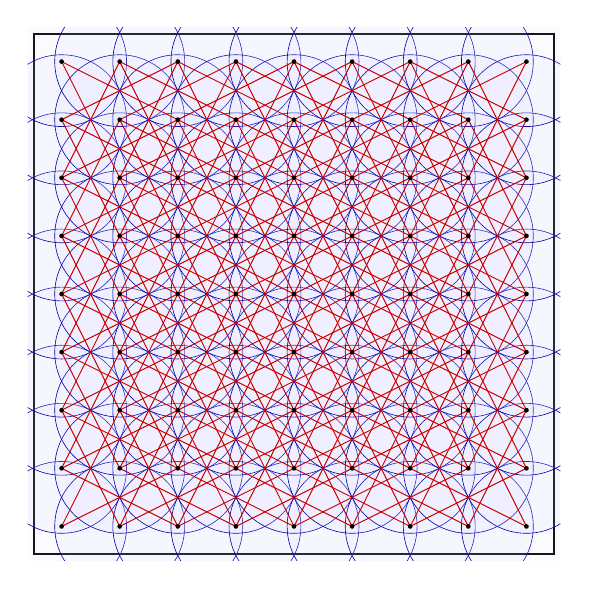
\begin{tikzpicture}[
  scale=1.65,
  halfdisk/.style={draw=blue!65!black, fill=blue!18, fill opacity=0.10, line width=0.22pt},
  unit/.style={draw=red!78!black, line width=0.35pt},
  pt/.style={circle, fill=black, inner sep=0.60pt},
  boundary/.style={draw=black, line width=0.55pt}
]
  \clip (-2.05,-2.05) rectangle (2.05,2.05);
  \draw[boundary] (-2,-2) rectangle (2,2);
  % This is exactly the same scaled lattice as in Figure~\ref{fig:multidirectional-lattice-0-10},
  % restricted to the smaller window [-2,2]^2.
  \foreach \i in {-4,-3,-2,-1,0,1,2,3,4} {
    \foreach \j in {-4,-3,-2,-1,0,1,2,3,4} {
      \pgfmathsetmacro{\x}{0.4472135955*\i}
      \pgfmathsetmacro{\y}{0.4472135955*\j}
      \ifdim \x pt > -2.0001pt
        \ifdim \x pt < 2.0001pt
          \ifdim \y pt > -2.0001pt
            \ifdim \y pt < 2.0001pt
              \draw[halfdisk] (\x,\y) circle[radius=0.5];
            \fi
          \fi
        \fi
      \fi
    }
  }
  % Draw each undirected unit edge once.  The four positive-x displacement
  % representatives (1,2), (1,-2), (2,1), and (2,-1) match the full figure.
  \foreach \i in {-4,-3,-2,-1,0,1,2,3} {
    \foreach \j in {-4,-3,-2,-1,0,1,2} {
      \pgfmathsetmacro{\xA}{0.4472135955*\i}
      \pgfmathsetmacro{\yA}{0.4472135955*\j}
      \pgfmathsetmacro{\xB}{0.4472135955*(\i+1)}
      \pgfmathsetmacro{\yB}{0.4472135955*(\j+2)}
      \ifdim \xA pt > -2.0001pt \ifdim \xA pt < 2.0001pt \ifdim \yA pt > -2.0001pt \ifdim \yA pt < 2.0001pt
      \ifdim \xB pt > -2.0001pt \ifdim \xB pt < 2.0001pt \ifdim \yB pt > -2.0001pt \ifdim \yB pt < 2.0001pt
        \draw[unit] (\xA,\yA) -- (\xB,\yB);
      \fi\fi\fi\fi \fi\fi\fi\fi
    }
  }
  \foreach \i in {-4,-3,-2,-1,0,1,2,3} {
    \foreach \j in {-2,-1,0,1,2,3,4} {
      \pgfmathsetmacro{\xA}{0.4472135955*\i}
      \pgfmathsetmacro{\yA}{0.4472135955*\j}
      \pgfmathsetmacro{\xB}{0.4472135955*(\i+1)}
      \pgfmathsetmacro{\yB}{0.4472135955*(\j-2)}
      \ifdim \xA pt > -2.0001pt \ifdim \xA pt < 2.0001pt \ifdim \yA pt > -2.0001pt \ifdim \yA pt < 2.0001pt
      \ifdim \xB pt > -2.0001pt \ifdim \xB pt < 2.0001pt \ifdim \yB pt > -2.0001pt \ifdim \yB pt < 2.0001pt
        \draw[unit] (\xA,\yA) -- (\xB,\yB);
      \fi\fi\fi\fi \fi\fi\fi\fi
    }
  }
  \foreach \i in {-4,-3,-2,-1,0,1,2} {
    \foreach \j in {-4,-3,-2,-1,0,1,2,3} {
      \pgfmathsetmacro{\xA}{0.4472135955*\i}
      \pgfmathsetmacro{\yA}{0.4472135955*\j}
      \pgfmathsetmacro{\xB}{0.4472135955*(\i+2)}
      \pgfmathsetmacro{\yB}{0.4472135955*(\j+1)}
      \ifdim \xA pt > -2.0001pt \ifdim \xA pt < 2.0001pt \ifdim \yA pt > -2.0001pt \ifdim \yA pt < 2.0001pt
      \ifdim \xB pt > -2.0001pt \ifdim \xB pt < 2.0001pt \ifdim \yB pt > -2.0001pt \ifdim \yB pt < 2.0001pt
        \draw[unit] (\xA,\yA) -- (\xB,\yB);
      \fi\fi\fi\fi \fi\fi\fi\fi
    }
  }
  \foreach \i in {-4,-3,-2,-1,0,1,2} {
    \foreach \j in {-3,-2,-1,0,1,2,3,4} {
      \pgfmathsetmacro{\xA}{0.4472135955*\i}
      \pgfmathsetmacro{\yA}{0.4472135955*\j}
      \pgfmathsetmacro{\xB}{0.4472135955*(\i+2)}
      \pgfmathsetmacro{\yB}{0.4472135955*(\j-1)}
      \ifdim \xA pt > -2.0001pt \ifdim \xA pt < 2.0001pt \ifdim \yA pt > -2.0001pt \ifdim \yA pt < 2.0001pt
      \ifdim \xB pt > -2.0001pt \ifdim \xB pt < 2.0001pt \ifdim \yB pt > -2.0001pt \ifdim \yB pt < 2.0001pt
        \draw[unit] (\xA,\yA) -- (\xB,\yB);
      \fi\fi\fi\fi \fi\fi\fi\fi
    }
  }
  \foreach \i in {-4,-3,-2,-1,0,1,2,3,4} {
    \foreach \j in {-4,-3,-2,-1,0,1,2,3,4} {
      \pgfmathsetmacro{\x}{0.4472135955*\i}
      \pgfmathsetmacro{\y}{0.4472135955*\j}
      \ifdim \x pt > -2.0001pt
        \ifdim \x pt < 2.0001pt
          \ifdim \y pt > -2.0001pt
            \ifdim \y pt < 2.0001pt
              \node[pt] at (\x,\y) {};
            \fi
          \fi
        \fi
      \fi
    }
  }
\end{tikzpicture}
\caption{Local view of the same multidirectional lattice as in Figure~\ref{fig:multidirectional-lattice-0-10}, restricted to the window $[-2,2]^2$.  The points lie on the scaled integer grid $(i/\sqrt5,j/\sqrt5)$, the disks have radius $1/2$, and the red segments show all unit-distance pairs coming from the displacement vectors $(\pm1,\pm2)$ and $(\pm2,\pm1)$.}
\label{fig:multidirectional-lattice-local}
\end{figure}





\section{A nonlinear integer-programming formulation}\label{sec:integer-programming}

The explicit lower-bound criterion suggests the following finite parameter-selection problem.  In computational form it is naturally viewed as a nonlinear integer programming problem with arithmetic feasibility constraints.  One chooses:
\begin{itemize}
  \item a finite set $T$ of odd primes;
  \item a finite set $S_Q$ of rational primes;
  \item integer multiplicities $k(p)\geq 1$ for $p\in S_Q$;
  \item a real parameter $R>1$.
\end{itemize}

For the implementation discussed below, define
\[
  e(p)=
  \begin{cases}
  2, & p=2\text{ or }p\in T,\\
  1, & \text{otherwise.}
  \end{cases}
\]
The exponent-gain objective used in the verification is
\begin{align}
\delta(T,S_Q,k,R)&=\frac{N(T,S_Q,k,R)}{D(T,S_Q,k,R)},\label{eq:delta-objective}\\
N(T,S_Q,k,R)&=\log(1-1/R)+\frac12\log(2\pi/e)\notag\\
&\quad+\sum_{p\in S_Q}\frac{1}{4e(p)}\log(k(p)+1)
-\frac18\log\!\left(4\prod_{q\in T}q\right)\notag\\
&\quad-\frac12\log\!\log\!\sqrt{4\prod_{q\in T}q},\notag\\
D(T,S_Q,k,R)&=\log\!\left(2R\prod_{p\in S_Q}p^{k(p)/(2e(p))}+1\right).\notag
\end{align}
The resulting optimization problem is to maximize $\delta(T,S_Q,k,R)$ subject to arithmetic side conditions.  The optimization stage uses a lightweight admissibility model to generate candidates; the candidate reported in Appendix~\ref{app:verification} is then checked separately by exact integer arithmetic for the side conditions implemented in the verification pipeline.

\section{Heuristic optimization strategies}\label{sec:heuristics}

The finite certificate problem can be read as a nonlinear integer optimization problem with arithmetic feasibility constraints.  The variables are the selected prime set $S_Q$, the integer multiplicities $k(p)$, and the rationally represented real parameter $R$.  The role of the optimization algorithms in this paper is to propose candidate certificates; every reported candidate is then checked independently by the verification pipeline described in Appendix~\ref{app:algorithmic-details} and Appendix~\ref{app:verification}.

This section gives only the main algorithmic ideas.  The precise pseudocode, default parameter values, repair rules, and verification loop are collected in Appendix~\ref{app:algorithmic-details}; the numerical certificate checks are recorded in Appendix~\ref{app:verification}.

\subsection{Greedy budget heuristic}\label{subsec:greedy-heuristic}

The deterministic greedy baseline starts from the Golod--Shafarevich-type side condition
\[
  \#T+\#S_Q+\#\{p\in S_Q:p\text{ splits in }Q\}+1
  \leq \frac{(\#T-1)^2}{4},
\]
where $Q=\mathbb{Q}\!\left(\sqrt{\prod_{q\in T}q}\right)$ in the simplified quadratic-field picture.  This inequality suggests a knapsack interpretation: a non-splitting prime costs one unit of budget, while a splitting prime costs two.  For a provisional target exponent $c$, the greedy construction assigns the approximate multiplicity
\[
  k(p)\approx \left\lfloor \frac{1}{2c\log p}-1\right\rfloor,
  \qquad
  R\approx 1+\frac{1}{c},
\]
and ranks admissible primes by
\[
  \operatorname{score}(p)=
  \frac{\frac{1}{4e(p)}\log(k(p)+1)}{\operatorname{cost}(p)}.
\]
It then fills the available budget in decreasing score order and finally scans a grid of $R$ values.  Figure~\ref{fig:optimization-flow} summarizes this greedy construction: the dashed frame is the budgeted selection of $S_Q$, while the lower part of the diagram represents the subsequent scan over $R$ and evaluation of $\delta(T,S_Q,k,R)$.

The default greedy run used in the implementation fixes $T$ to Sawin's published prime set, uses candidate primes up to $p_{\max}=300$, sets the provisional target to $c=0.015$, and scans $R\in[40,90]$ on a uniform grid with 500 intervals.  These parameter choices are not part of the theorem; they define a reproducible baseline optimization run.  More detailed algorithmic specifications and verification steps are deferred to Appendix~\ref{app:algorithmic-details}.

\begin{figure}[htbp]
\centering
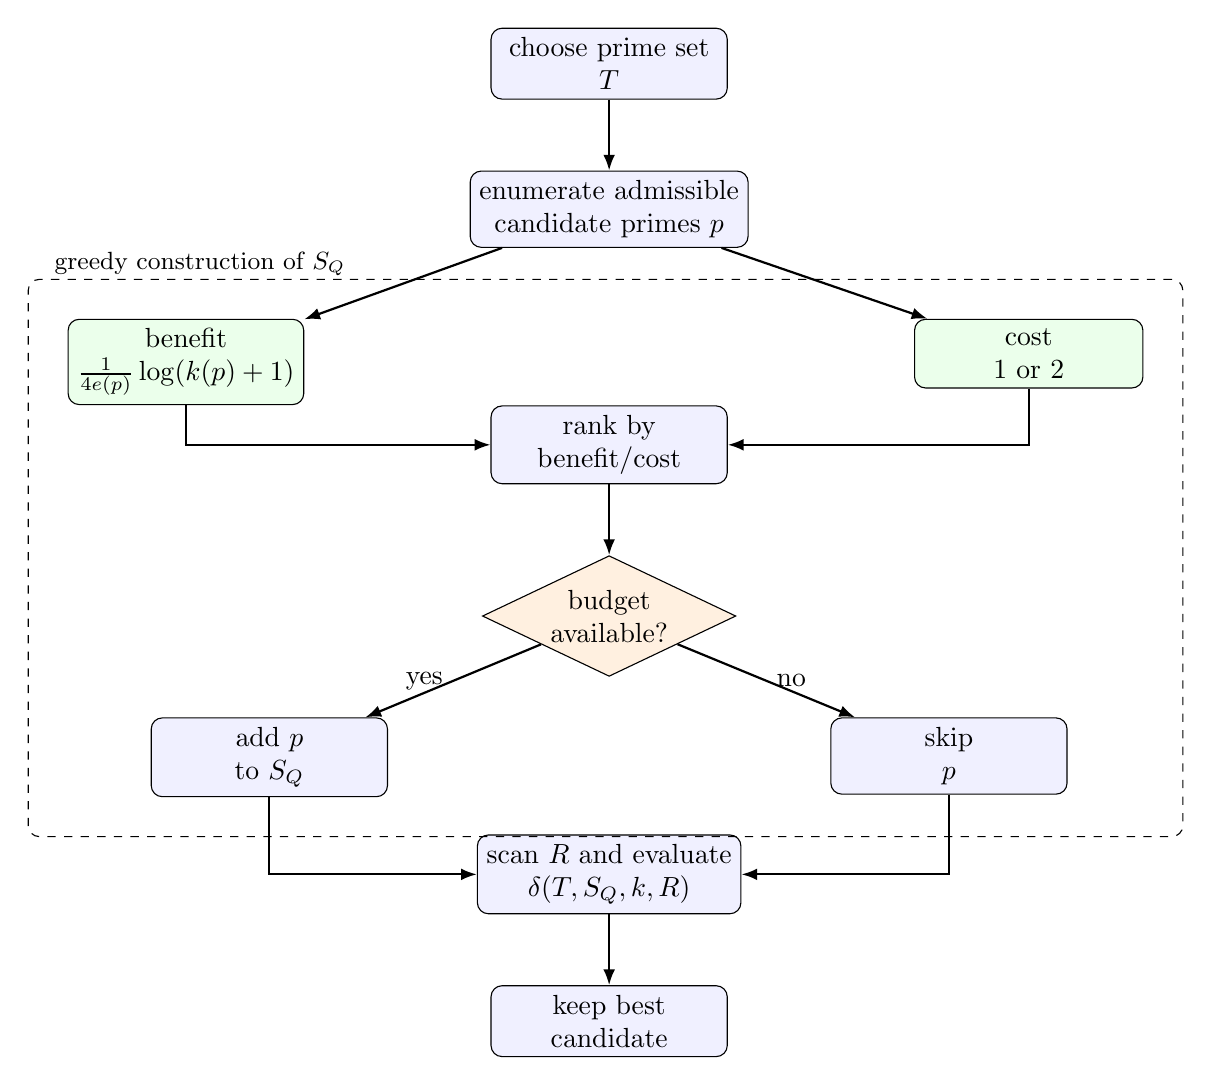
\begin{tikzpicture}[
  node distance=9mm and 9mm,
  box/.style={draw, rounded corners, align=center, minimum height=9mm, minimum width=30mm, fill=blue!6},
  smallbox/.style={draw, rounded corners, align=center, minimum height=8mm, minimum width=29mm, fill=green!8},
  decision/.style={draw, diamond, aspect=2.1, align=center, fill=orange!12, inner sep=1.5pt},
  line/.style={-{Latex[length=2mm]}, thick},
  softline/.style={-{Latex[length=2mm]}, thick, dashed, color=gray!70!black}
]

\node[box] (T) {choose prime set\\$T$};
\node[box, below=of T] (candidates) {enumerate admissible\\candidate primes $p$};
\node[smallbox, below left=of candidates, xshift=-12mm] (benefit) {benefit\\$\frac{1}{4e(p)}\log(k(p)+1)$};
\node[smallbox, below right=of candidates, xshift=12mm] (cost) {cost\\$1$ or $2$};
\node[box, below=20mm of candidates] (score) {rank by\\benefit/cost};
\node[decision, below=of score] (budget) {budget\\available?};
\node[box, below left=of budget, xshift=-11mm] (add) {add $p$\\to $S_Q$};
\node[box, below right=of budget, xshift=11mm] (skip) {skip\\$p$};
\node[box, below=20mm of budget] (scanR) {scan $R$ and evaluate\\$\delta(T,S_Q,k,R)$};
\node[box, below=of scanR] (best) {keep best\\candidate};

\draw[line] (T) -- (candidates);
\draw[line] (candidates) -- (benefit);
\draw[line] (candidates) -- (cost);
\draw[line] (benefit) |- (score);
\draw[line] (cost) |- (score);
\draw[line] (score) -- (budget);
\draw[line] (budget) -- node[left] {yes} (add);
\draw[line] (budget) -- node[right] {no} (skip);
\draw[line] (add.south) |- (scanR.west);
\draw[line] (skip.south) |- (scanR.east);
\draw[line] (scanR) -- (best);

\node[draw, dashed, rounded corners, fit=(benefit)(cost)(score)(budget)(add)(skip), inner sep=5mm] (greedybox) {};
\node[anchor=south west, font=\small, fill=white, inner sep=1pt] at ([xshift=3mm]greedybox.north west) {greedy construction of $S_Q$};
\end{tikzpicture}
\caption{A conceptual optimization pattern for selecting $(T,S_Q,k,R)$.}
\label{fig:optimization-flow}

\end{figure}

\subsection{Tailored Integer Evolution Strategy}\label{subsec:integer-es}

The greedy construction changes the certificate in a largely one-pass way.  The second optimization layer therefore treats the certificate variables directly as integer variables and uses a tailored version of the Integer Evolution Strategy \cite{Rudolph1994} for approximating the solution of the nonlinear integer optimization problem.  This is an integer-valued evolution-strategy instantiation in the Rechenberg--Schwefel tradition.  It uses Rudolph's evolutionary algorithm for integer programming as the relevant integer-mutation model based on the $\ell_1$-symmetric double geometric distribution \cite{Rudolph1994}, and augments it with problem-specific repair operators for the certificate constraints.  Candidate solutions encode selected prime indices, multiplicities, and the numerator $r$ of a rational representation $R=r/s$ with fixed denominator $s$.

The mutation operator is integer-native: it adds two-sided geometric, or discrete-Laplace, steps to integer components instead of mutating real variables and rounding them.  The best reported variant also uses two-parent discrete recombination, where each integer component of an offspring is inherited from one of two parents before mutation.  Since arbitrary mutations can violate the number-theoretic certificate constraints, the implementation augments the integer ES with problem-specific repair operators.  These repairs enforce distinct selected primes, admissible multiplicities, the permitted range for $R$, and the Golod--Shafarevich budget before the objective is evaluated.

The main-text role of this Tailored Integer Evolution Strategy is simple: it optimizes coordinated integer changes that the greedy budget rule is unlikely to find.  The reported single run used a deliberately modest compute budget: population size $\mu=24$, offspring number $\lambda=144$, and $G=160$ generations, corresponding to $24+160\cdot144=23064$ objective-function evaluations, before final verification.  This run completed in less than ten minutes on standard laptop/desktop hardware in the intended reproducibility setting.  Detailed parameters, random seeds, repair rules, and the exact verification loop are specified in Algorithm~\ref{alg:rudolph-discrete-recombination} in Appendix~\ref{app:algorithmic-details}.  The verified certificate produced by this optimization procedure is reported together with the Sawin and greedy certificates in Section~\ref{sec:three-bounds}.

\section{Comparison of verified certificate levels}\label{sec:three-bounds}

The verification pipeline is used in four roles.  It first reproduces Sawin's published explicit certificate as a validation target.  It then checks the greedy certificate, the Tailored integer-ES certificate, and the discrete-recombination variant.  The purpose of this section is only to compare the verified certificate values; the algorithmic details are referenced back to Section~\ref{sec:heuristics} and Appendix~\ref{app:algorithmic-details}.


\begin{table}[htbp]
\centering
\tiny
\begin{tabular}{p{0.28\linewidth}p{0.24\linewidth}p{0.14\linewidth}p{0.20\linewidth}}
\toprule
entry & role & $R$ & exponent parameter $\delta$ \\
\midrule
Sawin published example & validation baseline & $72$ & $0.0141144286784982\ldots$ \\
greedy optimized certificate & deterministic improvement & $66.72240803$ & $0.0151718056372133\ldots$ \\
Tailored integer ES certificate & integer evolutionary improvement & $6672416/100000$ & $0.0152616610684193\ldots$ \\
Tailored integer ES with discrete recombination & recombination variant & $6672416/100000$ & $0.0152628688170072\ldots$ \\
\bottomrule
\end{tabular}
\caption{Verified asymptotic certificate levels. Each row passes the implemented arithmetic checks.}
\label{tab:three-bounds}
\end{table}

\begin{figure}[htbp]
\centering
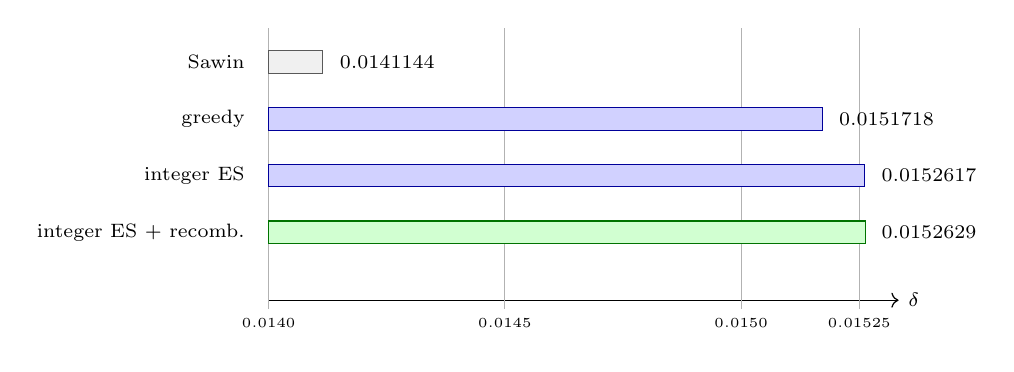
\begin{tikzpicture}[
  xscale=1.0, yscale=0.72,
  bar/.style={draw=blue!60!black, fill=blue!18, line width=0.45pt},
  bestbar/.style={draw=green!45!black, fill=green!18, line width=0.55pt},
  base/.style={draw=gray!70!black, fill=gray!12, line width=0.45pt},
  lab/.style={font=\scriptsize, anchor=east},
  val/.style={font=\scriptsize, anchor=west},
  tick/.style={draw=gray!60, line width=0.3pt}
]
  % Horizontal scale: x = 6000*(delta - 0.014).
  \draw[->, line width=0.45pt] (0,-0.95) -- (8.0,-0.95) node[anchor=west, font=\scriptsize] {$\delta$};
  \foreach \x/\label in {0/0.0140,3/0.0145,6/0.0150,7.5/0.01525} {
    \draw[tick] (\x,-1.10) -- (\x,3.85);
    \node[font=\tiny, anchor=north] at (\x,-1.10) {$\label$};
  }
  \node[lab] at (-0.18,3.25) {Sawin};
  \draw[base] (0,3.05) rectangle (0.6866,3.45);
  \node[val] at (0.78,3.25) {$0.0141144$};

  \node[lab] at (-0.18,2.25) {greedy};
  \draw[bar] (0,2.05) rectangle (7.0308,2.45);
  \node[val] at (7.12,2.25) {$0.0151718$};

  \node[lab] at (-0.18,1.25) {integer ES};
  \draw[bar] (0,1.05) rectangle (7.56997,1.45);
  \node[val] at (7.66,1.25) {$0.0152617$};

  \node[lab] at (-0.18,0.25) {integer ES + recomb.};
  \draw[bestbar] (0,0.05) rectangle (7.57721,0.45);
  \node[val] at (7.66,0.25) {$0.0152629$};

  \node[font=\tiny, anchor=west] at (0,-1.55) {};
\end{tikzpicture}
\caption{Visual comparison of the verified certificate levels.  The horizontal scale is clipped at $\delta=0.014$ so that the differences between the improved certificates remain visible.  The final row is the best certificate found in the recorded computations.}
\label{fig:certificate-comparison}
\end{figure}

The numerical ordering in Table~\ref{tab:three-bounds} and Figure~\ref{fig:certificate-comparison} is the main computational outcome of this version of the report.  Parameter-dashboard visualizations for the Sawin, greedy, and best discrete-recombination certificates are collected in Appendix~\ref{app:verification}; they are displayed in Figures~\ref{fig:sawin-dashboard}, \ref{fig:verified-candidate-dashboard}, and \ref{fig:recomb-candidate-dashboard}.  The greedy optimization already improves the displayed exponent of the validation baseline.  The Tailored Integer Evolution Strategy then improves the greedy certificate by allowing coordinated integer changes in the selected prime set, in the multiplicities $k(p)$, and in the rational representation of $R$.  The discrete-recombination variant gives a further small improvement in this run.  The best current clean consequence supported by the implemented checks is therefore the conservative statement for arbitrarily large $n$:
\[
  u(n)>n^{1.0152}
\]



\section{Reproducible implementation}\label{sec:reproducible-implementation}

The implementations used in this paper are provided at
\begin{center}
\url{https://github.com/emmerichmtm/UnitDistanceProblemOptimizationOfSawinsLowerBound}.
\end{center}
The repository is intended to make the objective function, the verification pipeline, and the optimization heuristics easy to inspect and rerun.  The first recommended command is the verifier:
\begin{verbatim}
python verify_all_certificates_v23.py
\end{verbatim}
It recomputes the finite arithmetic checks for the reported certificates: primality, the parity condition on $T$, Legendre-symbol witnesses, non-splitting of the primes in $S_Q$, the Golod--Shafarevich budget, positivity of the multiplicities, $R>1$, and the value of formula~\eqref{eq:delta-objective}.  The output is written as both text and JSON summaries.

The two optimization scripts are deliberately separated.  The deterministic baseline is the greedy strategy of Section~\ref{subsec:greedy-heuristic}:
\begin{verbatim}
python optimize_certificates.py
\end{verbatim}
The improved optimization method is the Tailored Integer Evolution Strategy with discrete recombination from Section~\ref{subsec:integer-es}:
\begin{verbatim}
python rudolph_integer_es_discrete_recombination.py
\end{verbatim}
The reported evolutionary run uses $23064$ objective-function evaluations in a single run and was kept below ten minutes on standard hardware to make reproduction realistic.  Full command-line options, generated file names, and additional usage notes are maintained in the README; Section~\ref{sec:reproducible-implementation} records only the essential commands, while Appendix~\ref{app:algorithmic-details} records the algorithmic parameters and Appendix~\ref{app:verification} records the certificate-level results.

\section{Outlook and future work}\label{sec:outlook}

The computations reported here suggest several directions for further improvement.  First, the present optimization fixes the same set $T$ used in Sawin's explicit example and explores the induced nonlinear integer-programming problem over $S_Q$, the multiplicities $k(p)$, and a rational representation of $R$.  A natural next step is to enlarge the optimization over $T$ itself, including local exchanges of primes and larger candidate pools.  Second, the lightweight greedy and evolutionary pipelines could be complemented by branch-and-bound, mixed-integer nonlinear programming heuristics, surrogate models, or hybrid local optimization.  Third, the numerical certificate checks should be reproduced with formal interval arithmetic and, ideally, with independent SageMath or Magma verification of the arithmetic side conditions.

There is also a broader theoretical target.  Sawin's paper does not merely provide the explicit lower bound used here; it also discusses limitations and upper bounds for the exponent values obtainable by the same general argument.  The best certificate found in the present computations, $\delta=0.0152628688\ldots$, improves Sawin's displayed explicit value but remains below the upper range discussed for this method.  Thus the computational optimization space has not been exhausted.  Further improvements may come either from better parameter optimization within Sawin's criterion or from strengthening the underlying number-theoretic estimates and field-construction ingredients.

Finally, the present work remains certificate-level.  Producing a concrete coordinate realization of one of the improved asymptotic certificates would require an explicit finite level of the relevant class-field tower, computable algebraic bases, embeddings, ideals, and a projection/windowing procedure.  That remains a separate and more demanding computational number-theory project.


\section{Conclusion}\label{sec:conclusion}

This report has treated the optimization of improved explicit parameters in Sawin's lower-bound criterion as a nonlinear integer optimization problem.  The optimization variables are the selected primes $S_Q$, their integer multiplicities $k(p)$, and a rational representation of the parameter $R$, subject to arithmetic admissibility and Golod--Shafarevich budget constraints.  The implementation first validates the objective and verification pipeline by reproducing Sawin's published certificate with
\[
  \delta=0.0141144286784982\ldots,
\]
and then applies deterministic greedy optimization and the Tailored Integer Evolution Strategy to the same finite certificate problem.

The best certificate found in the reported computations is obtained by a Tailored Integer Evolution Strategy with discrete recombination.  It has
\[
  \delta=0.0152628688170072\ldots,
\]
passes the implemented arithmetic checks, and supports the clean conservative statement
\[
  u(n)>n^{1.0152}
\]
for arbitrarily large $n$, under the same certificate interpretation used throughout this paper.  This improves the displayed clean exponent $1.014$ associated with Sawin's explicit parameter choice at the level of verified finite certificate selection.  The result is not a coordinate construction of the corresponding asymptotic planar point sets; the distinction between certificate verification, coordinate realization, and regular-lattice visualizations is maintained throughout the paper.

The main contribution is therefore computational and methodological: a state-of-the-art but lightweight integer heuristic, adapted to the nonlinear integer structure of Sawin's certificate model, can find a better explicit certificate than the initial hand-selected one.  The accompanying verification scripts make the certificate checks reproducible, while the regular-lattice figures serve only as explanatory visual material for the unit-distance relation and should not be confused with the algebraic certificate construction.

There remains clear room for further optimization.  More concretely, Proposition~15 in \cite{Sawin2026} gives an abstract upper bound of
\[
  1+\frac{1}{4.116}=1.24295\ldots
\]
for the exponent obtainable from the formulation considered there.  The present certificate is therefore still far below the theoretical ceiling suggested by Sawin's abstraction.

This paper not only establishes a new certificate, but also shows that well-crafted heuristic optimization procedures can contribute to problems in pure mathematics and combinatorial geometry.  Having said so, the paper should also be seen as an invitation to optimize better bounds for this problem, and the openly available implementations of the objective function and verification pipeline can be readily used for this.


\section*{Addendum: enlarged-$T$ budgets and the Cordella communication of 4 June 2026}
\addcontentsline{toc}{section}{Addendum: enlarged-$T$ budgets and the Cordella communication of 4 June 2026}

After publication of v1 of this report, Francesco Cordella shared with the author a draft/report on an enlarged-$T$ Sawin-style certificate and indicated that the result may be recorded here as an addendum \cite{Cordella2026}.  The communication is structurally different from the computations in the main body.  The main-body computations keep the ramified set fixed to Sawin's displayed set $T_{\rm Sawin}$ with $\#T=13$ and optimize $S_Q$, the multiplicities $k(p)$, and the scalar parameter $R$ within that fixed-$T$ setting.  Cordella's communicated candidate instead enlarges the ramified set and reports
\[
  \#T=67,\qquad \#S_Q=1021,\qquad R=33.066458,
\]
with no prime of $S_Q$ splitting in $Q$ and with the Golod--Shafarevich budget saturated as
\[
  67+1021+0+1=1089=(67-1)^2/4.
\]
The reported exponent gain is
\[
  \delta=0.03118533444317659059566\ldots,
\]
and hence, under the same certificate interpretation as in Sawin's explicit criterion, the communicated candidate supports the clean statement $u(n)>n^{1.0311}$ for arbitrarily large $n$.

To clarify the scale of this improvement, I ran a small additional variable-$T$ experiment for suitable budgets $N=\#T$.  The verification script included with the ancillary files chooses the first $N$ odd primes when the parity condition is satisfied, fills the no-split admissible $S_Q$ budget, optimizes integer multiplicities greedily by marginal improvement, and refines $R$ on a grid.  Each plotted rerun is accepted only after passing the finite verification pipeline.  The method is still a lightweight integer-ES/local-search replay, not a formal independent reconstruction of Cordella's full certificate file.  It nevertheless reproduces the qualitative shape of Cordella's communicated plot and gives a value at $N=67$ matching the communicated value to the displayed precision.

\begin{figure}[htbp]
\centering
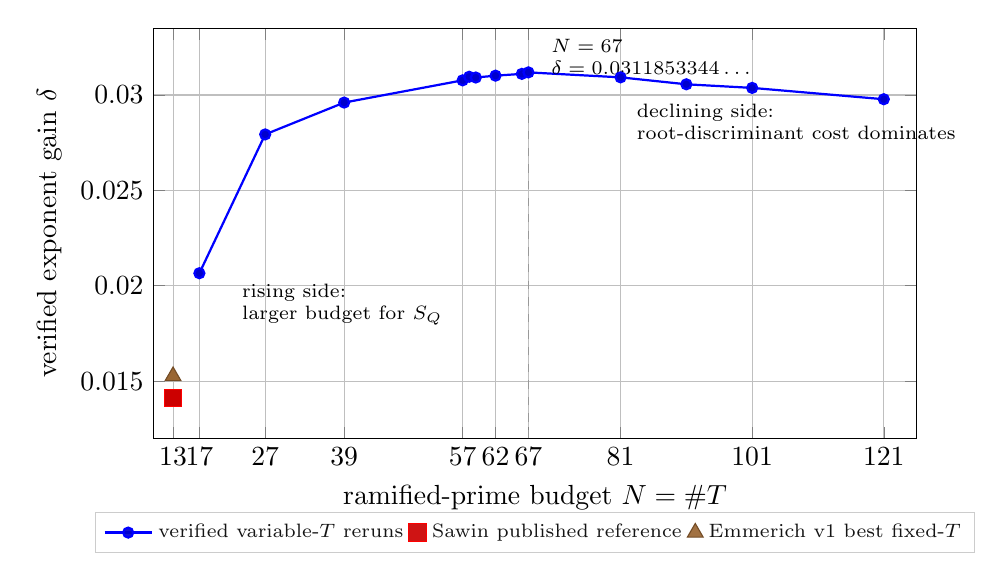
\begin{tikzpicture}
\begin{axis}[
  width=0.93\linewidth,
  height=0.56\linewidth,
  xlabel={ramified-prime budget $N=\#T$},
  ylabel={verified exponent gain $\delta$},
  xmin=10, xmax=126,
  ymin=0.012, ymax=0.0335,
  xtick={13,17,27,39,57,62,67,81,101,121},
  ytick={0.015,0.020,0.025,0.030},
  scaled y ticks=false,
  yticklabel style={/pgf/number format/fixed,/pgf/number format/precision=3},
  grid=both,
  legend columns=3,
  legend style={font=\scriptsize, at={(0.5,-0.18)}, anchor=north, fill=white, fill opacity=0.92, draw=black!20},
  clip=false,
]
\addplot+[mark=*, mark size=1.8pt, thick] coordinates {
  (17,0.020656253147315612)
  (27,0.027933402211705776)
  (39,0.029602831517764342)
  (57,0.030768173984261171)
  (58,0.030956217857676170)
  (59,0.030916033643097813)
  (62,0.031013128415294067)
  (66,0.031106794046674482)
  (67,0.031185334443042398)
  (81,0.030924456853821611)
  (91,0.030560468193505838)
  (101,0.030371856712670109)
  (121,0.029777886451565502)
};
\addlegendentry{verified variable-$T$ reruns}

\addplot+[only marks, mark=square*, mark size=3.2pt] coordinates {(13,0.0141144286784982)};
\addlegendentry{Sawin published reference}

\addplot+[only marks, mark=triangle*, mark size=3.3pt] coordinates {(13,0.0152628688170072)};
\addlegendentry{Emmerich v1 best fixed-$T$}

\draw[dashed, black!40] (axis cs:67,0.012) -- (axis cs:67,0.03118533444317659);
\node[font=\scriptsize, anchor=west, align=left] at (axis cs:69,0.0320)
  {$N=67$\\$\delta=0.0311853344\ldots$};
\node[font=\scriptsize, anchor=west, align=left] at (axis cs:82,0.0286)
  {declining side:\\root-discriminant cost dominates};
\node[font=\scriptsize, anchor=west, align=left] at (axis cs:22,0.0190)
  {rising side:\\larger budget for $S_Q$};
\end{axis}
\end{tikzpicture}
\caption{Budget-dependent exponent values $\delta$ as a function of $N=\#T$.  The square marks Sawin's published fixed-$T$ certificate, the triangle marks the best fixed-$T$ certificate from v1 of the present report, and the connected markers show verified variable-$T$ reruns performed for this addendum.  The rise of the curve is explained by the rapidly growing Golod--Shafarevich budget, which allows many more admissible primes in $S_Q$; the decline beyond the maximum reflects the increasing discriminant cost and denominator growth as $T$ becomes larger.}
\label{fig:addendum-budget-curve}
\end{figure}

\begin{table}[htbp]
\centering
\small
\begin{tabular}{rrrrl}
\toprule
$N=\#T$ & $\#S_Q$ & $R$ & $\delta$ & status/source\\
\midrule
13 & 22 & 72.00 & 0.0141144287 & Sawin published reference\\
13 & 22 & 66.72416 & 0.0152628688 & Emmerich v1 best fixed-$T$\\
17 & 46 & 49.42 & 0.0206562531 & verified variable-$T$ rerun\\
27 & 141 & 36.80 & 0.0279334022 & verified variable-$T$ rerun\\
39 & 321 & 34.78 & 0.0296028315 & verified variable-$T$ rerun\\
57 & 726 & 33.50 & 0.0307681740 & verified variable-$T$ rerun\\
58 & 753 & 33.30 & 0.0309562179 & verified variable-$T$ rerun\\
59 & 781 & 33.34 & 0.0309160336 & verified variable-$T$ rerun\\
62 & 867 & 33.24 & 0.0310131284 & verified variable-$T$ rerun\\
66 & 989 & 33.14 & 0.0311067940 & verified variable-$T$ rerun\\
67 & 1021 & 33.06 & 0.0311853344 & verified variable-$T$ rerun\\
81 & 1518 & 33.34 & 0.0309244569 & verified variable-$T$ rerun\\
91 & 1933 & 33.72 & 0.0305604682 & verified variable-$T$ rerun\\
101 & 2398 & 33.92 & 0.0303718567 & verified variable-$T$ rerun\\
121 & 3478 & 34.58 & 0.0297778865 & verified variable-$T$ rerun\\
\bottomrule
\end{tabular}
\caption{Reference points and additional suitable-budget reruns used in Figure~\ref{fig:addendum-budget-curve}.  Only certificates that passed the verification pipeline are listed.}
\label{tab:addendum-budget-reruns}
\end{table}

The shape of Figure~\ref{fig:addendum-budget-curve} is mathematically plausible.  For small and moderate values of $N=\#T$, enlarging $T$ increases the Golod--Shafarevich budget quadratically, so the optimization can admit many more admissible primes into $S_Q$ and obtain a noticeably stronger positive contribution from the multiplicity term.  After the peak, however, the penalties associated with a larger ramified set become dominant: the discriminant term $-\tfrac18\log(4\prod_{q\in T}q)$ becomes more negative, and the denominator term in the expression for $\delta$ also grows.  The resulting balance naturally produces an initial rise, a broad optimum near the mid-to-high sixties, and a gradual decline afterwards.

For repository-level reproducibility of the enlarged-$T$ addendum, the next required item remains a canonical machine-readable certificate containing the explicit lists of $T$, $S_Q$, the multiplicities $k(p)$, and the value of $R$ for each enlarged-$T$ point.


\appendix
\section{Pseudocode for the Tailored Integer Evolution Strategy and verification pipeline}\label{app:algorithmic-details}

This appendix gives a precise algorithmic description of the Tailored Integer Evolution Strategy used in the implementation.  The notation is adapted to the certificate problem studied in the report.  A chromosome encodes a finite set of selected prime indices, a vector of integer multiplicities, and an integer numerator for the rational representation of $R$.  The denominator of $R$ is fixed, so every optimization variable is integer-valued.  The objective value is the exponent gain $\delta$ from formula~\eqref{eq:delta-objective}, with infeasible certificates receiving value $-\infty$ or being repaired before evaluation.  The values listed in Algorithm~\ref{alg:rudolph-discrete-recombination} are the default parameters used for the reported run.  The initial population contains the published Sawin certificate, the greedy certificate, the best simple integer-ES certificate, and mutated greedy seeds until the population size is reached.

\begin{algorithm}[htbp]
\caption{Tailored Integer Evolution Strategy with discrete recombination}
\label{alg:rudolph-discrete-recombination}
\begin{algorithmic}[1]
\Require fixed prime set $T$; candidate-prime bound $p_{\max}=300$; target size $m=22$; budget bound $B$; population size $\mu=24$; offspring number $\lambda=144$; generation limit $G=160$; random seeds $12345,54321,98765,20260601$; rational denominator $s=100000$ for $R=r/s$; $R$-range $40\le R\le90$; multiplicity bounds $1\le k(p)\le80$; mutation parameters $\alpha_I=0.42$, $\alpha_k=0.35$, $\alpha_R=0.35$, $p_I=0.18$, $p_k=0.35$, $p_R=0.85$
\Ensure best feasible certificate $(T,S_Q,k,R)$ and verified value $\delta$
\State Initialize the pseudorandom generator with the selected seed and initialize a population $P$ of $\mu$ feasible integer chromosomes.
\State Each chromosome has the form $x=(I,k,r)$, where $I$ is a list of $m$ indices into $C$, $k$ is the integer multiplicity vector, and $R=r/s$.
\State Evaluate every $x\in P$ by calling the certificate verifier; store $f(x)=\delta(x)$ if feasible and $f(x)=-\infty$ otherwise.
\For{$g=1,2,\ldots,G$}
  \State Let $E$ be the current elite set, consisting of the best feasible parents in $P$.
  \State Initialize an empty offspring set $O$; use the integer mutation parameters $(\alpha_I,\alpha_k,\alpha_R,p_I,p_k,p_R)$ throughout this generation.
  \For{$j=1,2,\ldots,\lambda$}
    \State Select two parents $x^{(a)}=(I^{(a)},k^{(a)},r^{(a)})$ and $x^{(b)}=(I^{(b)},k^{(b)},r^{(b)})$ from $E$.
    \State \textbf{Discrete recombination:} for each integer component, independently inherit the component from parent $a$ 
    \State $\ $ or parent $b$ with probability $1/2$.
    \State Let the recombined chromosome be $y=(I^{(y)},k^{(y)},r^{(y)})$.
    \State \textbf{Integer-native mutation:} with probability $p_{\rm mut}$ per component, add a two-sided geometric, equivalently \State $\ $ discrete-Laplace, integer step $Z$ to that component.
    \State Repair $y$ by enforcing valid prime indices, distinct selected primes, positive multiplicities, $R>1$, and the \State $\ $Golod--Shafarevich budget.
    \State Evaluate the repaired offspring $y$ using the certificate verifier.
    \State Add $y$ to $O$.
  \EndFor
  \State Set $P$ to the best $\mu$ chromosomes from $P\cup O$ under the objective $f$.
  \State Record the best value at sparse epochs for reproducibility.
\EndFor
\State \Return the best feasible chromosome in the final population.
\end{algorithmic}
\end{algorithm}

\paragraph{Walkthrough.}
The reported run uses $p_{\max}=300$, $m=22$, $\mu=24$, $\lambda=144$, $G=160$, $s=100000$, $40\le R\le90$, and the four random seeds listed above.  Thus a single evolutionary run uses $\mu+G\lambda=24+160\cdot144=23064$ objective-function evaluations, followed by the final verification report.  The optimization starts from feasible certificates, including the published Sawin certificate, the greedy certificate, the best simple integer-ES certificate, and small perturbations of these known good points.  Discrete recombination is used only on integer-coded components: selected-prime indices, multiplicities, and the numerator $r$ in $R=r/s$.  After recombination, integer-valued mutation in the Rudolph tradition changes integer components directly; it does not mutate real-valued variables and then round them.  A repair step keeps the candidate within the admissible optimization space.  Finally, every survivor is checked by the same verification routine used for the reported certificates.  This makes the optimization layer heuristic, but the scoring layer deterministic and reproducible.

The mutation law is the essential Rudolph-style ingredient: the step $Z\in\mathbb Z$ is $\ell_1$ symmetric, centered at zero, and has geometrically decaying tails.  Thus small moves are most frequent, while larger jumps remain possible.  This is appropriate for the present nonlinear integer-programming variant, where changing an optimization variable by a small amount can alter the certificate value, but occasional larger moves help escape local plateaus.

\begin{algorithm}[htbp]
\caption{Certificate verification pipeline}
\label{alg:certificate-verification}
\begin{algorithmic}[1]
\Require candidate data $(T,S_Q,k,R)$
\Ensure pass/fail status and exponent value $\delta$ if all checks pass
\State Check that $T$ consists of odd primes and that the required parity condition on primes $q\equiv 3\pmod 4$ is satisfied.
\State Compute $D=\prod_{q\in T}q$ and set $Q=\mathbb Q(\sqrt D)$ at the level of exact integer arithmetic.
\For{each $p\in S_Q$}
  \State Check primality of $p$ and positivity of $k(p)$.
  \State Compute the Legendre/Kronecker symbols needed to determine whether $p$ is ramified, inert, or split in $Q$.
  \State Check the admissibility condition: $p\equiv 1\pmod 4$ or $p$ is inert in $\mathbb Q(\sqrt q)$ for at least one $q\in T$.
\EndFor
\State Compute the split-prime count $s_Q=\#\{p\in S_Q:p\text{ splits in }Q\}$.
\State Verify the budget inequality
\[
\#T+\#S_Q+s_Q+1\leq \frac{(\#T-1)^2}{4}.
\]
\State Check $R>1$ and evaluate $N(T,S_Q,k,R)$ and $D(T,S_Q,k,R)$ in formula~\eqref{eq:delta-objective} using high-precision decimal arithmetic.
\State Return $\delta=N/D$ together with all diagnostic flags.
\end{algorithmic}
\end{algorithm}

The public implementation of this pipeline is available at
\begin{center}
\url{https://github.com/emmerichmtm/UnitDistanceProblemOptimizationOfSawinsLowerBound}
\end{center}
Algorithm~\ref{alg:certificate-verification} summarizes the verification pipeline.  The verification scripts are meant to be readable reference implementations: they reproduce Sawin's published certificate, the greedy certificate, the Tailored Integer Evolution Strategy certificate, and the discrete-recombination certificate reported in this paper.

\section{Validation of the verification pipeline and verification of the best-found candidate}\label{app:verification}

This appendix records five verification examples based on the explicit criterion used in Sawin's quantitative lower bound \cite{Sawin2026}.  First, the pipeline is run on Sawin's published parameter choice from the proof of Theorem~1, in order to verify that the implementation reproduces the advertised exponent $\delta\approx 0.0141144$.  Second, the same pipeline is applied to the greedy certificate produced by the deterministic optimization procedure.  Third, it is applied to the certificate produced by the Tailored Integer Evolution Strategy.  Fourth, it is applied to the certificate produced by the discrete-recombination variant.  Finally, the appendix records the verified enlarged-$T$ example communicated by Francesco Cordella and now supplied as canonical data.  In all cases, the checked data consist of finite sets $T$ and $S_Q$, integer weights $k(p)$, and a real parameter $R>1$, from which the exponent in formula~\eqref{eq:delta-objective} is computed once the arithmetic side conditions are verified.  The OpenAI announcement and the human-verified remarks explain the broader counterexample and context \cite{OpenAI2026,AlonEtAl2026}.

\subsection*{Validation on Sawin's published parameter choice}

The published example in the proof of Theorem~1 of \cite{Sawin2026} uses
\[
T=\{3,5,7,11,13,17,19,23,29,31,37,41,43\},
\]
with
\[
\begin{split}
S_Q=\{&2,3,5,7,11,13,17,19,23,29,47,71,79,97,101,107,109,139,151,163,167,179\}.
\end{split}
\]
The multiplicities are
\[
\begin{array}{c|rrrrrrrrrrr}
p&2&3&5&7&11&13&17&19&23&29&47\\
\hline
k(p)&50&31&21&17&14&13&12&11&10&10&8
\end{array}
\]
\[
\begin{array}{c|rrrrrrrrrrr}
p&71&79&97&101&107&109&139&151&163&167&179\\
\hline
k(p)&7&7&7&7&7&7&6&6&6&6&6
\end{array}
\]
and
\[
R=72.
\]
The purpose of including this example here is twofold: it validates the implementation against the published reference point, and it illustrates the certificate language before the improved candidate is discussed.

The same arithmetic checks as in the optimized case pass for this published example.  The primes in $T$ are odd, exactly seven of them are congruent to $3\pmod 4$, the set $S_Q$ contains no split primes in $Q=\mathbb{Q}(\sqrt D)$ with $D=\prod_{q\in T}q$, and the Golod--Shafarevich budget is again exactly saturated:
\[
\#T+\#S_Q+\#\{p\in S_Q:p\text{ splits in }Q\}+1=13+22+0+1=36=\frac{(13-1)^2}{4}.
\]
Evaluating formula~\eqref{eq:delta-objective} gives
\[
\text{numerator}=3.8822487482003876\ldots,
\qquad
\text{denominator}=275.0553236430010\ldots,
\]
so that
\[
\delta=0.014114428678498239\ldots,
\]
which reproduces Sawin's printed value $0.014114\ldots$.

\begin{proposition}[Validation against Sawin's published example]
Using the finite data displayed above, the verification pipeline reproduces the explicit lower-bound certificate from the proof of Theorem~1 in \cite{Sawin2026} and confirms the numerical exponent $\delta\approx 0.0141144287$.
\end{proposition}

\subsection*{Graphical description of Sawin's published example}

Figure~\ref{fig:sawin-dashboard} visualizes the published certificate at the parameter level.  It records the set $T$, the selected primes $S_Q$, their multiplicities $k(p)$, and the exact budget saturation.

\begin{figure}[htbp]
\centering
\resizebox{0.98\linewidth}{!}{%
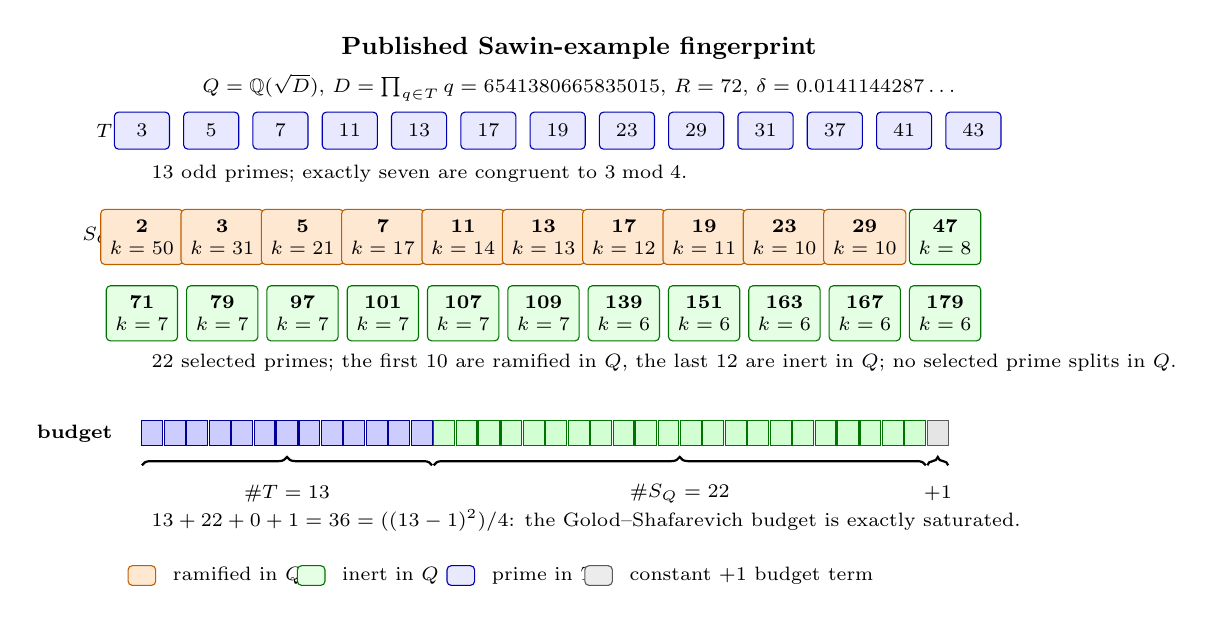
\begin{tikzpicture}[
  font=\scriptsize,
  tcell/.style={draw=blue!70!black, fill=blue!9, rounded corners=1.5pt, minimum width=0.70cm, minimum height=0.47cm, align=center},
  inertcell/.style={draw=green!45!black, fill=green!10, rounded corners=1.5pt, minimum width=0.90cm, minimum height=0.70cm, align=center},
  ramcell/.style={draw=orange!75!black, fill=orange!18, rounded corners=1.5pt, minimum width=0.90cm, minimum height=0.70cm, align=center},
  basecell/.style={draw=gray!70!black, fill=gray!15, rounded corners=1.5pt, minimum width=0.35cm, minimum height=0.25cm, align=center},
  note/.style={align=left, font=\scriptsize},
  lab/.style={font=\scriptsize\bfseries, anchor=east}
]

\node[font=\small\bfseries, align=center] at (5.55,1.05) {Published Sawin-example fingerprint};
\node[note, align=center] at (5.55,0.55) {$Q=\mathbb{Q}(\sqrt{D})$, $D=\prod_{q\in T}q=6541380665835015$, $R=72$, $\delta=0.0141144287\ldots$};

\node[lab] at (-0.25,0) {$T$};
\foreach \p [count=\i from 0] in {3,5,7,11,13,17,19,23,29,31,37,41,43} {
  \node[tcell] at (\i*0.88,0) {\p};
}
\node[note, anchor=west] at (0,-0.55) {13 odd primes; exactly seven are congruent to $3\bmod 4$.};

\node[lab] at (-0.25,-1.35) {$S_Q$};
\foreach \p/\k/\sty [count=\i from 0] in {2/50/ramcell,3/31/ramcell,5/21/ramcell,7/17/ramcell,11/14/ramcell,13/13/ramcell,17/12/ramcell,19/11/ramcell,23/10/ramcell,29/10/ramcell,47/8/inertcell} {
  \node[\sty] at (\i*1.02,-1.35) {\textbf{\p}\\$k=\k$};
}
\foreach \p/\k/\sty [count=\i from 0] in {71/7/inertcell,79/7/inertcell,97/7/inertcell,101/7/inertcell,107/7/inertcell,109/7/inertcell,139/6/inertcell,151/6/inertcell,163/6/inertcell,167/6/inertcell,179/6/inertcell} {
  \node[\sty] at (\i*1.02,-2.32) {\textbf{\p}\\$k=\k$};
}
\node[note, anchor=west] at (0,-2.95) {22 selected primes; the first 10 are ramified in $Q$, the last 12 are inert in $Q$; no selected prime splits in $Q$.};

\node[lab] at (-0.25,-3.85) {budget};
\foreach \i in {0,...,12} {\draw[draw=blue!60!black, fill=blue!20] ({0.285*\i},-4.00) rectangle ++(0.265,0.32);} 
\foreach \i in {13,...,34} {\draw[draw=green!45!black, fill=green!18] ({0.285*\i},-4.00) rectangle ++(0.265,0.32);} 
\draw[draw=gray!70!black, fill=gray!20] ({0.285*35},-4.00) rectangle ++(0.265,0.32);
\draw[decorate, decoration={brace, amplitude=3pt}, thick] (0,-4.25) -- ({0.285*13-0.02},-4.25) node[midway, yshift=-0.36cm] {$\#T=13$};
\draw[decorate, decoration={brace, amplitude=3pt}, thick] ({0.285*13},-4.25) -- ({0.285*35-0.02},-4.25) node[midway, yshift=-0.36cm] {$\#S_Q=22$};
\draw[decorate, decoration={brace, amplitude=3pt}, thick] ({0.285*35},-4.25) -- ({0.285*36-0.02},-4.25) node[midway, yshift=-0.36cm] {$+1$};
\node[note, anchor=west] at (0,-4.95) {$13+22+0+1=36=((13-1)^2)/4$: the Golod--Shafarevich budget is exactly saturated.};

\node[ramcell, minimum width=0.35cm, minimum height=0.25cm] at (0,-5.65) {};
\node[anchor=west] at (0.27,-5.65) {ramified in $Q$};
\node[inertcell, minimum width=0.35cm, minimum height=0.25cm] at (2.15,-5.65) {};
\node[anchor=west] at (2.42,-5.65) {inert in $Q$};
\node[tcell, minimum width=0.35cm, minimum height=0.25cm] at (4.05,-5.65) {};
\node[anchor=west] at (4.32,-5.65) {prime in $T$};
\node[basecell] at (5.80,-5.65) {};
\node[anchor=west] at (6.07,-5.65) {constant $+1$ budget term};
\end{tikzpicture}}
\caption{Parameter-level visualization of Sawin's published explicit example.  The figure is included here as a validation target for the verification pipeline and as a certificate-level illustration of the method.}
\label{fig:sawin-dashboard}
\end{figure}




\subsection*{Greedy optimized candidate from the deterministic optimization}



After the validation run above, the same pipeline was applied to the best candidate found by the optimization procedure.  That candidate is
\[
T=\{3,5,7,11,13,17,19,23,29,31,37,41,43\},
\]
with
\[
\begin{split}
S_Q=\{&2,3,47,71,79,97,101,107,109,139,151,163,167,179,\\
      &191,211,223,239,241,251,257,263\}.
\end{split}
\]
The chosen multiplicities are
\[
\begin{array}{c|rrrrrrrrrrr}
p&2&3&47&71&79&97&101&107&109&139&151\\
\hline
k(p)&47&29&7&6&6&6&6&6&6&5&5
\end{array}
\]
\[
\begin{array}{c|rrrrrrrrrrr}
p&163&167&179&191&211&223&239&241&251&257&263\\
\hline
k(p)&5&5&5&5&5&5&5&5&5&5&4
\end{array}
\]
and the grid-selected value is
\[
R=66.72240803.
\]

\subsection*{Visualization of the verified certificate}

Figure~\ref{fig:verified-candidate-dashboard} visualizes the optimized candidate at the parameter level.  It is not a drawing of the final Euclidean point configuration, whose construction is number-theoretic and asymptotic; rather, it shows the finite certificate data checked by the implementation: the prime set $T$, the selected primes $S_Q$, their multiplicities $k(p)$, and the exact saturation of the Golod--Shafarevich budget.

\begin{figure}[htbp]
\centering
\resizebox{0.98\linewidth}{!}{%
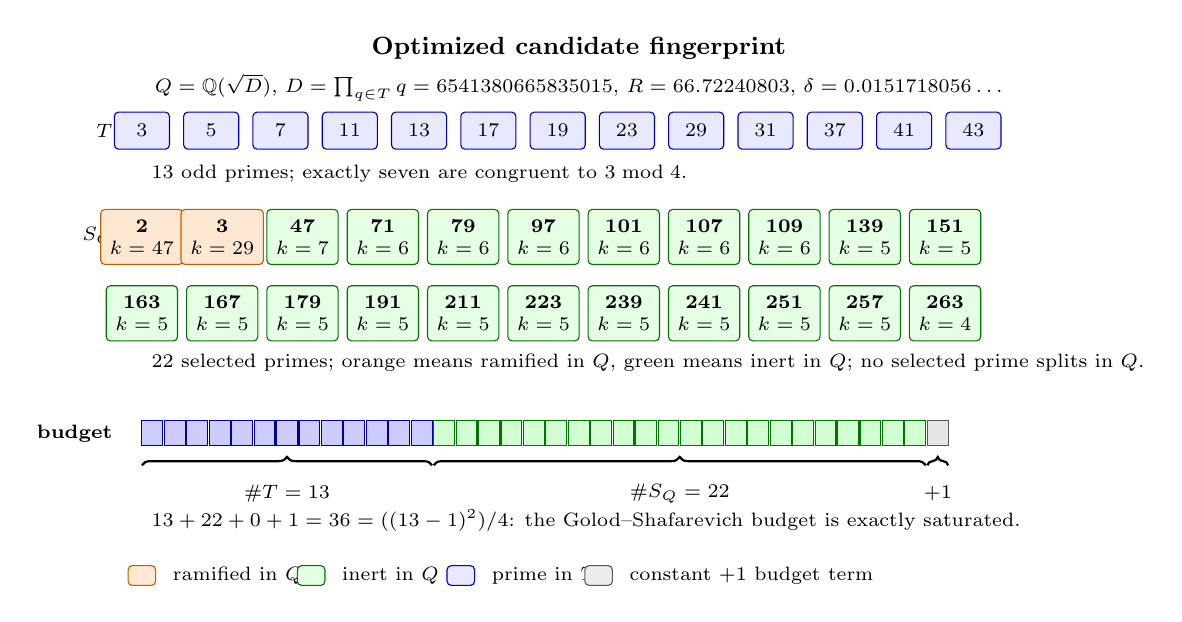
\begin{tikzpicture}[
  font=\scriptsize,
  tcell/.style={draw=blue!70!black, fill=blue!9, rounded corners=1.5pt, minimum width=0.70cm, minimum height=0.47cm, align=center},
  inertcell/.style={draw=green!45!black, fill=green!10, rounded corners=1.5pt, minimum width=0.90cm, minimum height=0.70cm, align=center},
  ramcell/.style={draw=orange!75!black, fill=orange!18, rounded corners=1.5pt, minimum width=0.90cm, minimum height=0.70cm, align=center},
  basecell/.style={draw=gray!70!black, fill=gray!15, rounded corners=1.5pt, minimum width=0.35cm, minimum height=0.25cm, align=center},
  note/.style={align=left, font=\scriptsize},
  lab/.style={font=\scriptsize\bfseries, anchor=east}
]

\node[font=\small\bfseries, align=center] at (5.55,1.05) {Optimized candidate fingerprint};
\node[note, align=center] at (5.55,0.55) {$Q=\mathbb{Q}(\sqrt{D})$, $D=\prod_{q\in T}q=6541380665835015$, $R=66.72240803$, $\delta=0.0151718056\ldots$};

% T row.
\node[lab] at (-0.25,0) {$T$};
\foreach \p [count=\i from 0] in {3,5,7,11,13,17,19,23,29,31,37,41,43} {
  \node[tcell] at (\i*0.88,0) {\p};
}
\node[note, anchor=west] at (0,-0.55) {13 odd primes; exactly seven are congruent to $3\bmod 4$.};

% S_Q rows.
\node[lab] at (-0.25,-1.35) {$S_Q$};
\foreach \p/\k/\sty [count=\i from 0] in {2/47/ramcell,3/29/ramcell,47/7/inertcell,71/6/inertcell,79/6/inertcell,97/6/inertcell,101/6/inertcell,107/6/inertcell,109/6/inertcell,139/5/inertcell,151/5/inertcell} {
  \node[\sty] at (\i*1.02,-1.35) {\textbf{\p}\\$k=\k$};
}
\foreach \p/\k/\sty [count=\i from 0] in {163/5/inertcell,167/5/inertcell,179/5/inertcell,191/5/inertcell,211/5/inertcell,223/5/inertcell,239/5/inertcell,241/5/inertcell,251/5/inertcell,257/5/inertcell,263/4/inertcell} {
  \node[\sty] at (\i*1.02,-2.32) {\textbf{\p}\\$k=\k$};
}
\node[note, anchor=west] at (0,-2.95) {22 selected primes; orange means ramified in $Q$, green means inert in $Q$; no selected prime splits in $Q$.};

% Budget bar.
\node[lab] at (-0.25,-3.85) {budget};
\foreach \i in {0,...,12} {
  \draw[draw=blue!60!black, fill=blue!20] ({0.285*\i},-4.00) rectangle ++(0.265,0.32);
}
\foreach \i in {13,...,34} {
  \draw[draw=green!45!black, fill=green!18] ({0.285*\i},-4.00) rectangle ++(0.265,0.32);
}
\draw[draw=gray!70!black, fill=gray!20] ({0.285*35},-4.00) rectangle ++(0.265,0.32);
\draw[decorate, decoration={brace, amplitude=3pt}, thick] (0,-4.25) -- ({0.285*13-0.02},-4.25) node[midway, yshift=-0.36cm] {$\#T=13$};
\draw[decorate, decoration={brace, amplitude=3pt}, thick] ({0.285*13},-4.25) -- ({0.285*35-0.02},-4.25) node[midway, yshift=-0.36cm] {$\#S_Q=22$};
\draw[decorate, decoration={brace, amplitude=3pt}, thick] ({0.285*35},-4.25) -- ({0.285*36-0.02},-4.25) node[midway, yshift=-0.36cm] {$+1$};
\node[note, anchor=west] at (0,-4.95) {$13+22+0+1=36=((13-1)^2)/4$: the Golod--Shafarevich budget is exactly saturated.};

% Legend.
\node[ramcell, minimum width=0.35cm, minimum height=0.25cm] at (0,-5.65) {};
\node[anchor=west] at (0.27,-5.65) {ramified in $Q$};
\node[inertcell, minimum width=0.35cm, minimum height=0.25cm] at (2.15,-5.65) {};
\node[anchor=west] at (2.42,-5.65) {inert in $Q$};
\node[tcell, minimum width=0.35cm, minimum height=0.25cm] at (4.05,-5.65) {};
\node[anchor=west] at (4.32,-5.65) {prime in $T$};
\node[basecell] at (5.80,-5.65) {};
\node[anchor=west] at (6.07,-5.65) {constant $+1$ budget term};
\end{tikzpicture}}
\caption{Parameter-level visualization of the optimized candidate in Appendix~\ref{app:verification}. The colored budget bar shows exact saturation of the side condition: 13 slots for $T$, 22 slots for $S_Q$, no split-prime penalty, and one constant slot.}
\label{fig:verified-candidate-dashboard}
\end{figure}

\subsection*{Coordinate-realization scope}

The dashboard figures in this appendix visualize finite certificate data, not Euclidean coordinates of the asymptotic point sets.  A literal coordinate realization of an optimized certificate would require additional number-theoretic data not specified by $(T,S_Q,k,R)$: an explicit finite level of the relevant class-field tower, algebraic bases or defining polynomials, ideals, embeddings, normalization, and a bounded planar window.  The present implementation therefore focuses on parameter optimization and certificate verification.  Constructing such coordinates remains a separate computational number-theory project.

\subsection*{Arithmetic checks}

Let
\(
D=\prod_{q\in T}q=6541380665835015,
\qquad
Q=\mathbb{Q}(\sqrt D).
\)
The set $T$ consists of odd primes and exactly seven of its elements are congruent to $3\pmod 4$, so the required parity condition is satisfied.  The verification checks, using exact integer arithmetic and Legendre-symbol computations, that every prime in $S_Q$ is either ramified or inert in $Q$; none is split.  Thus
\[
\#\{p\in S_Q:p\text{ splits in }Q\}=0.
\]
The Golod--Shafarevich budget side condition therefore becomes
\[
\#T+\#S_Q+\#\{p\in S_Q:p\text{ splits in }Q\}+1
=13+22+0+1=36, \mbox{while}
\]
\[
\frac{(\#T-1)^2}{4}=\frac{12^2}{4}=36.
\]
Hence the budget is exactly saturated.

For admissibility in Sawin's Lemma~12, each $p\in S_Q$ must be congruent to $1\pmod 4$ or inert in $\mathbb{Q}(\sqrt q)$ for some $q\in T$.  The verification script found the following witnesses.

\begin{center}
\scriptsize
\begin{tabular}{rll}
\toprule
$p$ & status in $Q$ & admissibility witness \\
\midrule
2   & ramified & inert in $\mathbb{Q}(\sqrt5)$ \\
3   & ramified & inert in $\mathbb{Q}(\sqrt5)$ \\
47  & inert & inert in $\mathbb{Q}(\sqrt5)$ \\
71  & inert & inert in $\mathbb{Q}(\sqrt7)$ \\
79  & inert & inert in $\mathbb{Q}(\sqrt3)$ \\
97  & inert & $p\equiv1\pmod4$ \\
101 & inert & $p\equiv1\pmod4$ \\
107 & inert & inert in $\mathbb{Q}(\sqrt5)$ \\
109 & inert & $p\equiv1\pmod4$ \\
139 & inert & inert in $\mathbb{Q}(\sqrt3)$ \\
151 & inert & inert in $\mathbb{Q}(\sqrt3)$ \\
163 & inert & inert in $\mathbb{Q}(\sqrt3)$ \\
167 & inert & inert in $\mathbb{Q}(\sqrt5)$ \\
179 & inert & inert in $\mathbb{Q}(\sqrt7)$ \\
191 & inert & inert in $\mathbb{Q}(\sqrt7)$ \\
211 & inert & inert in $\mathbb{Q}(\sqrt3)$ \\
223 & inert & inert in $\mathbb{Q}(\sqrt3)$ \\
239 & inert & inert in $\mathbb{Q}(\sqrt7)$ \\
241 & inert & $p\equiv1\pmod4$ \\
251 & inert & inert in $\mathbb{Q}(\sqrt{11})$ \\
257 & inert & $p\equiv1\pmod4$ \\
263 & inert & inert in $\mathbb{Q}(\sqrt5)$ \\
\bottomrule
\end{tabular}
\end{center}

\subsection*{Numerical check}

Using 80-digit decimal arithmetic in the standard-library Python module \texttt{decimal}, the implementation evaluates formula~\eqref{eq:delta-objective} for the optimized candidate as follows:
\[
\begin{aligned}
\text{numerator}   &=4.3342249963460248\ldots,\\
\text{denominator} &=285.6762800674879\ldots,\\
\delta             &=0.01517180563721325\ldots .
\end{aligned}
\]
For the conservative target $0.015$, the margin is
\[
\text{numerator}-0.015\cdot \text{denominator}
=0.04908079533370595\ldots>0.
\]
The full 80-digit values are written to \texttt{verification\_attempt.txt}.
This margin is large compared with ordinary floating-point roundoff, although a publication-grade statement should still use formal interval arithmetic.

\subsection*{Tailored Integer Evolution Strategy certificate}

The best certificate found by the Tailored Integer Evolution Strategy keeps the same set $T$ but changes the selected primes, several multiplicities, and $R$.  The real parameter is encoded rationally as
\[
R=\frac{6672416}{100000}=66.72416.
\]
The selected prime set is
\[
\begin{split}
S_Q=\{&2,3,5,47,71,79,97,101,107,109,139,151,163,167,179,\\
      &191,211,223,239,241,251,263\}.
\end{split}
\]
The multiplicities are
\[
\begin{array}{c|rrrrrrrrrrr}
p&2&3&5&47&71&79&97&101&107&109&139\\
\hline
k(p)&49&29&19&7&7&6&6&6&6&6&6
\end{array}
\]
\[
\begin{array}{c|rrrrrrrrrrr}
p&151&163&167&179&191&211&223&239&241&251&263\\
\hline
k(p)&5&5&6&5&5&5&5&5&5&5&5
\end{array}
\]
The verification checks again pass: the budget is exactly saturated,
\[
13+22+0+1=36=\frac{(13-1)^2}{4},
\]
and no selected prime splits in $Q=\mathbb{Q}(\sqrt D)$.  Evaluating formula~\eqref{eq:delta-objective} gives
\[
\begin{aligned}
\text{numerator}   &=4.4218933893294341\ldots,\\
\text{denominator} &=289.73867061427447\ldots,\\
\delta             &=0.01526166106841929\ldots .
\end{aligned}
\]
For the clean target $0.0152$, the numerical margin is positive:
\[
4.4218933893294341\ldots-0.0152\cdot 289.73867061427447\ldots>0.
\]
Thus this certificate supports the clean exponent $1.0152$, subject to the same mathematical caveats and independent-check requirements as the greedy certificate.

\begin{proposition}[Draft lower-bound consequence]
Assuming Sawin's explicit criterion is applied exactly as in \cite{Sawin2026}, the Tailored Integer Evolution Strategy certificate above supports the clean bound
\[
  u(n)>n^{1.0152}
\]
for arbitrarily large $n$.
\end{proposition}


\subsection*{Tailored Integer Evolution Strategy with discrete recombination}

A two-parent discrete-recombination variant was also tested.  Each offspring inherits the selected-prime indices, multiplicities, and rational numerator of $R$ componentwise from two selected parents, after which the same integer-native mutation operator is applied.  This variant produced a small additional improvement over the simpler Tailored Integer Evolution Strategy.

The best discrete-recombination certificate found in the recorded run uses again
\[
R=\frac{6672416}{100000}=66.72416,
\mbox{ with}\]
\[
\begin{split}
S_Q=\{&2,3,5,47,71,79,97,101,107,109,139,151,163,167,179,\\
      &191,211,223,239,241,251,263\}.
\end{split}
\]
The multiplicities are
\[
\begin{array}{c|rrrrrrrrrrr}
p&2&3&5&47&71&79&97&101&107&109&139\\
\hline
k(p)&49&29&19&8&7&7&6&6&6&6&6
\end{array}
\]
\[
\begin{array}{c|rrrrrrrrrrr}
p&151&163&167&179&191&211&223&239&241&251&263\\
\hline
k(p)&6&5&6&5&5&5&5&5&5&5&5
\end{array}
\]
\begin{figure}[htbp]
\centering
\resizebox{0.98\linewidth}{!}{%
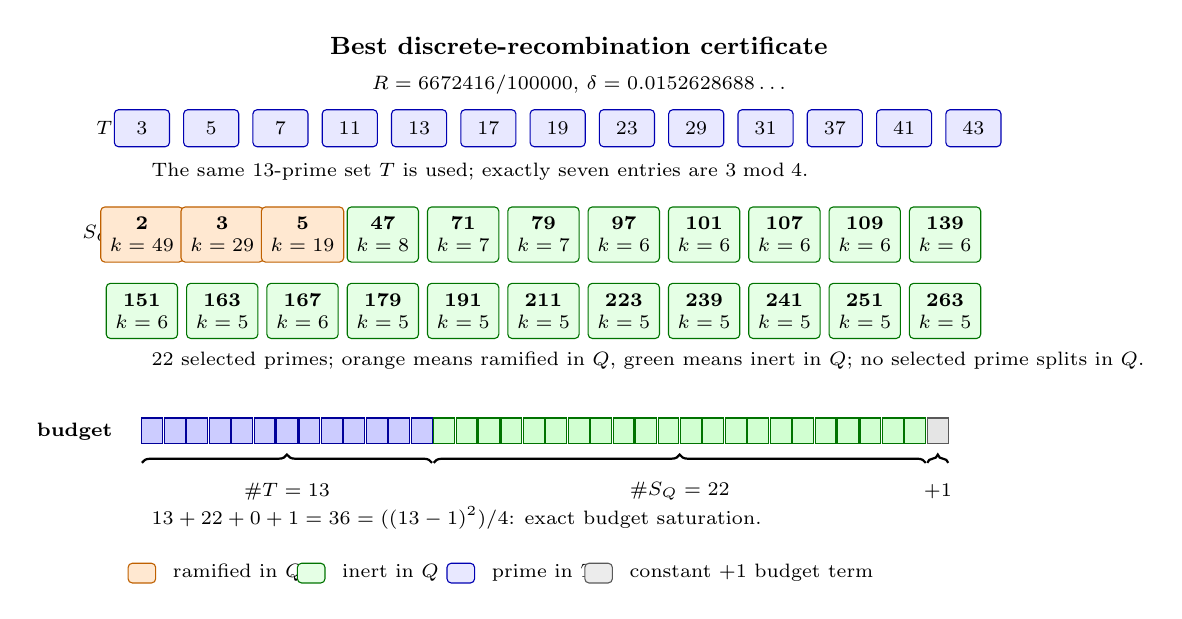
\begin{tikzpicture}[
  font=\scriptsize,
  tcell/.style={draw=blue!70!black, fill=blue!9, rounded corners=1.5pt, minimum width=0.70cm, minimum height=0.47cm, align=center},
  inertcell/.style={draw=green!45!black, fill=green!10, rounded corners=1.5pt, minimum width=0.90cm, minimum height=0.70cm, align=center},
  ramcell/.style={draw=orange!75!black, fill=orange!18, rounded corners=1.5pt, minimum width=0.90cm, minimum height=0.70cm, align=center},
  basecell/.style={draw=gray!70!black, fill=gray!15, rounded corners=1.5pt, minimum width=0.35cm, minimum height=0.25cm, align=center},
  note/.style={align=left, font=\scriptsize},
  lab/.style={font=\scriptsize\bfseries, anchor=east}
]
\node[font=\small\bfseries, align=center] at (5.55,1.05) {Best discrete-recombination certificate};
\node[note, align=center] at (5.55,0.55) {$R=6672416/100000$, $\delta=0.0152628688\ldots$};

\node[lab] at (-0.25,0) {$T$};
\foreach \p [count=\i from 0] in {3,5,7,11,13,17,19,23,29,31,37,41,43} {
  \node[tcell] at (\i*0.88,0) {\p};
}
\node[note, anchor=west] at (0,-0.55) {The same 13-prime set $T$ is used; exactly seven entries are $3\bmod 4$.};

\node[lab] at (-0.25,-1.35) {$S_Q$};
\foreach \p/\k/\sty [count=\i from 0] in {2/49/ramcell,3/29/ramcell,5/19/ramcell,47/8/inertcell,71/7/inertcell,79/7/inertcell,97/6/inertcell,101/6/inertcell,107/6/inertcell,109/6/inertcell,139/6/inertcell} {
  \node[\sty] at (\i*1.02,-1.35) {\textbf{\p}\\$k=\k$};
}
\foreach \p/\k/\sty [count=\i from 0] in {151/6/inertcell,163/5/inertcell,167/6/inertcell,179/5/inertcell,191/5/inertcell,211/5/inertcell,223/5/inertcell,239/5/inertcell,241/5/inertcell,251/5/inertcell,263/5/inertcell} {
  \node[\sty] at (\i*1.02,-2.32) {\textbf{\p}\\$k=\k$};
}
\node[note, anchor=west] at (0,-2.95) {22 selected primes; orange means ramified in $Q$, green means inert in $Q$; no selected prime splits in $Q$.};

\node[lab] at (-0.25,-3.85) {budget};
\foreach \i in {0,...,12} {\draw[draw=blue!60!black, fill=blue!20] ({0.285*\i},-4.00) rectangle ++(0.265,0.32);} 
\foreach \i in {13,...,34} {\draw[draw=green!45!black, fill=green!18] ({0.285*\i},-4.00) rectangle ++(0.265,0.32);} 
\draw[draw=gray!70!black, fill=gray!20] ({0.285*35},-4.00) rectangle ++(0.265,0.32);
\draw[decorate, decoration={brace, amplitude=3pt}, thick] (0,-4.25) -- ({0.285*13-0.02},-4.25) node[midway, yshift=-0.36cm] {$\#T=13$};
\draw[decorate, decoration={brace, amplitude=3pt}, thick] ({0.285*13},-4.25) -- ({0.285*35-0.02},-4.25) node[midway, yshift=-0.36cm] {$\#S_Q=22$};
\draw[decorate, decoration={brace, amplitude=3pt}, thick] ({0.285*35},-4.25) -- ({0.285*36-0.02},-4.25) node[midway, yshift=-0.36cm] {$+1$};
\node[note, anchor=west] at (0,-4.95) {$13+22+0+1=36=((13-1)^2)/4$: exact budget saturation.};

\node[ramcell, minimum width=0.35cm, minimum height=0.25cm] at (0,-5.65) {};
\node[anchor=west] at (0.27,-5.65) {ramified in $Q$};
\node[inertcell, minimum width=0.35cm, minimum height=0.25cm] at (2.15,-5.65) {};
\node[anchor=west] at (2.42,-5.65) {inert in $Q$};
\node[tcell, minimum width=0.35cm, minimum height=0.25cm] at (4.05,-5.65) {};
\node[anchor=west] at (4.32,-5.65) {prime in $T$};
\node[basecell] at (5.80,-5.65) {};
\node[anchor=west] at (6.07,-5.65) {constant $+1$ budget term};
\end{tikzpicture}}
\caption{Parameter-level visualization of the best certificate found by the Tailored Integer Evolution Strategy with discrete recombination.  The figure records the finite data that are checked by the verification script; it is not a coordinate realization of the corresponding asymptotic planar construction.}
\label{fig:recomb-candidate-dashboard}
\end{figure}

The arithmetic checks again pass.  Formula~\eqref{eq:delta-objective} gives
\[
\begin{aligned}
\text{numerator}   &=4.5232596663564752\ldots,\\
\text{denominator} &=296.35710825977047\ldots,\\
\delta             &=0.01526286881700719\ldots .
\end{aligned}
\]
This is a small improvement over the non-recombining Tailored Integer Evolution Strategy certificate, whose value was $0.01526166106841929\ldots$.

\begin{remark}[Algorithmic side experiments]
Discrete recombination was beneficial in the recorded run, but only marginally.  A self-adaptive mutation-rate variant was also tested; it did not produce a better certificate than the simpler Tailored Integer Evolution Strategy, apparently because the strategy parameter converged prematurely to a narrow local optimization regime.  For this reason, the self-adaptive variant is not used as the main reported optimization result.
\end{remark}

\begin{remark}[Status of the claim]
The verification attempts passed all checks implemented in the self-contained implementation: primality, parity of $T$, admissibility of the primes in $S_Q$, absence of split primes in $Q$, exact saturation of the Golod--Shafarevich budget, positivity of all $k(p)$, $R>1$, and the numerical inequalities for the stated clean exponents.  Thus the fixed-$T$ part of the bundle supports a sequence of certificate-level lower-bound improvements relative to Sawin's published $n^{1.014}$ statement: first the greedy certificate, then the Tailored Integer Evolution Strategy certificate, and finally the discrete-recombination variant.  The subsequent Cordella enlarged-$T$ subsection records a stronger verified addendum certificate on a different ramification scale.  However, the sharper displayed decimal values should still be treated with the usual caution until independently checked with interval arithmetic and reviewed by a human expert in the number-theoretic construction.
\end{remark}

\subsection*{Verified Cordella enlarged-$T$ example}

The canonical data communicated for Cordella's enlarged-$T$ example are now checked by the same verification pipeline as the four fixed-$T$ examples above.  The certificate uses the first 67 odd primes as the ramified set,
\[
T=\{3,5,7,\ldots,331,337\},\qquad \#T=67,
\]
so that 35 elements of $T$ are congruent to $3\bmod 4$.  The parity condition is therefore satisfied.  The scalar parameter is
\[
R=33066458/1000000=33.066458.
\]
The selected set $S_Q$ contains 1021 primes.  To keep the printed appendix compact, the non-unit multiplicities are listed by level; all remaining selected primes in $S_Q$ have multiplicity one.  The complete 1021-entry list is included in the ancillary certificate data file and in the generated verification JSON.


\begin{center}
\scriptsize
\begin{tabular}{r p{0.74\linewidth}}
\toprule
$k(p)$ & primes $p$ with this multiplicity\\
\midrule
22 & 2\\
14 & 3\\
9 & 5\\
7 & 7\\
6 & 11\\
5 & 13, 17\\
4 & 19, 23, 29, 31\\
3 & 37, 41, 43, 47, 53, 59, 61, 67, 71, 73, 79, 83, 89, 97\\
2 & 101, 103, 107, 109, 113, 127, 131, 137, 139, 149, 151, 157, 163, 167, 173, 179, 181, 191, 193, 197, 199, 211, 223, 227, 229, 233, 239, 241, 251, 257, 263, 269, 271, 277, 281, 283, 293, 307, 311, 313, 317, 331, 337, 347, 353, 359, 373, 379, 401, 431, 439, 443, 457, 467, 479, 491, 499, 509, 547, 557, 563, 571, 577, 587, 593, 607, 617, 619, 641, 643, 647, 653\\
1 & 924 remaining selected primes in $S_Q$, from 673 through 16529, as listed in the ancillary certificate file\\
\bottomrule
\end{tabular}
\end{center}

The exact integer product $D=\prod_{q\in T}q$ has 136 decimal digits; it is stored explicitly in the verification output.  The implemented arithmetic checks give
\[
\#\{p\in S_Q:p\text{ splits in }\mathbb Q(\sqrt D)\}=0,
\]
and the Golod--Shafarevich budget is exactly saturated:
\[
67+1021+0+1=1089=\frac{(67-1)^2}{4}.
\]
The numerical components returned by the verification pipeline are
\[
\begin{aligned}
\text{numerator}   &=138.0108764421359612998694861\ldots,\\
\text{denominator} &=4425.505735511937046245650675\ldots,\\
\delta             &=0.031185334443176590595661471677599365\ldots .
\end{aligned}
\]
All implemented checks pass: primality of $T$ and $S_Q$, oddness and parity of $T$, positivity of all multiplicities, $R>1$, absence of split primes in $S_Q$, the saturated budget inequality, and the admissibility-witness check.  This makes the Cordella enlarged-$T$ example the strongest verified certificate in the present appendix.  Under the same caveat as throughout the report--namely that Sawin's explicit criterion is being applied as cited--it supports the clean statement $u(n)>n^{1.0311}$ for arbitrarily large $n$.

\begin{proposition}[Verified enlarged-$T$ addendum certificate]
The canonical Cordella enlarged-$T$ certificate described above passes the verification pipeline and has exponent gain
\[
\delta=0.031185334443176590595661471677599365\ldots .
\]
In particular, it improves the fixed-$T$ certificates verified earlier in the appendix.
\end{proposition}

\newpage
\section*{Dedication}

\textit{Dedicated to the memory of G\"unter Rudolph}.

\section*{Acknowledgements}

The author thanks the researchers and engineers who created and openly released the 2026 counterexample material, and Noga Alon, Thomas F. Bloom, W. T. Gowers, Daniel Litt, Will Sawin, Arul Shankar, Jacob Tsimerman, Victor Wang, and Melanie Matchett Wood for the human-verified exposition.  The author is especially grateful to Will Sawin for the explicit quantitative lower bound and for making the associated parameter-selection problem visible.  The author also thanks Francesco Cordella for sharing the enlarged-$T$ communication on 4 June 2026 after publication of v1 and for permitting it to be recorded as an addendum.  Any remaining errors or overinterpretations are the author's responsibility.

\begin{thebibliography}{9}

\bibitem{Erdos1946}
P. Erd\H{o}s, ``On sets of distances of $n$ points,'' \emph{American Mathematical Monthly}, vol. 53, no. 5, pp. 248--250, 1946.

\bibitem{ST1983}
E. Szemer\'edi and W. T. Trotter, ``Extremal problems in discrete geometry,'' \emph{Combinatorica}, vol. 3, pp. 381--392, 1983.

\bibitem{SST1984}
J. Spencer, E. Szemer\'edi, and W. T. Trotter, ``Unit distances in the Euclidean plane,'' in \emph{Graph Theory and Combinatorics}, Academic Press, 1984, pp. 294--304.

\bibitem{OpenAI2026}
OpenAI, ``An OpenAI model has disproved a central conjecture in discrete geometry,'' May 20, 2026.  Available at \url{https://openai.com/index/model-disproves-discrete-geometry-conjecture/}.

\bibitem{AlonEtAl2026}
N. Alon, T. F. Bloom, W. T. Gowers, D. Litt, W. Sawin, A. Shankar, J. Tsimerman, V. Wang, and M. Matchett Wood, ``Remarks on the disproof of the unit distance conjecture,'' arXiv:2605.20695, 2026.  Available at \url{https://arxiv.org/abs/2605.20695}.

\bibitem{Sawin2026}
W. Sawin, ``An explicit lower bound for the unit distance problem,'' arXiv:2605.20579, 2026.  Available at \url{https://arxiv.org/abs/2605.20579}.


\bibitem{Cordella2026}
F. Cordella, ``Enlarging the ramified prime set in Sawin-style unit-distance certificates,'' personal communication and draft/report shared with M. T. M. Emmerich on 4 June 2026, after publication of v1.

\bibitem{Rudolph1994}
G. Rudolph, ``An evolutionary algorithm for integer programming,'' in Y. Davidor, H.-P. Schwefel, and R. M\"anner, Eds., \emph{Parallel Problem Solving from Nature -- PPSN III}, Lecture Notes in Computer Science, vol. 866, Berlin, Heidelberg: Springer, 1994, pp. 139--148. doi: \href{https://doi.org/10.1007/3-540-58484-6_258}{10.1007/3-540-58484-6\_258}.

\bibitem{FejesToth1942}
L. Fejes T\'oth, Ueber die dichteste Kugellagerung, \emph{Mathematische Zeitschrift} 48 (1942), 676--684. doi:10.1007/BF01180035.

\end{thebibliography}

\end{document}
